% Paper "Shalika Germs on GSp(4)"
% Author: Thomas C. Hales
% Hales, Thomas C. "Shalika germs on GSp (4)." Ast�risque 171-72 (1989): 195-256.
%

\documentclass{amsart}

\usepackage{amssymb}
\usepackage{amsthm}
\usepackage{enumitem}
\usepackage{amsrefs}
\usepackage{tikz} 
\usetikzlibrary{chains,shapes,arrows,shadings,trees,matrix,%
  positioning,intersections,decorations,%
  decorations.markings,decorations.pathmorphing,backgrounds,%
  fit,calc,fadings,decorations.pathreplacing}

\begin{document}

\newcommand{\dsize}{\displaystyle} 
\newcommand{\wasacaption}[1]{#1}

\font\smc=cmcsc10
\def\proclaim#1{\medbreak\medskip\noindent 
  {\smc#1.\enspace}\sl} 
\def\endproclaim{\par\rm 
  \ifdim\lastskip<\medskipamount\removelastskip 
  \penalty55\medskip\fi} 


\def\smalldot#1{\draw[fill=black] (#1) node [inner sep=1.3pt,shape=circle,fill=black] {}}
\def\graydot#1{\draw[fill=gray] (#1) node [inner sep=1.3pt,shape=circle,fill=gray] {}}
\def\whitedot#1{\draw[fill=gray] (#1) node [inner sep=1.3pt,shape=circle,fill=white,draw=black] {}}


\title{Shalika Germs on $GSp(4)$}
\author{Thomas C. Hales}
\address{Harvard University}
\thanks{Ast\'erisque 171-72 (1989): 195--256.}
\thanks{This preprint version differs slightly from the published version.}


%\input vanilla.sty
%\scaletype{\magstep1}
%\overfullrule=0pt
%\pagewidth{6.9 truein}
%\pageheight{9.875 truein}
%\hcorrection{-.2in}
%\vcorrection{-.5in}
%\nopagenumbers
\baselineskip = 18pt
%\hrule height0pt width6true in
%\vskip 1.3true in

%\heading
%\title 
%Shalika Germs on $GSp(4)$
%\endtitle
%\endheading

%\heading
%Thomas C. Hales
%\endheading

%\vskip .8in

\begin{abstract}
This paper calculates all of the Shalika germs of the group  $GSp(4)$  and its
inner forms over a local $p$-adic field of characteristic zero.  As a 
consequence we conclude that the conjectures of  Langlands and Shelstad [LS2],
relating linear combinations of germs on a reductive group $G$ to germs on the
endoscopic groups of  $G$, are valid for  $G = GSp(4)$  or one of its inner
forms.  A further consequence is that all stable germs associated to the non-special
unipotent class are identically zero.  More generally, when  $G = Sp(4)$  or one
of its inner forms we show that the germs associated to the regular and subregular
unipotent classes satisfy the conjectures of Langlands and Shelstad.
\end{abstract}

\maketitle

\S 1 \quad A Review of Igusa Theory

\S 2 \quad Background on Shalika Germs

\S 3 \quad A variety    which computes Shalika Germs

\S 4 \quad The symplectic group

\S 5 \quad The transfer of subregular germs of $Sp(4)$

\S 6 \quad The transfer of 2-regular germs of  $GSp(4)$

\S 7 \quad Spurious divisors and some technical details.
%\vglue 0in plus 3in
%\hrule height 0pt width 6in depth 0pt
%\pagebreak
\vskip .4in

\section{A Review of Igusa Theory}


The approach to calculating Shalika germs used here was introduced by R.P. Langlands
in [L].  This paper fixes the group\ $GSp(4)$\   and studies all of its germs.  This should
be contrasted with [H] which studies a particular germ, that associated to the 
subregular unipotent classes, for all reductive groups.  The essential ingredient
is a theorem of Igusa on asymptotic expansions.  For the sake of completeness we
restate the theorem.
\vskip .2in

\noindent 1.~~  Let $X$  be a smooth variety over a curve $\Gamma~~(X~
^{\underrightarrow{\varphi}}~\Gamma)$  with  $X,\Gamma$ and  $\varphi$  defined 
over a local $p$-adic field $F$ of characteristic zero.
\vskip .2in

\noindent 2.~~ Suppose that there is a point  $x_0$  on  $\Gamma(F)$  such that
$X$  is smooth outside\ $\varphi^{-1}(x_0)$\  and  $\varphi^{-1}(x_0)$\ is a
divisor with normal crossings with the property that any irreducible component
of  $\varphi^{-1}(x_0)$\ with an $F$-rational point is defined over  $F$.  Let
$\mathcal E$ be the set of irreducible components of  $\varphi^{-1}(x_0)$\ defined
over  $F$.  Let\ $a(E)$\ for\ $E\in {\mathcal E}$\ be the multiplicity of $E$  in\
$\varphi^{-1}(x_0)$.
\vskip .2in

\noindent 3.~~ Let  $\omega$  be a form of maximal degree on  $X$  which is 
defined over the algebraic closure  $\overline{F}$  of $F$  which is nonvanishing
and regular outside\ $\varphi^{-1}(x_0)$.\ Write the divisor of $\omega$ as
$D + \dsize\sum_{E\in{\mathcal E}} (b(E)-1)E$\ with\ $b(E)\in{\bold Z}$.  We may
ignore the term $D$ having no $F$-rational points.
\vskip .2in

\noindent 4.  Suppose that there is a torus $T$ over $F$  which is split by a
Galois extension  $E/F$  and rational functions\ $t_\sigma \in T(K_E)$\  for
$\sigma\in Gal(E/F)$\ and  $K_E$  the field of rational functions on\
$X \times_{Spec(F)} Spec(E)$.\ Suppose that $t_\sigma$\ defines a cohomology
class\  $[t_\sigma]_p$\  of  $H^1(Gal(E/F), T(E))$\  for $F$-rational points
$p$  in a Zariski open set of  $X$  and that\ $p\mapsto [t_\sigma]_p$\ extends to
a locally constant function on the $F$-rational points of  $X\setminus \varphi^{-1}(x_0)$.
For any character $\kappa$ of\ $H^1(Gal(E/F), T(E))$\ and divisor  $D\in{\mathcal E}$\ we
define a character  $\kappa_D$  of  $F^\times$ ~~ $(\kappa_D:  F^\times \to {\bold C}^\times)$\ as follows.
Pick local $p$-adic coordinates  $\mu_1,\ldots ,\mu_n$\  over  $F$  at
$p_0\in D(F)$\ such that\ $\mu_1 = 0$\ defines $D$  locally.  Choose, if possible,
$\kappa_D$  so that  $\kappa(t_\sigma)/\kappa_D(\mu_1)$\  extends to a function
constant in a neighborhood of  $p_0$.  If  $p_0$\ lies in no other divisor of
${\mathcal E}$\ then such a character exists and is independent of  $p_0\ \in D(F)$\
and the choice of local coordinates.
\vskip .2in

\noindent 5.~~ If $\theta$  is a character of finite order of  $F^\times$ and
$\beta \in {\bold Q}$  let  ${\mathcal E}(\theta,\beta)$\ be the set of divisors in ${\mathcal E}$
such that  $\theta^{a(E)} = \kappa_E$  and  $b(E)/a(E) = \beta$.  Let  $e(\theta,\beta)$\
be the maximum number of divisors of  ${\mathcal E}(\theta,\beta)$\ with non-empty
intersection.
\vskip .2in

\noindent 6.~~ Let  $f$  be a locally constant function on  $X$  whose support is
proper over  $\Gamma$.
\vskip .2in

\noindent 7.~~ Normalize the valuation on $F$  by the additive Haar measure  $dx$  so 
that  $d(ax) = |a|dx$  and set  $m(\lambda) = - log_q|\lambda|$  where  $q$
is the order of the residue     field of  $F$.  Extend, whenever necessary,
$|\cdot |$\ to extensions  $E$ of $F$.  Normalize the Haar measure  $dx$  so that
$\int_{|x|\le 1} dx = 1$.  Finally let $\lambda$  be a local
$F$-parameter on $\Gamma$  such that\ $\lambda = 0$\ defines the point
$x_0$.
\vskip .2in
		      
%\pagebreak
\proclaim{Proposition\ \ 1.1}  In the above situation, for  $|\lambda |$ sufficiently
small there is an expansion
$$
F(\lambda)\ {\mathrel{\mathop=^{def}}}\ \int_{\varphi^{-1}(\lambda)} \kappa(t_\sigma)f 
{\frac{|\omega|}{|\varphi^*(d\lambda)|}} = \sum \theta (\lambda )|\lambda |^{\beta -1}
\sum^{e(\theta,\beta)}_{r=1} m(\lambda)^{r-1} F_r(\theta,\beta) .
$$
The first sum runs over  $(\theta,\beta)$\ with  ${\mathcal E}(\theta,\beta)$\
nonempty.  $F_r(\theta,\beta)$\ is independent of $\lambda$  but depends on
$r,\theta,\beta,f,\kappa$.
\endproclaim



\begin{proof}  See [L] for a proof and details.  The only difference in our
presentation is that [L] incorporates  $\kappa(t_\sigma)$\ directly into the definition
of  $f$  which is not assumed to be locally constant.  
\end{proof}

We also need the explicit
formula for  $F_r(\theta ,\beta)$\ when\ $e(\theta ,\beta ) = 1,2$.  Begin
with  $e(\theta ,\beta ) = 1$.  By construction  $\kappa(t_\sigma)/\theta(\lambda)$
extends generically to  $E \in {\mathcal E}$.  Let  $m_{\theta,E}$  be its restriction to
$E$.  By construction $\omega/(\lambda^{\beta -1}d\lambda)$
extends generically to  $E$.  Let  $\omega_E$  be its restriction.  Since  $\beta$
is rational  $\omega_E$  is defined up to a root of unity.  Then we have
\begin{equation}\tag{1.2}
F_1(\theta,\beta) = \sum_{E\in{\mathcal E}(\theta,\beta)} PV \int_E m_{\theta,E} f |\omega_E|.
%\tag 1.2
\end{equation}


\noindent A principal value integral is required since  $\omega_E$  may have poles
and  $m_{\theta,E}$  might not be locally constant.  Now let  $e(\theta,\beta) = 2$.
We proceed as before but along the intersection of two divisors  $E,E'$  in
${\mathcal E}(\theta,\beta)$\ the forms  $\omega_E$  and  $\omega_{E'}$\  have simple
poles, and the principal value integrals  $PV \int_E m_{\theta,E} f |\omega_E|$  
diverge.  The difficulty stems from the fact that the form  $dx/x$  is scale
invariant.  The problem is overcome by truncating the integral on  $E$  and  $E'$
near the pole and adding a principal value integral on $E\cap E'$.  We continue
to write  $F_1(\theta,\beta)$  as a sum of integrals over divisors but when
$e(\theta,\beta) = 2$  the integrals must be regularized in this manner.
\vskip .2in

\proclaim{Lemma\ \ 1.3}  Suppose that  $\lambda = \alpha\mu_1^{a_1} \ldots \mu_n^{a_n}$
in local $p$-adic $F$-coordinates on a patch $U$ containing\ $p\in D(F), D = E_1 \cap E_2$,
that  $\mu_i = 0$\ defines $E_i, ~ i = 1,2$, $a_1 = a_2 = 1$, $b_1 = b_2$, and\ 
$E_i \in {\mathcal E}(\theta,\beta)$\, $i = 1,2$,\  for some  $(\theta,\beta)$.  Set
$$
\omega_D =  Residue_D \omega_{E_1} = \left. {\frac{\omega_{E_1}}{{\frac{d\mu_2}{\mu_2}}}}
\right|_D = Residue_D \omega_{E_2},~~{\text and}~~m_{\theta,D} = \left. m_{\theta,E_1}\right|_D =
\left. m_{\theta,E_2}\right|_D.
$$
\noindent Suppose that  $U$  is chosen small enough that  $m_{\theta,D}f$\ is
independent of  $\mu_1$  and  $\mu_2$  on\ $U \cap D_1$,\ and\ $|\alpha|$\ is
constant on  $U$.\ Suppose that the integrals on  $E_i$  are truncated by  $|\mu_i| \ge
q^{-m_i}$,\ $i = 1,2$,\  then the contribution to the term $F_1(\theta,\beta)$  from the pole
$D$  is given locally by
$$
(1 - {\frac{1}{q}}) \int_U  m_{\theta,D} (1-M) f |\omega_D| .
$$

%\pagebreak
where  $M = m(\alpha) + a_1m_1 + a_2m_2 + \sum_{i>2} 
a_im(\mu_i)$.
\endproclaim

\begin{proof}  This is a special case of the general formula found in [L].
\end{proof}
\vskip .4in

%2
\section{Background on Shalika Germs}


Let $G$  be a reductive group over a $p$-adic local field $F$ of characteristic
zero, and let  $T$ be a Cartan subgroup over $F$.  For every unipotent orbit
$O$  in  $G(F)$  let  $\mu_0$  denote an invariant measure on $O$.  Let  $dg$
be an invariant measure on\ $T(F)\setminus G(F)$.\  Shalika [Sh] has shown that
there exist functions\ $\Gamma_0(\gamma)$\  called germs defined on the regular
elements of  $T(F)$  for all unipotent classes $O$  in  $G(F)$  such that for
every  $f\in C^\infty_c(G)$\ , the space of locally constant functions of
compact support on  $G(F)$,  there is a neighborhood  $V_f$  of the identity
element in  $T(F)$  in which the expansion
$$
\int_{T(F)\setminus G(F)} f(x^{-1}\gamma x)dg = \sum_0 \mu_0(f)\Gamma_0(x)~~
{\text{holds~for}}~~\gamma~~{\text{regular~in}}~~V_f.
$$

\noindent If  $g\in (T\setminus G)(F)$,  then $\sigma(g)g^{-1}$  for
$\sigma\in Gal(\overline{F}/F)$  defines a cocycle of  $H^1(Gal(\overline{F}/F),T)$.
Now let  $dg$  denote an invariant measure associated to an invariant form on
$T\setminus G$.   Similarly normalize measures $\mu_0$  on unipotent
classes belonging to the same stable conjugacy class by fixing an invariant form
on the stable conjugacy class.  For  $h\in G(\overline{F})$  such that  $\sigma(h)h^{-1}$
gives a cocycle of  $Gal(\overline{F}/F)$  in  $Z$  the center of  $G$,  define
$f_h$  by  $f_h(x) = f(h^{-1}xh)$.  Let  $\kappa$  be a character on 
$H^1(Gal(\overline{F}/F), T)$. 

We form a $\kappa$-orbital integral and take its germ expansion:
$$
\Phi^{T,\kappa}(\gamma,f)\ {\mathrel{\mathop =^{def}}}\  \int_{(T\setminus G)(F)}
\kappa(\sigma(g)g^{-1})f(g^{-1}\gamma g)dg  = \sum_0 \mu_0(f)\Gamma_0^{T,\kappa}(\gamma)
\qquad \gamma~~ {\text{in}}~~ V_f .
$$

\noindent  Comparing the $\kappa$-orbital integrals of  $f$  and  $f_h$  it follows
easily that		     
\begin{equation}\tag{2.1}
\Gamma^{T,\kappa}_{0^h} = \Gamma_0^{T,\kappa} \kappa(\sigma(h)h^{-1}) . %\tag 2.1
\end{equation}

The character  $\kappa$  restricted to  $H^1(Gal(\overline{F}/F),Z)$\ depends only on
the endoscopic group  $H$  defined by  $(T,\kappa)$  and not directly on  $T$~~(see
for instance [H]).  For
background on endoscopic groups see [L2].  We may therefore write 
for an {\it adjoint} conjugacy class  $O$ (that is, the inverse image of an
F-orbit in the adjoint group)
\begin{equation}\tag{2.2}
\mu^H_{O}\ {\mathrel{\mathop=^{def}}}\ 
\sum  \mu_{0'} \kappa(\sigma (h) h^{-1})     %\tag 2.2
\end{equation}
\noindent The sum runs over all $F$-classes  $O'$  in the adjoint class, and  $h$  is
determined by  $O'\ = O_1^h$\ for a fixed $F$-class $O_1$ in $O$.  Using this fixed choice
$O_1 \subseteq O$\ write  $\Gamma_{O}^{T,\kappa}$  for  $\Gamma_{O_1}^{T,\kappa}$.  
Then the germ expansion becomes
\begin{equation}\tag{2.3}
\Phi^{T,\kappa} (\gamma,f) = \sum_{O~{\text adjoint}} \mu^H_{O}(f)
\Gamma_{O}^{T,\kappa} (\gamma).  %\tag 2.3
\end{equation}

\noindent  All ordinary orbital integrals may be recovered as linear combinations of
$\kappa$-orbital integrals.  One advantage of considering $\kappa$-orbital interals instead
of ordinary orbital   integrals is that one is able to group  $F$-classes belonging
to the same adjoint class together in this way.  In all that follows a germ is
associated to an {\it adjoint} unipotent conjugacy class using the measures
$\mu^H_0$.

We will make use of the following results from Harish-Chandra and Rogawski.  
Say that an orbit $O$  is $r$-regular if  $r = (\dim~C_G(u)-rank~G)/2$\  for\
$u\in O$.  If\ $r = 0,1$  the classes are also called regular and
subregular respectively.  Let  $Z^0_G$  be the connected center of  $G$.   For
details on normalizations of measures and proofs we refer to [H-Ch] and [R].

\proclaim{Proposition\ \ 2.4}\  
\begin{enumerate}[label=(\arabic*)]
\item If  $z\in Z^0_G(F)$  and  $\gamma\in T(F)$
lie sufficiently close to the identity then\ $\Gamma^{T,\kappa}_{O}(z\gamma)
= \Gamma^{T,\kappa}_{O}(\gamma)$.

\item If  $X\in Lie~G(F)$\  is regular and  $\exp(X)$\ is sufficiently
close to the identity then
$$
\Gamma^{T,\kappa}_{O} (\exp(t^2X)) = |t|^{2(r-r_0)} \Gamma_{O}^{T,\kappa}(\exp(X))
$$
\noindent for  $t\in F^\times$  sufficiently small for every  $r$-regular class
$O$,  $r_0 = (\dim~ G-rank~ G)/2$.

\item  Let $M$  be the connected centralizer of a semisimple element
$\gamma_0$  in $T$.  Then for every   $f\in C^\infty_c(G)$\ there exists\
$f^M \in C_c^\infty(M)$\ such that
$$
\Phi^T_G(\gamma,f) = \Phi^T_M(\gamma,f^M)
$$
\noindent for regular elements $\gamma$ in a sufficiently small neighborhood $V_f$
of $\gamma_0$ in  $T(F)$.
\end{enumerate}
\endproclaim
\vskip .2in

(2.5)~~Statement (2.4.1) tells us that the centers are mostly irrelevant to the
study of germs.  By passing to the derived group and then to the simply connected
cover we may assume that  $G$  is simply connected or semi-simple.  Notice that
the function  $\kappa(\sigma(g)g^{-1})$  on  $(T\setminus G)(F)$\ always pulls back to
the simply connected cover  $G_{sc}$\ of the derived group and that\ $T_{sc}\setminus G_{sc}
\to T\setminus G$\  is an isomorphism over  $F$.  Also $(T_{sc},\kappa_{sc})$ 
defines an endoscopic group $H'$ of $G_{sc}$ which differs from the endoscopic 
group $H$ of $G$ defined by $(T,\kappa)$ only by a central factor.
The simply connected semi-simple
group is more difficult to deal with than say the adjoint group because there are
more endoscopic groups associated to the simply connected groups.

(2.6)~~By combining (2.4.3) with (2.4.1) writing  $T = T_1Z_M$\  where
$T_1 \subseteq M_{der}$  for sufficiently small  $\gamma_1\in T_1(F)$,  and
sufficiently small
$z_1,z_0 \in Z^0_M(F)$\ we have
$$
\Phi^T_G(\gamma_1 z_1z_0,f) = \Phi^T_G(\gamma_1 z_0,f)
$$

\noindent provided\ $C_G(z_0)^0 = M$.  Thus we may consider the germs of
the expansion of\ $\Phi^T_G(\gamma,f)$\ near $z_0$  as functions on  $T_1$
alone instead of $T$.

(2.7)~~Langlands and Shelstad [LS2] have defined transfer factors $\Delta_G^{T,\kappa}(\gamma)$
and have conjectured that for every\ $f\ \in C_c^\infty(G)$\ there exists a
function  $f^H\in C_c^\infty(H)$  on the endoscopic group $H$ associated to  $(T,\kappa)$ such that
identifying Cartan subgroups in $H$ and $G$ we have
\begin{equation}\tag{2.8}
\Delta_G^{T,\kappa} \Phi^{T,\kappa}(\gamma,f)\ {\mathrel{\mathop=^?}}\ 
\Delta_H^{T,st}\Phi^{T,st}(\gamma,f^H) 
%\tag 2.8
\end{equation}

\noindent for all $(T,\kappa)$  associated to  $H$.  The integral on the right is a
{\it stable} orbital integral on  $H$  (that is, the character $\kappa$ is trivial).
We define  $\Delta^{T,\kappa}_G$  for  $\gamma$  regular and sufficiently close
to $1$  for  $G$  quasi-split by the condition
\begin{equation}
\Delta_G^{T,\kappa} \Phi_G^{T,\kappa}(\gamma ,f) = \mu_0^H(f)  \tag{2.9}
\end{equation}
for $0$  the regular adjoint unipotent class and  $f$  supported on regular elements
of  $G$.  The factor  $\Delta_H^{T,st}$\ is defined similarly.  Implicit in our
definition of transfer factors is a choice of measure  $\mu_0^H$.\ In [LS2] the
factors\ $\Delta_G^{T,\kappa}$\ and\ $\Delta_H^{T,st}$\  are combined into a
canonically defined single factor but they show the definition by (2.9) is
equivalent to theirs (up to a scalar).  For the reduction of this problem (2.8) to the problem of matching germ expansions of
$\Delta^{T,\kappa} \Phi^{T,\kappa}$\ and\ $\Delta_H^{T,st}\Phi^{T,st}$\  
near the identity element see [LS3].
\vskip .2in


Proposition (2.4) remains true with minor modifications when the transfer
factor is included.  From this point on we shift notation to let\ $\Gamma_0^{T,\kappa}$\
be the germ of\ $\Delta^{T,\kappa}\Phi^{T,\kappa}$.  By (2.9) we conclude that
(2.4.1) holds for $G$ quasi-split.  More generally, [LS2] shows that there is a
character $\theta$ of  $Z^0_G$  such that\  $\Delta(z\gamma) = \theta(z)\Delta(\gamma)$.\
By the explicit
description of the transfer factor in [LS2] (2.4.2) holds with  $r_0 = 0$.\ A
version of  (2.4.3) with transfer factors is proved in (2.11).

Statement (2.4.1)  gives a necessary condition
for the transfer of germs to an endoscopic group.  Identifying the connected
center  $Z^0_H$  of  $H$  with a subgroup\ $T\subseteq G$\ it says that the
germs of $\kappa$-orbital integrals on  $G$  associated to  $H$  should be invariant
by  $Z^0_H$.

The rest of this section shows, roughly speaking, that to prove  (2.6)
for a fixed  $(T,\kappa)$\ when
$H$  is a product  $H = H_1\times H_2$  it is often enough to prove that the
germs of\ $\Delta^{T,\kappa} \Phi^{T,\kappa}(\gamma,f)$\  have a decomposition of the
form\  $\Gamma_O^{T,\kappa} = \sum a_ib_i$\ where  $a_i$  are functions on
$T\cap (H_1\times \{ 1\})$  and  $b_i$  are functions on  $T\cap (\{ 1\} \times H_2)$.  Since the germs on a product of
groups equal the products of germs on the individual groups it is clear that such
a decomposition is a necessary condition for  (2.8)   to hold.  This section
does {\it not} show that the choice of  $f^H$  can be made independently of
$(T,\kappa)$.  This will be shown later in the special case
$G = GSp(4)$.

For any reductive group  $G$  let  $G_{qs}$  denote a quasi-split inner form of
$G$.  It is unique up to an isomorphism over $F$.  There is an injection of
stable conjugacy classes of Cartan subgroups in $G$ to stable conjugacy classes
of Cartan subgroups in  $G_{qs}$.  If  $T$  is a Cartan subgroup over $F$ in $G$, 
write  $T_{qs}$  for an image in  $G_{qs}$  and for  $\gamma\in T$  write
$\gamma_{qs}$  for the corresponding element in  $G_{qs}$.  $T$ and  $T_{qs}$
are then isomorphic over  $F$  and this isomorphism may be used to identify
characters on  $H^1(Gal(\overline{F}/F), T)$  and  $H^1(Gal(\overline{F}/F),T_{qs})$.

If  $S$  is a torus over  $F$  in  $G$  let  $C(S)$  denote its centralizer in 
$G$.

\proclaim{Definition\ \ 2.10} The $\kappa$-orbital  integrals on $G$  are said to have
{\it quasi-split~reduction}~ $(QSR)$ if for every triple $(S,T,\kappa)$, $1\ne S\subseteq T$,
$S$  torus over  $F$, $T$ Cartan subgroup over $F$, $\kappa$ character on
$H^1(Gal(\overline{F}/F),T)$\ and for every function\ $f\in C^\infty_c(C(S))$\
there exists a function\ $f_{qs} \in C^\infty_c(C(S)_{qs})$\ such that
$$
\Phi^{(T,\kappa)}_{C(S)}(\gamma,f) = \Phi^{(T_{qs},\kappa)}_{C(S)_{qs}}(\gamma_{qs},
f_{qs})
$$
\noindent for every  $\gamma\in T'(F)$  (the regular elements of $T$).  We note
that this condition is independent of the choice of  $T_{qs}$.
\vskip .2in

\proclaim{Proposition\ \ 2.11}  Suppose that  $G$  is quasi-split and the $\kappa$-orbital integrals of  $G$  have
quasi-split reduction.  Let  $(S,T,\kappa)$  be a triple as in the definition of
$QSR$.  Let  $f\in C^\infty_c(G)$\ and let  $s\in S(F)$  be an element sufficiently
close to the identity such that
$C_G(s) = C(S)$.  Then there exists a neighborhood $V$ (depending on $f$) of $s$ in
$T(F)$  and a function $f_{qs}$  in  $C^\infty_c(C(S)_{qs})$\ (depending on  $s$)
such that
$$
\Delta_G^{T,\kappa} \Phi^{(T,\kappa)}_G (\gamma,f) = \Delta^{T_{qs},\kappa}_{C(s)_{qs}}
\Phi^{(T_{qs},\kappa)}_{C(S)_{qs}} (\gamma_{qs},f_{qs})
\qquad {\text for}\quad \gamma\in V\cap T'(F).
$$
\endproclaim

\begin{proof}  This is no more than (2.4.3)  combined with the 
definition of  $QSR$.  A few details will make this clear.
\end{proof}

Set  $M = C(S)$.        The map  $i:  T \hookrightarrow M$  gives
$i_*:  H^1(Gal(\overline{F}/F),T) \to H^1(Gal(\overline{F}/F),M)$.  If
$Tg\in (T\setminus G)(F)$  then the cocycle  $i_*(\sigma(g)g^{-1}), \sigma\in
Gal(\overline{F}/F)$  belonqs to  $H^1(Gal(\overline{F}/F),M)$.  Let  
$g_1,\ldots ,g_r \in G(\overline{F}), Tg_1,\ldots ,Tg_r \in (T\setminus G)(F)$\
be such that $i_*(\sigma(g_i)g_i^{-1}), i = 1,\ldots ,r$\ are representatives of 
the classes in  $H^1(Gal(\overline{F}/F),M)$\ so obtained.  Then  $M^{g_i}$  is
an inner form of  $M$.  Set  $T_i = T^{g_i}, M_i = M^{g_i}, \gamma_i =
\gamma^{g_i}$.
It is easy to check that  $(T\setminus G)(F)$  is a disjoint union of
$X_i = g_i((T_i\setminus M_i)(F))G(F)$, $i = 1,\ldots ,r$.  The $\kappa$-orbital
integral on  $G$  is an integral over  $(T\setminus G)(F)$  which breaks up
as a sum of integrals over the  $X_i$.  First we prove a version of
the proposition for each  $X_i$, i.e., that there exists $(f_i)_{qs} \in
C^\infty_c(M_{qs})$  such that
$$
\int_{(g_i^{-1}X_i)} \kappa_i(\sigma gg^{-1})f(g^{-1}\gamma_ig)dg = 
\Phi^{T_{qs},\kappa}_{M_{qs}} (\gamma_i, (f_i)_{qs})
$$

\noindent where  $\kappa_i$  is the character on  $H^1(Gal(\overline{F}/F),T_i)$\
obtained by identifying  $T$ and $T_i$  by the isomorphism $\gamma \mapsto \gamma_i$.

Let  $\epsilon^i_1,\ldots ,\epsilon^i_t$  be the elements of the image of
$(T_i\setminus M_i)(F)$\ in $H^1(Gal(\overline{F}/F),T_i)$ and let  $m^i_1,\ldots ,
m^i_t$  be representatives in$(T_i\setminus M_i)(F)$.  Then dropping super and
subscript  $i$'s on  $m^i_j\ \epsilon^i_j,  T_i$  we have, using the definition
of  $X_i$

\begin{align*}
\int_{g_i^{-1}X_i} & = \sum_j \kappa_i(\epsilon_j) 
\int_{T^{m_j}(F)\setminus G(F)} f(g^{-1}\gamma_i^{m_j}g)dg\\
&= \sum_j \kappa_i(\epsilon_j) \int_{T^{m_j}(F)\setminus M_i(F)} 
f_i(m^{-1} \gamma_i^{m_j}m)dm\qquad (\text{by~2.4.3})\\
&= \Phi^{T,\kappa}_{M_i} (\gamma_i,f_i)\\
&= \Phi^{T_{qs},\kappa}_{M_{qs}} (\gamma_{qs},(f_i)_{qs})\qquad {\text{by~the~
definition~of}}~~QSR  ~~ .
\end{align*}

\noindent Thus	 combining the  $X_i$ and  $(f_i)_{qs}$
$$
\Delta_G^{T,\kappa}\Phi_G^{T,\kappa}(\gamma,f) = \delta\ \Delta^{T_{qs},\kappa}_{M_{qs}}
\Phi^{T_{qs},\kappa}_{M_{qs}}(\gamma_{qs},f_{qs}') = \Delta^{T_{qs},\kappa}_{M_{qs}}
\Phi^{T_{qs},\kappa}_{M_{qs}}(\gamma_{qs}, \delta f_{qs}'),  \delta =
\Delta_G^{T,\kappa}/\Delta^{T_{qs},\kappa}_{M_{qs}} .  
$$

\noindent Fix $s$ small enough so that (2.9) holds, then this equation becomes
$\mu_0^H(f) = \delta \mu_{O'}^{H'}(f_{qs}')$\  where  $O'$  is the regular
unipotent class of  $M_{qs}$  and  $(T_{qs},\kappa)$\ defines the endoscopic
group  $H'$.  Thus  $\delta$  and hence  $f_{qs} = \delta f_{qs}'$\ depends on
$\gamma \in T(F),\ \gamma_{qs} \in T_{qs}(F)$\  only through  $s\in S(F)$\ in a
sufficiently small neighborhood of the identity and sufficiently near $s$.  The
proposition follows.
\vskip .2in

As above let  $G$  be a reductive group over a $p$-adic field $F$ of characteristic
zero, and let  $H$  be an endoscopic group of $G$.  Suppose that up to a finite 
center  $H$  is a product  $H_1 \times H_2$  over  $F$.  Then we associate to
$G$  and  $H$  an intermediate group  $M$  as follows.

Select a Cartan subgroup  $T$  over  $F$  in  $H$.  Corresponding to  $H_1\times H_2$ we
write  $T = T_1T_2$  with  $T_1\cap T_2$  finite.  Identify $T = T_1T_2$  with
a Cartan subgroup in  $G$.  It is determined up to stable conjugacy.  Let
$M = (C_G(T_1)\times C_G(T_2))/\{ (x,x^{-1}): x\in T\}$.  For example, if
$G = Sp(2n),\ H = Sp(2i)\times SO(2(n-i)),$\ then\ $M = Sp(2i)\times Sp(2(n-i))$.
\vskip .2in

\proclaim{Lemma\ \ 2.12}  $M_{qs}$  is independent of the choice of  $T\subseteq H$.
\endproclaim

\begin{proof}  It is enough to check that  $T$  and  $T' = T_1T'_2$  give the same
$M_{qs}$.  Select  $g\in Q(\overline{F})$\ such that\ $T_2^g = T'_2$\quad
where  $Q =\ C_G(T_1).$\ $C_{C_G(T_2)}(T_1T_2) =
C_G(T_1T_2) = T_1T_2$\  so  $T_1T_2$  is a Cartan subgroup of  $C_G(T_2)$.
It follows  that there is a Cartan subgroup $T_{der}$ 
of $C_G(T_2)_{der}$\  contained in  $T_1$.

If  $m\in C_G(T_2)_{der}~~\sigma\in Gal(\overline{F}/F)$\ then 
$\sigma(m)^{\sigma(g)g^{-1}g} = \sigma(m^g)$,\ $\sigma(g)g^{-1} = w_\sigma \in
N_Q(T_2)$.\  By the definition of  $Q$,  $t^{w_\sigma} = t$\  for\ 
$t\in T_{der}(\overline{F})\ (\subseteq T_1( \overline{F}))$.  
Since  $T_{der}$  is a Cartan subgroup, $w_\sigma \in T_{der}(\overline{F})$ so that
$C_G(T_2)_{der}$  and  $C_G(T'_2)_{der}$  are inner forms.  Using
$TC_G(T_2)_{der} = C_G(T_2),\ \quad TC_G(T'_2)_{der} = C_G(T'_2)$\  the result
follows easily.
\end{proof}
\vskip .2in

The following simple lemma is the key to what follows.

\proclaim{Lemma\ \ 2.13}  Let  $k$  be any field.  Let  $X,Y$  be sets endowed with
decreasing filtrations  $X = X_0 \supseteq X_1 \supseteq \ldots , 
Y = Y_0 \supseteq Y_1 \supseteq \ldots$.  Let  ${\mathcal F}_X,{\mathcal F}_Y$  be
$k$-vector spaces of  $k$-valued functions on  $X$  and  $Y$  respectively.
Suppose a function  $\varphi$  on  $X\times Y$  has the form
$\varphi = \sum^p_{i=1} a_ib_i,  a_i\in {\mathcal F}_X,  b_i \in {\mathcal F}_Y,~~
i = 1,\ldots ,p$.  Suppose further that there exist functions
$a'_i \in    {\mathcal F}_X,  b'_i \in {\mathcal F}_Y,~~i = 1,\ldots ,q$  and an
integer $n \ge 0$  such that for every  $x\in X_n$  there is a  $j_x$  such that

$$
\varphi(x,\cdot) = \sum^q_{i=1} a'_i(x) b'_i \quad {\text{as~functions~on}}~~
Y_{j_x} .
$$

\noindent {\it Then}  there exists a positive integer $N$ such that
$\varphi = \sum^q_{i=1} a'_ib'_i$  on  $X_N \times Y_N$.  Moreover, if the
$a'_1,\ldots ,a'_p$  are linearly independent over $k$ on  $X_m$  for all  $m$
sufficiently large, and if  $b_1,\ldots ,b_q$  are linearly independent over $k$
on  $Y_m$  for all $m$ sufficiently large then there exists a matrix of constants
$e_{ij} \in k$,  $i = 1,\ldots ,p ~~~j = 1,\ldots ,q$\  and a positive integer
$N'$  such that 

$$
\varphi = \sum^{p,q}_{i,j}  a'_i e_{ij} b_j~~  {\text{on}}~~  
X_{N'} \times Y_{N'} .
$$
\endproclaim

\begin{proof}  Choose  $n_1 \ge n$  so that the dimension of the span of the functions
$\{ a_i\}^p_{i=1}$\ or\ $\{ a'_i\}^q_{i=1}$\ (resp.\ $\{ b_i\}$\  or\ $\{ b'_i\}$)\
is constant on  $X_i$  (resp.  $Y_i$)  for  $i\ge n_1$.  By combining    terms
in the sum we may assume that the  $\{ b_i\}$  (resp. the  $\{ a'_i\}$)  are 
$k$-linearly independent for all  $Y_i$,  $i \geq n_1$  (resp.  $X_i,~~i \geq n_1$).
Assuming now that  $a'_1,\ldots ,a'_q$\ are linearly  independent on  $X_i$,
$i\ge n_1$,  we may select  $x_1,\ldots ,x_q\in X_{n_1}$  such that the matrix
$A' = (a'_j(x_i))$\  is invertible.  Then if  $A = (a_j(x_i)),  b = (b_1,\ldots ,
b_p)^t$,\ $b' = (b'_1,\ldots ,b'_q)^t$~~  it is clear that  $Ab = A'b'$  on  $Y_j$
for  $j \ge n_2\ {\dsize\mathrel{\mathop=^{def}}}\  \dsize\max_{x\in S} (j_x)$,
$S = \{ x_1\ldots x_q\}$\  or that\ $b' = A'^{-1}Ab$.\ Set  
$a = (a_1,\ldots ,a_p), \quad a' = (a'_1,\ldots ,a'_q)$.  Suppose there exists
$x\in X_{n_1}$  such that\ $a(x)-a'(x)A'^{-1}A\ne 0$.\
Then by the assumed linear independence of the  $b$'s we have on  $Y_j$,\
~$j\ge \max(j_x,n_2)~~0\ne (a(x)-a'(x)A'^{-1}A)b = a(x)b-a'(x)b' = 0$.  This
contradiction shows that  $a = a'A'^{-1}A$\ on  $X_{n_1}$.\  Consequently for
$N = \max(n_1,n_2)$\  and on  $X_N\times X_N$,\ $\varphi = \sum a_ib_i = ab =
a'A'^{-1}Ab = a'b' = \sum a'_ib'_i$.\  For the second statement of the lemma we
take  $e_{ij} = (A'^{-1}A)_{ij}$.\		     
\end{proof}
\vskip .2in

Suppose that up to finite center  $H$  is equal to  $H_1\times H_2$.  Let
$(T,\kappa)$  be a pair    associated to  $H$  and let  $f\in C^\infty_c(G)$.\  Write
$T = T_1T_2~~~T = T_1\cap T_2$\  as above.  Let  $A_1,\ldots ,A_j$\  be the
germs of  $(T_{qs},\kappa)$  on  $C(T_2)_{qs}$\  normalized with transfer
factors as in (2.9).\  These may be considered functions on  $T_1$.
Let  $B_1,\ldots ,B_k$\  be the normalized germs of  $(T_{qs},\kappa)$  on  
$C(T_1)_{qs}$, again  considered as functions on  $T_2$.

\proclaim{Proposition\ \ 2.14}\   Suppose G is quasi-split and that the $\kappa$-orbital integrals on  $G$  have
quasi-split reduction.  Suppose further that $\kappa$-orbital integrals have
the form
$$
\varphi\ {\mathrel{\mathop=^{def}}}\ \Delta_G^{T,\kappa}\Phi^{(T,\kappa)}_G(\gamma,f)\ =\
\sum a_i(\gamma_1)b_i(\gamma_2) \qquad  \gamma = \gamma_1\gamma_2 \qquad 
\gamma_i \in T_i 
$$
\noindent in a small neighborhood of the identity  $1 \in T(F)$.  

\begin{enumerate}[label=(\arabic*)]
\item There exist constants  $e_{ij}$  such that
$$
\varphi = \sum_{i,j} A_i (\gamma_1)e_{ij} B_j (\gamma_2)
$$
in some possibly smaller neighborhood of the identity.

\item $\varphi = \Delta^{T,\kappa}_{M_{qs}} \Phi^{T,\kappa}_{M_{qs}}(f^M)$\
for some function\ $f^M\in C^\infty_c(M_{qs})$\  on a sufficiently small
neighborhood of the identity.
\end{enumerate}
\endproclaim 

%\pagebreak
\begin{proof}  (1)\ Proposition 2.11 shows that for every  $\gamma_1\in T_1(F)$\ 
such that $C_G(\gamma_1) = C(T_1)$ there exists
a function  $F = F_{\gamma_1}$  such that
$$
\varphi = \Delta^{T_{qs},\kappa}_{C(T_1)_{qs}} \Phi^{(T_{qs},\kappa)}_{C(T_1)_{qs}} (\gamma_{qs}, F_{\gamma_1}) 
$$

\noindent expanding the right side in a germ expansion
$$
\varphi = \sum_i B_i \mu_i(F_{\gamma_1})
$$

\noindent  where  $\mu_i$  are measures on unipotent orbits of\ $C(T_1)_{qs}$.  These expansions hold
in some neighborhood  $V\subseteq T_2(F)$\ depending on  $\gamma_1$.  Thus 
Lemma 2.13 holds with\ $a'_i(\gamma_1) = \mu_i(F_{\gamma_1}) \quad  b'_i = B_i$,
so that
$$
\varphi = \sum A'_iB_i	\qquad \qquad {\text{for~some}} ~~ A'_i
$$

\noindent  on some neighborhood of the identity.  Interchanging the roles of
$T_1,T_2$  we apply the lemma again to conclude
$$
\varphi = \sum A_i B'_i \qquad \qquad {\text{for~some}}~~B'_i
$$

\noindent on some neighborhood of the identity.  By combining terms we may assume
that the  $A_i$  are linearly independent on every    sufficiently small neighborhood
of the identity.  Likewise for  $B_i$.  We apply the last part of the lemma this time
with 
$$
a'_i =  A_i, \quad b'_i = B'_i, \quad b_i =  B_i, \quad a_i =  A'_i
$$

\noindent to obtain $\varphi = \sum A_i e_{ij} B_j$\ in some neighborhood
of the identity.

\noindent (2)\ The germs on  $M_{qs}$  are  $A_iB_j$.\  The result is immediate.
\end{proof}

\section{A variety which computes Shalika germs}


This section reviews a geometric approach to Shalika germs.
If  $X$  is a variety over $F$ we often write $x\in X$ instead of $x\in X(\overline{F})$.

Fix a curve  $\Gamma$  in  $T$  whose tangent direction at the identity does not
lie in a singular hyperplane.  Let $\lambda$  be a local parameter on  $\Gamma$
such that  $\lambda = 0$  gives the identity element of  $T$.  Suppose that
$\Gamma(\lambda)$  is regular for  $\lambda\ne 0$, and let  $\Gamma^0 =
\Gamma\setminus \{ 0\}$.  There is a variety  $Y_\Gamma$  over  $\Gamma$ which
fits into the diagram

$$
\begin{matrix}	%\format \c &\quad\c &\quad\l &\quad\c &\quad\c \\
\Gamma_0\times T\setminus G & ^{\underrightarrow{i}} & Y_\Gamma &
^{\underrightarrow{\pi}} & G \\
&&\downarrow\varphi \\
&&\Gamma .
\end{matrix}
$$
\vskip .2in

The following properties of  $Y_\Gamma$  are known [H],[L].

(3.1)\ If $T$ and  $\Gamma$  are over $F$ then $Y_\Gamma,\varphi,\pi,i$  are also
defined over $F$.

(3.2)\  $\pi:  Y_\Gamma \to G$ is proper.

(3.3)\ $i$ embeds $\Gamma^0\times T\setminus G$  as an open subvariety
of  $Y_\Gamma$. 

(3.4)\  If $G$ is made to act on $\Gamma^0\times T\setminus G$ by translations
on the second factor, on $G$ by inner automorphisms and trivially on  $\Gamma$
then there is a $G$ action on  $Y_\Gamma$  which makes  $i,\varphi,\pi$  into
$G$-equivariant maps.

(3.5)\  $\pi\circ i(\gamma,g) = \gamma^g; \qquad \varphi\circ i(\gamma,g) =
\gamma$.

(3.6)\ Let $E$  be an irreducible component of  $\varphi^{-1}(0)$.  Then
$\pi(E)$  is the closure of a stable unipotent class $O$ in $G$.  Call $E$ an
$O$-divisor.  If  $O$  is regular (resp. subregular) we also call $E$ a regular
(resp. subregular) divisor.  There is exactly one irreducible component  $E_0$
such that  $\pi(E)$  coincides with the unipotent variety in  $G$.  $E_0$  is
isomorphic to the Springer resolution  $\{ (u,B)|u\in B$,\ $u$ unipotent in $G$,
$B$ a Borel subgroup $\}$ of the unipotent variety.  Identifying  $E_0$  and the
Springer resolution, $\pi$ becomes  $\pi(u,B) = u$.

(3.7)\  A Zariski open patch of  $Y_\Gamma$  may be described in local
coordinates as follows.  It depends on a choice of opposite Borel subgroups
$(B_\infty,B_0)$.  Let $\Phi$  be the root system of $G$  with positive roots  $\Phi^+$,
let  $p = |\Phi^+|$  be the number of positive roots and let  $\Delta$  be the
set of positive simple roots.  Consider the affine space  $\bold{A}^{2p+1}$  the
coordinates being labelled
$$
\begin{matrix} % \format \c &\quad\l \\
w(\gamma) &  \gamma \in \Phi^+  \\ \vspace{1\jot}
z(\alpha) & \alpha \in \Delta \\ \vspace{1\jot}
x(\gamma) & \gamma\in \Phi^+ \\ \vspace{1\jot}
\lambda & (\text{identifying} ~\lambda~ \text{with~its~ pull-back~to}~Y_\Gamma).
\end{matrix}
$$
There is an open set $Y_U = Y_U(B_\infty,B_0)$ of  $Y_\Gamma$  which is isomorphic to an open set of the
product\ ${\bold A}^p\times Z$\ where\ $Z = Z_\Phi$\ is the Zariski closure in
${\bold A}^{2p+1}$\ of the variety defined for $\lambda\ne 0$  by the
equations

$$\begin{aligned} w(\alpha)  &= 1 \quad \alpha\in\Delta,\\
\lambda w(\gamma) &= x(\gamma)\Pi z(\alpha)^{m(\alpha)} \quad \gamma = \sum m(\alpha)\alpha
\quad \alpha\in \Delta .
\end{aligned}
$$
We write  $v(\gamma)\quad \gamma\in \Phi^+$  for coordinates on the factor
${\bold A}^p$  of  ${\bold A}^p\times Z$.\

(3.8)\  There is a $G$-invariant differential form of maximal degree $\omega_Y$
which is non-vanishing for $\lambda\ne 0$\ which on $Y_U$ equals 
$$
\omega_Y = d\lambda  {\bigwedge_{\gamma\in \Phi^+}} dx(\gamma) 
{\bigwedge_{\gamma\in\Phi^+}} dv(\gamma).
$$

(3.9)\  Let  $E$  be a splitting field of  $T$ and suppose that  $T$  is defined
over  $F$.  Then the function  $\sigma(g)g^{-1}$\ for $\sigma\in Gal(E/F)$, \quad
$g\in (T\setminus G)(F)$\ pushes forward to a function  $t'_\sigma \in T(K_E)$,
$K_E$  the  rational functions on  $Y_\Gamma \times_{Spec(F)}Spec(E)$.  There is a cocycle
$\delta^T_{\Gamma,\lambda}$  in  $T(E(\lambda)) \subseteq T(K_E)$\ such that\
$t_\sigma\ {\mathrel{\mathop=^{def}}}\ \delta^T_{\Gamma,\lambda}t'_\sigma$\
satisfies condition (4) preceding   Proposition 1.1.  The factor  $\delta^T_{\Gamma,\lambda}$
is determined for quasi-split groups by the condition that  $\kappa(t_\sigma)$  extends
generically to the regular divisor $E_0$  and
$$
\int_{E_0} \pi^*(f)\kappa(t_\sigma)|\omega_{E_0}| = \mu^H_{O}(f)\quad
\forall f\in C^\infty_c(G)
$$
with $O$ the unique adjoint regular unipotent class and 
$\mu^H_{O}$\ determined as in (2.2).
\begin{equation}
F(\lambda) = \int_{\varphi^{-1}(\lambda)} \pi^*(f)\kappa(t_\sigma) {\frac{|\omega_Y|}
{|\varphi^*(d\lambda)|}}\ =\ \Delta^{T,\kappa} \Phi^{T,\kappa}(\Gamma(\lambda),f)
\tag{3.10}
\end{equation}
for $\lambda$  sufficiently small and non-zero.
\vskip .2in

(3.11)\  The variety  $Y_\Gamma$, form $\omega_Y$, functions $t_\sigma$,
$\pi^*(f)$,etc.,  satisfy all of the conditions of Proposition 1.1 {\it except}
that  $Y_\Gamma$  is not in general smooth, and the irreducible components of
$\varphi^{-1}(0)$\ are not in general divisors with normal crossings.  By
blowing up $Y_\Gamma$  one obtains a variety  $\widetilde{Y}_\Gamma$  proper
over  $Y_\Gamma$  for which all of the conditions of Proposition 1.1  are met.

%\medpagebreak

It is often convenient to consider all possible tangent directions at the
identity in  $T$  simultaneously rather than fixing one direction.  We introduce
parameters  $T_1,\ldots ,T_\ell \quad \ell = \dim T$, and let the vector
$(T_1,\ldots,T_\ell)$\ denote the tangent direction (in Lie $T$).  Let  $R$  be
the field of rational functions in  $T_1,\ldots ,T_\ell$\ over $E$.  There is 
then a natural action of the Weyl group on $R$ fixing $F$.  We often consider the
varieties  $Y_\Gamma, G, \Gamma$, over $R$ instead of $F$. Set  $K_R = 
K_E \otimes_E R$.
\vskip .2in


(3.12)\  Another system of coordinate patches are  $Y_1(B_\infty,B_0,\Sigma)$\
parametrized by pairs  $(B_\infty,B_0)$\ of opposite Borel subgroups together with
a map  $\Sigma: \Delta\to  {\mathcal W}$  where  $\mathcal W$  is the set of Weyl chambers.
As  $B_\infty,B_0$ and $\Sigma$  vary,  the patches  $Y_1(B_\infty,B_0,\Sigma)$  cover
$Y_\Gamma$.  We also let $Y_1(B_\infty)$ denote the union of these patches
for a fixed $B_\infty$. The coordinates on  $Y_1(B_\infty, B_0,\Sigma)$\  are 
$$
\begin{matrix} % \format \c & \quad\c & \quad\c &\quad \c \\
z_1(W,\alpha)  & w\in {\mathcal W} & \alpha\in \Delta &  {\text {where}}~ z_1(\Sigma(\alpha),\alpha)
= {\frac{\alpha(\gamma)-1}{\lambda}},\quad \gamma = \Gamma(\lambda).  \\
\vspace{1\jot}
z(\alpha) & \alpha\in\Delta \\ \vspace{1\jot}
x(\gamma) & \gamma\in\Phi^+ \\ \vspace{1\jot}
v(\gamma) & \gamma\in \Phi^+ \\ \vspace{1\jot}
\lambda
\end{matrix}
$$
The relation between  $\Gamma^0\times T\setminus G$,\  $Y_U$  and  
$Y_1(B_\infty,B_0,\Sigma)$
is the following. Let $T_0$ be the intersection of $B_0$ and $B_\infty$.
Let $N_0$ and $N_\infty$ be the unipotent radicals of $B_0$ and $B_\infty$.
Fix a Borel subgroup  $B$  containing  $T$.  The other Borel
subgroups containing $T$ are then\ $B(W)\ {\dsize \mathrel{\mathop=^{def}}}\ B^\omega$,  where
$W = \omega^{-1}W_+ \in {\mathcal W}$\  and  $W_+$  is the positive Weyl chamber with
respect to $B$.  Then for  $g\in T\backslash G(\overline{F})$\ such that $B(W)^g$  is opposite  $B_\infty$
for all $W$  we may write for $t = \Gamma(\lambda)$ regular
$$
(t^g,B(W)^g) = (t_0\cdot n, B_0^{n_W})^v, \text{\quad with}~~n_W, v\in N_\infty,\quad
t_0 \in T_0, \quad n \in N_0.
$$
Fixing an order on root vectors  $X_\gamma$  we may write
$$
n = \Pi \exp(x(\gamma)X_\gamma),  v = \Pi \exp(v(\gamma)X_{-\gamma})
$$
$$
n_W = \exp(z(\alpha_k)z_1(W_k,\alpha_k)X_{-\alpha_k}) \cdots \exp(z(\alpha_1)z_1
(W_1,\alpha_1)X_{-\alpha_1}) 
$$
where  $W = \omega^{-1}W_+$  with  $\omega = \sigma_{\alpha_k}\cdots \sigma_{\alpha_1}$,
a wall of type  $\alpha_j$  separates the chambers $W_{i+1}$  and  $W_i$
and  $W_1 = W_+$.  This gives the relation to $\Gamma^0 \times T\backslash G$.

To relate this to the patch $Y_U$, pick the function
$\Sigma: \Delta\to {\mathcal W}$ \quad $\Sigma(\alpha) = W_+ \quad \forall \alpha\in
\Delta$.  Select $g_0$ so that $T^{g_0} = T_0,\ B(W_+)^{g_0} = B_0, \
B(W)^{g_0} = B_0(W),$\ and set $t^{g_0}
= t_0$.  
The set $g_0T_0N_0N_\infty$ is open in $G$.  If $g$ lies in this open set we have
the decomposition $g = g_0t_0'n'v$ which implies that $t^g = t_0^{n'v}$.  We obtain
$$
(t_0\cdot n, B_0^{n_W})^v\ =\ (t_0^{n'}, B_0(W)^{n'})^v .
$$
\noindent Define  $x(\gamma)$, $z(\alpha)$  and $v(\gamma)$  as above and set
$t^{-1}t^{n'} = \Pi\ \exp((w(\gamma)\lambda)/(\Pi z(\alpha)^{m(\alpha)})
X_\gamma)$  where  %\linebreak
$\gamma = \Sigma  m(\alpha)\alpha$.  By the relation
$B_0^{n_W} = B(W)^{n'}$  we may consider the  $w(\gamma)$ as rational functions
of the variables  $z_1(W,\alpha)$.   The variables  $w(\gamma)$  turn out to be
independent of  $z(\alpha)$.  We identify the variables  $x(\gamma)$, $v(\gamma)$,
$z(\alpha)$  on\ $Y_U = Y_U(B_\infty,B_0)$\ and\ $Y_1(B_\infty,B_0,\Sigma)$\  and relate
$w(\gamma)$\ on $Y_U$ to $z_1(W,\alpha)$\ on $Y_1(B_\infty,B_0,\Sigma)$\ through
these relations.
\vskip .2in
(3.13)\  When  $G$  is split or an inner form of a split group, the action
of  $Gal(\overline{F}/F)$  on the variables $x(\alpha),x(\beta),\ldots,w(\gamma),
w(\delta)$  is given as follows.  The action of $\sigma\in Gal(\overline{F}/F)$
depends on the choice of  $(B_\infty, B_0)$; we assume that  $T_0 = B_0 \cap B_\infty$
is a Cartan subgroup defined over $F$.  The coordinates of  $p$  and  $\sigma p$
introduced in (3.12) are related by
$$
(b,B_0^{n_{W_{}}})^{v_{{}_{}}} (\sigma p) = \sigma(b, B_0^{n_{\sigma^{-1}_TW}})^{v_{{}_{}}} (p) \qquad
\sigma\in Gal(\overline{F}/F),
$$
where $p$ is a point of our variety.  If $\sigma_*$ denotes the action for  a split
Cartan subgroup, and for a choice of  $B_0$ over $F$,  then there are representatives
$A_\sigma$ of the Weyl group in  $N_G(T_0)$\ such that
\begin{align*}
\sigma_*^{-1}(b,B_0^{n_W})^v(\sigma p) &= 
(b, B_0^{n_{\sigma^{-1}_TW}})^{v A_{\sigma_{}}} \\
&= (b^{n^{-1}_{\sigma_T^{-1}W_+}}, 
B_0^{n_{\sigma_T^{-1}W}n^{-1}_{\sigma_T^{-1}W_+}})^{n_{\sigma_T^{-1}W_+}v A_\sigma} .
\end{align*}
The actions of  $W$  through $\sigma_T$  on Weyl chambers and\ $N_G(T_0)$\ via
$A_\sigma$  commute so that we obtain an action of  $W\times A$  on the variety
depending on the Cartan subgroup $T$ and the choice of Borel subgroup  $B_0$,
where  $A$  is a subgroup of  $N_G(T_0)$.  If we wish to make the dependence of the
coordinates $x(\gamma)$ on the element $b \in B_0$ explicit we write $x_\gamma(b)$
for $x(\gamma)$.  When  $A_\sigma$  is trivial
and  $\alpha'$  is simple, $\sigma_{\alpha'}$  acts on the coefficients
$x_{\gamma'}(b)$ of $b$  by
$$\sigma_{\alpha'}:  x_{\gamma'}(b) \mapsto x_{\gamma'}(b') \quad 
b' = b^{n^{-1}_{W(\sigma_{\alpha'})}} \quad \gamma' \text{\quad a~positive~root}.
$$
$$
n_{W(\sigma_{\alpha'})}\ =\ \exp(z(\alpha')z_1(W_+,\alpha')X_{-\alpha'}) .
$$
This together with $\sigma(\lambda) = \lambda~\text{and}~(3.7)$\ determines the
action of\ $Gal(\overline{F}/F)$  on  $Y_U$.  
\vskip .1in

(3.14)\  Letting  $W\times A$  act on  $K_R$  by  
$w.x\ {\dsize \mathrel{\mathop=^{def}}}\
\sigma_*^{-1}(x(\sigma p))$,\quad for  $x\in K_R$,\ $\sigma_*$  as in (3.13),  
we consider cocycles
on  $W\times A$  instead of  $Gal(\overline{F}/F)$\ whenever convenient (meaning almost always).
(We should warn the reader that sometimes we treat $W \times A$ as Galois groups
and even apply results of class field theory to $W \times A$ with the understanding
that the homomorphism from $Gal(\overline{F}/F)$ to $W \times A$ may be used to
give precise meaning to our statements.)
We have a function  $t''_\sigma$  given on generators by
$$
\sigma_{\alpha'}\times A_{\alpha'} \mapsto \left( \frac{\xi_{\alpha'}+
\alpha'(T)z(\alpha')}{z(\alpha')} \right)^{-\alpha'^{v}} \qquad 
\sigma_{\alpha'}\ \mapsto (z(\alpha'))^{\alpha'^v}  \qquad
\alpha'~~ \text{simple}
$$
where  $A_{\alpha'}$  is an element of  $A$  in the normalizer of  $T_0$
which maps to the simple reflection  $\sigma_{\alpha'}$  in the Weyl group.
Here $\xi_{\alpha'}$  is the element such that  $v =   
\exp(\xi_{\alpha'}X_{-\alpha'})v^{\alpha'}$,\quad $v^{\alpha'} \in N_{-\alpha'}$
the unipotent radical of the parabolic subgroup containing  $B_\infty$ associated to the root
$-\alpha'$ .  Also  $\alpha'(T)$ is the root evaluated
on the tangent direction.
Using the cocycle relation  $b_{\sigma\tau}\ =\ \sigma(b_\tau)b_\sigma$  we
have 
$$
A_{\alpha'} \mapsto (\xi_{\alpha'})^{\alpha'^{v}},
\quad \sigma_{\alpha'} \mapsto (z(\alpha'))^{\alpha'^v} .
$$

We have  $t_\sigma =  t''_\sigma b_\sigma$\ where  $t_\sigma$  is the cocycle
of (3.9) and  $b_\sigma$  depends on points of $Y_\Gamma$  only through $\lambda$.  
To determine  $b_\sigma$ for quasi-split groups we use the fact that
the cycycle  $t_\sigma$  restricted to the divisor  $E_0$  becomes constant (3.9)
on each regular unipotent class.

\proclaim{Lemma\ \ 3.15}  Define  $b'_\sigma$\ by\
$\sigma_{\alpha'} \longmapsto (1/\lambda)^{\alpha'^v}, \quad  A_{\alpha'} \longmapsto 1$.
Then there is a factor  $b''_\sigma$\ which is independent of $\lambda$ with
values in $T(E)$ such that\ $b'_\sigma b''_\sigma t''_\sigma = t_\sigma$.\
\endproclaim

\begin{proof}  $t''_\sigma b'_\sigma$  is given by  $$ \sigma_{\alpha'}  \mapsto  (1/x(\alpha'))^{\alpha'^v},\
A_{\alpha'}  \mapsto  (\xi_{\alpha'})^{\alpha'^v} \qquad \alpha' \text{\quad simple}.
$$

\noindent So it is enough to verify that the action of  $W\times A$ on
$x(\alpha'),\ \xi_{\alpha'}$\ is independent of the tangent direction.  For
$\sigma\in W$\ the action is given by (3.13).  But\ $n_{W(\sigma_\alpha)} = 1$  on
$E_0$  so that by 3.13\ $\sigma_\alpha (x(\alpha')) = x(\alpha')$.  By 3.13 the
action of  $\sigma\in W$\ on $v$  is given by\ $\sigma: v \mapsto 
n_{\sigma_T^{-1} W_+}v = v$\ (since\ $n_{\sigma_T^{-1} W_+} = 1$\ on\ $E_0$).  The action
of  $A$  is given by (3.13) as\ $(b,B_0)^v\ \mapsto\ (b,B_0)^{v A_\sigma}$\
where  $A_\sigma$  is an element of the normalizer of  $T_0$  independent of the
tangent direction.  So on  $E_0$  we have\ $(u,B_0)^v\ \mapsto\ (u,B_0)^{v A_\sigma}$\
which is clearly independent of the tangent direction.  
\end{proof}
\vskip .1in

A factor\ $b''_\sigma\in T(E)$\ may be needed to make $t_\sigma$ agree
with the cocycles of the transfer factor [LS2] for various reasons.
The boundary of\ $t''_\sigma\in T(K_R)$\ lies in $T(E)$ but is not
necessarily zero. Thus $b_\sigma''$ is needed to make\ $b_\sigma'
b_\sigma'' t''_\sigma$\ a cocycle.  Also the choice of measure
$\mu^H_O$\ is made by selecting an $F$-class $O_1$ in $O$ the regular
class unipotent orbit for split groups.  A factor $b''_\sigma$ will be
needed to insure that\ $\kappa(t''_\sigma b'_\sigma b''_\sigma) = 1$\
on\ $O_1\subseteq O \cap E_0$.\ Finally when $G$ is not quasi-split,
our analysis has not been complete: the factor $b''_\sigma$ will be
chosen by the normalization of measures $\mu^H_O$\ for an orbit $O$
which contains an $F$-rational element.  At any rate, to prove the
transfer of orbital integrals to an endoscopic group all that is
needed is that $b''_\sigma$ is constant which has been shown.  
\vskip .4in

%4
\section{Symplectic Groups}


The argument in the remainder of the paper is divided into the following steps.


\noindent (1)\ List the endoscopic groups $H$ of $G$  and the pairs  $(T,\kappa)$
associated to each $H$.  Determine the stable and adjoint unipotent orbits of
$H$ and $G$.

\noindent (2)\ Show that the patch $Y_U$ is regular in codimension 1 and determine
its divisors.

\noindent (3)\ Obtain an explicit resolution of singularities of $Y_U$.

\noindent (4)\ Fix a stable unipotent class $O$ and look at all divisors $E$ 
meeting $Y_U$  which are $O$-divisors.  By looking at the data defining the principal
value integral 
$$
PV \int_E   f\,  m_{\theta ,E}|\omega_E|
$$ on $E$ either show that the principal value integral is zero or
show that there is a decomposition on $Y_U \cap E$ of the type
described in the hypotheses of (2.14).  The following simple
implication of (1.1) and (2.2) is often used.  If $E$ is an
$O$-divisor, $O$ is $r$-regular, and if $b(E)/a(E) - 1 \ne r$\ then
$E$ makes no contribution to the germ of $O$.  Also by (2.4.2) no
logarithmic terms appear in the expansion so that $F_r(\theta,\beta) =
0$ for $r > 1$.

\noindent (5)\ Show that the decomposition on $Y_U $ of step (4) extends to all points of the
divisor $E$.

\noindent (6)\ Resolve the singularities on the rest of  $Y_\Gamma$  and show
that the principal value integral\ $\int_E f\,  m_{\theta ,E} |\omega_E|$\ is
zero for any divisor not meeting $Y_U$.


The remainder of this section carries out steps (1), (2), (3) (step (2) for an
arbitrary symplectic group).  Sections 5 and 6 carry out step 4 for the subregular
and 2-regular unipotent classes.  Section 7 contains the arguments needed to
extend the decomposition obtained in \S 5, \S 6  to points outside of the patch
$Y_U$.  The fact that the principal value integrals considered in this paper are
not birational invariants means that it is not enough to restrict ourselves to
the patch $Y_U$.  However, the arguments become much more technical outside of $Y_U$
and these details, including steps 5 and 6 are relegated to the final section.

We ignore the regular unipotent class in all that follows.  By (2.9) we see that
the transfer factors are chosen so that the matching of regular germs on $G$ and
$H$ is a triviality.  We also ignore the identity element.  By   [R2]  the
germ associated to the identity element is known explicitly.  In particular,
it is zero for a $\kappa$-orbital integral if $\kappa$ is nontrivial.
\vskip .2in

We begin with the simply connected semi-simple symplectic group $Sp(2n)$ of
arbitrary rank  (or its inner form) and specialize to the rank 2 case toward
the end of the section.  If all of the Cartan subgroups of $H$ may be identified
with Cartan subgroups in a Levi factor $M$ of $G$ then (2.4) shows     that the
$\kappa$-orbital integrals on $G$ may be realized inside $M$ (since $M_{der}$ is
then also simply connected).  We may then inductively assume that  $H$  is
{\it cuspidal}, that is, the $L$-group of $H$ is not contained in a parabolic
subgroup of  ${}^LG$.  The possibilities for $H$ have been computed [H]. They are:
\begin{align*}
{}^FH_i &=Sp(2i) \times O(2(n-i))  \tag {4.1} \\ \vspace{1.5\jot}
{}^EH_i &=Sp(2i) \times {}^EO(2(n-i)) .
\end{align*}
Here  $E$  is the quadratic field extension which splits the endoscopic group.
Fixing $i$, the Cartan subgroups $T$ in $G_{qs}$  associated to  ${}^FH_i$  are all
conjugate to a Cartan subgroup of 
$$
M_i = Sp(2i) \times Sp(2(n-i)) \subseteq Sp(2n)
$$
and every Cartan subgroup $T$ in $M_i \subseteq Sp(2n)$ is associated to an
endoscopic group ${}^EH_i$ for an appropriate choice of quadratic field 
extension $E$.  Given $T$, $E$ is determined as follows.
%\pageno=17

Identify $W_{H_i}$\ with the product of\ $W_{Sp(2i)}$\ and the subgroup of\
$W_{Sp(2(n-i))}$\ generated by {\it short} reflections.  Then if\
$T\subseteq M_i$\ and $\bold{T}$\ is a split group in  $M_i$, pick
$T^m = \bold{T}$\, and let $E$ be the quadratic extension associated to the
homomorphism\ $Gal(\overline{F}/F) \to \sigma(m)m^{-1} \in W_{M_i}/W_{H_i}
{\dsize\mathrel{\mathop\to^{\sim}}}\ \{ \pm 1\}$.  Then  $T$
may be identified with a stable conjugacy class of Cartan subgroups in
${}^EH_i$.\ $H^1(Gal(\overline{F}/F), {}^EH_i)$\ has two elements.  Fix the
non-trivial character $\kappa$  on  $H^1(Gal(\overline{F}/F), {}^EH_i)$.\  
Then pulling $\kappa$\ back to $T$,  $(T,\kappa)$\ is associated to the 
endoscopic group  ${}^EH_i$.\ (This is the only possible choice of $\kappa$
because for anisotropic $T$ one is guaranteed a nontrivial character on
$H^1(Gal,T)$\ which must be trivial in\ $H^1(Gal(\overline{F}/F), {}^EH_i)$.\
When $n = 2$ we have  ${}^EH_2 = {}^ESO(4)$, and ${}^EH_1 = SL(2)\times U_E(1)$.
where the letter $E$ indicates the quadratic extension splitting the group and
$U_E(1)$ is a one dimensional torus.
\vskip .1in

Next we determine some prime divisors of $\varphi^{-1}(\lambda)$ in $Z = Z_\Phi$\
for $\Phi = C_n$.  See (3.7).  Label the simple roots $\Delta$ of $\Phi$ by
\begin{figure}[htb]
\centering
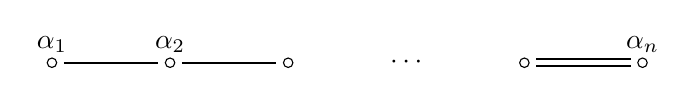
\begin{tikzpicture}[>=angle 90,scale=1.5]
\draw[] (0,0) circle(0.04) node[above]{$\alpha_1$};
\draw[] (1,0) circle(0.04) node[above]{$\alpha_2$};
\draw[] (5,0) circle(0.04) node[above]{$\alpha_n$};
\draw[] (4,0) circle(0.04);
\draw[] (2,0) circle(0.04);
\draw (3,0) node {$\cdots$};
\draw[thick] (0.1,0)  -- (0.9,0);
\draw[thick] (1.1,0) -- (1.9,0);
\draw[thick] (4.1,0.03) -- (4.9,0.03);
\draw[thick] (4.1,-0.03) -- (4.9,-0.03);
\end{tikzpicture}
\end{figure}


\noindent Recall that the positive roots have the form
$\gamma(k,\ell)\ {\dsize \mathrel{\mathop =^{def}}}\ \alpha_k + \alpha_{k+1} +\cdots + 
\alpha_\ell$ \quad  $\ell > k$\ or 
$\gamma^+(k,\ell)\ {\dsize \mathrel{\mathop =^{def}}}\ \alpha_k + \alpha_{k+1} +\cdots +
\alpha_{n-1} + \alpha_n + \alpha_{n-1} + \alpha_{n-1} + \cdots + \alpha_\ell$
\quad $\ell \ge k$.
Let ${\mathcal S}$  be the set of possibly empty pairs\ $(S_1,S_2)\subseteq
\Delta\times\Delta$, $S_1 = \{ \alpha_{i_1},\ldots ,\alpha_{i_p}\}$\ \quad 
$(i_1 < i_2 <\cdots < i_p)$,\ 
$S_2 = \{ \alpha_{j_1},\ldots ,\alpha_{j_q}\}  \quad (j_1 < \cdots < j_q)$
satisfying\ $i_p < j_1$\ and $j_q \ne n$.\ For each\ $(S_1,S_2)\in {\mathcal S}$\ we
define an open patch $Z_{(S_1,S_2)}$ of  $Z$  by

(i)\qquad $z(\alpha) \ne 0$ \quad if \quad $\alpha \notin S_1 \cup  S_2$ 
\quad	(write~~$z(\alpha_{i_k}) = z'_k \qquad z(\alpha_{j_k}) = z_k)$.

(ii)\quad $x(\alpha) \ne 0$~~if~~$\alpha\in S_1$

(iii)\quad $x_k\ {\dsize\mathrel{\mathop=^{def}}}\ x(\gamma(j_k,j_{k+1})) 
\ne 0 \qquad k\ne q$ 

\qquad\qquad~~~~$x_q\ {\dsize\mathrel{\mathop=^{def}}}\ 
x(\gamma^+(j_q,j_q)) \ne 0$.

(iv)\quad $w_k\ {\dsize\mathrel{\mathop=^{def}}}\ w(\gamma(j_k,j_{k+1}))\ne 0 
\qquad k\ne q$

\qquad\qquad~~~~$w_q\ {\dsize\mathrel{\mathop=^{def}}}\ w(\gamma^+(j_q,j_q))
\ne 0.$
\vskip .2in

\noindent Then on\ $Z_{(S_1,S_2)}$  if  $S_2\ne \emptyset$  we have by (3.7)
\vskip .2in

(i) \qquad  $w(\delta) = \dsize{\frac{x(\delta)w(\gamma)\Pi 
z(\alpha)^{m(\alpha)}}{x(\gamma)}}$

\qquad if  $x(\gamma)\ne 0$~~ and ~~ $\delta = \gamma + \Sigma m(\alpha)\alpha\quad 
m(\alpha) \ge 0$
\vskip .2in

(ii)\quad $x(\gamma) = \dsize{\frac{\lambda w(\gamma)}{\Pi z(\alpha)^{m(\alpha)}}}$
\qquad if~~$\gamma = \Sigma m(\alpha)\alpha \qquad \alpha \notin S_1 \cup S_2$
\vskip .2in

(iii)\quad $\lambda = \dsize{\frac{x_q}{w_q}} z^2_q(\Pi z(\alpha)^{m(\alpha)})
\qquad  2\alpha_{j_q} + \Sigma m(\alpha)\alpha = \gamma^+(j_q,j_q)$

%\pagebreak
\qquad (notice that~$x_q\ne 0, \Pi z(\alpha)^{m(\alpha)} \ne 0$,~~so~
$\lambda = 0$~~if and only if~~$z_q = 0$).
\vskip .2in

(iv)\quad $z_k = z_{k+2} \left( \dsize{\frac{x_{k+1}}{w_{k+1}}}{\frac{w_k}{x_k}}
{\frac{\Pi z(\alpha)^{m(\alpha)}}{\Pi z(\alpha)^{m'(\alpha)}}} \right)$

\quad where  $\Sigma m(\alpha)\alpha + \alpha_{j_{k+2}} = 
\gamma(j_{k+1},j_{k+2})$\ and\ $\alpha_{j_k} + \Sigma m'(\alpha)\alpha = \gamma(j_k,j_{k+1})$
\vskip .2in

\qquad \qquad~~~ $z_{q-1} = z_q \left( \dsize{\frac{w_{q-1}x_q\Pi 
z(\alpha)^{m(\alpha)}}{x_{q-1} w_q \Pi z(\alpha)^{m'(\alpha)}}} \right)$

where\qquad $2\alpha_{j_q} + \Sigma m(\alpha)\alpha =
\gamma^+(j_q,j_q)$\  and $\alpha_{j_{q-1}} + \alpha_{j_q} + \Sigma'm(\alpha)\alpha\
=\ \gamma(j_{q-1},j_q)$.
\vskip .2in

(v)\qquad $z'_\ell = \dsize{\frac{\lambda}{x(\alpha_\ell)}} = 
\dsize{\frac{x_q z^2_q(\Pi z(\alpha)^{m(\alpha)})}{w_qx(\alpha_\ell)}}$
~~where~~~ $2\alpha_{j_q} + \Sigma m(\alpha)\alpha = \gamma^+(j_q,j_q)$,
$\alpha_\ell \in S_1$.

Notice that (iv), (v) give  $z(\alpha) = f_\alpha z^\epsilon_q$\ for some  $f_\alpha$
regular and non-vanishing and\ $\epsilon\in \{ 0,1,2\}$.
\vskip .2in

(vi)\quad Suppose  $\gamma = \Sigma m(\alpha)\alpha$\ with\ $\Pi z(\alpha)^{m(\alpha)}
= f_\gamma z_q$, $f_\gamma$  regular and non-vanishing then
$$
x(\gamma) = \frac{x_qz_q(\Pi z(\alpha)^{m'(\alpha)})w(\gamma)}{f_\gamma},
\qquad 2\alpha_{j_q} + \Sigma m'(\alpha)\alpha = \gamma^+(j_q,j_q).
$$

\noindent $Z$ is defined by $p$ equations and is consequently $p+1$-dimensional.
A count of the equations in  $(i)\ldots (vi)$   reveals $p$ 
independent equations.  The coordinate ring being generated by the $p+1$
variables not appearing on the left hand side of $(i),\ldots ,(vi)$, 
we see that  $Z_{(S_1,S_2)}$ is regular, and that the divisor  $\lambda = 0$
on $Z_{(S_1,S_2)}$  has the form\ $(\lambda) = a(E_{(S_1,S_2)})E_{(S_1,S_2)}$\ 
with\ $a(E_{(S_1,S_2)}) = 2$\ where\ $E_{(S_1,S_2)}$\ is the prime divisor given
by  $z_q = 0$.

\begin{figure}[htb]
\centering
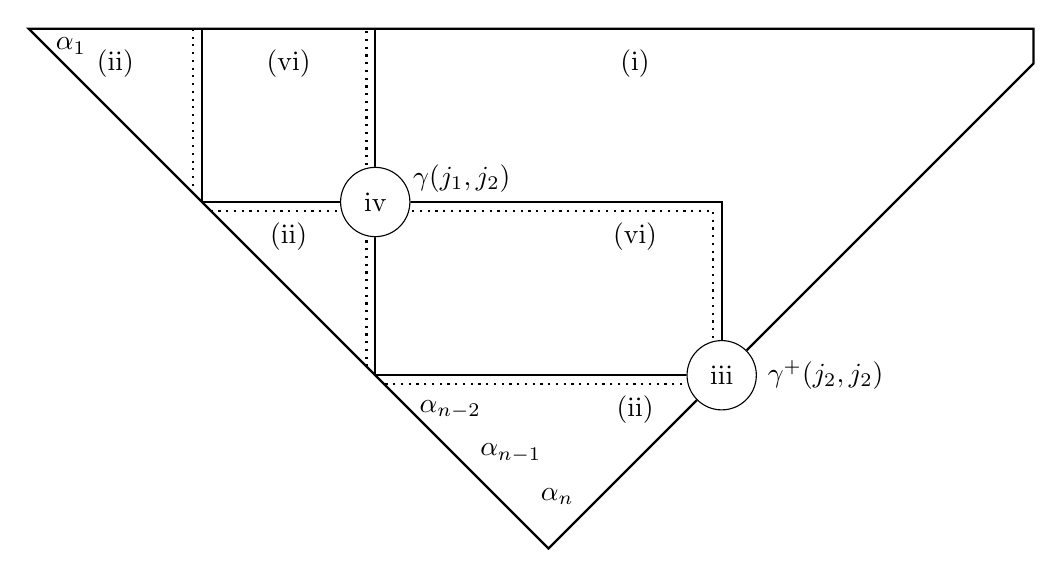
\begin{tikzpicture}[>=angle 90,scale=2.2]
\draw[thick] (3,0)--(6-0.2,3-0.2)--(6-0.2,3)--(0,3)--cycle;
\draw[thick] (1,3)--(1,2)--(4,2)--(4,1)--(2,1)--(2,3);
\draw[thick,dotted] (0.95,3)--(0.95,2+0.05);
\draw[thick,dotted] (1.05,2-0.05)--(4-0.05,2-0.05)--(4-0.05,1-0.05);
\draw[thick,dotted] (4-0.05,0.95)--(2+0.05,0.95);
\draw[thick,dotted] (2-0.05,1.05)--(2-0.05,3);
\draw (0.1,2.9) node[right]{$\alpha_1$};
\draw (2.2,0.8) node[right]{$\alpha_{n-2}$};
\draw (2.55,0.55) node[right]{$\alpha_{n-1}$};
\draw (2.9,0.3) node[right]{$\alpha_{n}$};
\draw (3.5,2.8) node {(i)};
\draw (0.5,2.8) node {(ii)};
\draw (1.5,2.8) node {(vi)};
\draw (1.5,1.8) node {(ii)};
\draw (3.5,1.8) node {(vi)};
\draw (3.5,0.8) node {(ii)};
\draw[fill,white] (2,2) circle (0.2);
\draw[fill,white] (4,1) circle (0.2);
\draw (2,2) circle (0.2);
\draw (4,1) circle (0.2);
\draw (2,2) node {iv};
\draw (4,1) node {iii};
\draw (4.6,1) node {$\gamma^+(j_2,j_2)$};
\draw (2.5,2) node[right,above] {$\gamma(j_1,j_2)$};
\end{tikzpicture}
\caption{{\noindent This diagram illustrates the $p$ equations for  $S_1 = \emptyset$ and
$|S_2| = 2$}}
\end{figure}


If  $S_2 = \emptyset$ then on $Z_{(S_1,\emptyset)}$\ we have by (3.7)


(i)\qquad  $w(\delta) = \dsize{\frac{x(\delta)w(\gamma)\Pi z(\alpha)^{m(\alpha)}}
{x(\gamma)}}$ if\ $x(\gamma)\ne 0$\ and\ $\delta = \gamma + \Sigma m(\alpha)\alpha \quad 
\alpha \ge 0$.
\vskip .2in

(ii)\quad $x(\gamma) = \dsize{\frac{\lambda w(\gamma)}{\Pi z(\alpha)^{m(\alpha)}}}
\qquad \qquad \gamma = \Sigma m(\alpha)\alpha \quad \alpha\notin S_1.$
\vskip .2in

(iii)\quad  $\lambda = z'_px(\alpha_{i_p}).$

(iv)\quad $z'_\ell = z'_p\left( \dsize{\frac{x(\alpha_{i_p})}{x(\alpha_{i_\ell})}}\right)
\qquad \ell\ne p\ \quad \alpha_{i_\ell} \in S_1.$
\vskip .2in

\noindent Again counting equations we see that\ $Z_{(S_1,\emptyset)}$\ is regular
and that the divisor $\lambda = 0$ on  $Z_{(S_1,\emptyset)}$\ has the form\
$(\lambda) = a(E_{(S_1,\emptyset)})E_{(S_1,\emptyset)}$\ with  $a(E_{(S_1,\emptyset)}) = 1$\
and\ $E_{(S_1,\emptyset)}$\ prime.

We extend the prime divisors  $E_{(S_1,S_2)}$\ to all of $Z$ by taking their
closures.

%\pagebreak
\proclaim{Lemma\ \ 4.2}\ (1)\ 
The codimension of the complement of $\dsize\bigcup_{(S_1,S_2)\in {\mathcal S}}
Z_{(S_1,S_2)}$\ in\ $Z$  is at least two.

\noindent %flushpar
(2)\ $Z$\ is regular in  codimension one.

\noindent %flushpar
(3)\ The divisor $(\lambda)$\ on $Z$ is given by
$$
(\lambda) = \sum_{(S_1,S_2)} a(E_{(S_1,S_2)})E_{(S_1,S_2)}
$$
$${\text{with}} \quad  a(E_{(S_1,S_2)}) =  \begin{cases}
1 & S_2 = \emptyset \\
2 & \text{otherwise.}
\end{cases}
$$
\endproclaim

\begin{proof}  By the preceding remarks (2) and (3) follow immediately from (1).
$Z$ is clearly regular for $\lambda\ne 0$\ so we study $\lambda$  near points
of  $\lambda = 0$.
%

Consider a point $p$ in $Z$ where $\lambda = 0$.  Let  $S_1$  be the set of simple
roots such that\ $x(\alpha)\ne 0$.  Let  $S_{\text{min}}$\  be the set of 
positive roots such that\ $x(\gamma)\ne 0$\ but if\ 
$\gamma = \beta + \Sigma m(\alpha)\alpha$,
$m(\alpha)\ge 0$\, $\alpha +\beta$, then\ $x(\beta) = 0$.\ Clearly\ $S_1\subseteq S_{\text{min}}$.
We may write\ $\Phi^+ = S_{\text{min}} \cup S^+ \cup S^-$, where
$S^+ = \{ \delta:  \delta = \gamma + \Sigma m(\alpha)\alpha \quad m(\alpha)\ge 0$
for some\  $\gamma \in S_{min}$,\ $\delta \notin S_{min}\}$.
$S^- = \{ \beta:  x(\beta) = 0 \}$.\ We have equations

(i)\qquad  $x(\beta) = 0 \qquad  \beta\in S^-$ 
\vskip .2in

(ii)\quad $w(\delta) = {\dsize\frac{w(\gamma)x(\delta)\Pi z(\alpha)^{m(\alpha)}}
{x(\gamma)}}$ \qquad $\delta  \in  S^+,~ \gamma\in S_{\text{min}}$,\  
$\delta  =  \gamma + \Sigma m(\alpha)\alpha\quad m(\alpha) \ge 0$.

%\bigpagebreak
\vskip .2in


(iii)\quad  if $\gamma = \gamma(k,\ell)$\ or\ $\gamma^+(k,\ell)
\in S_{\min}\backslash S_1$. 
$$
w(\gamma-\alpha_k)z(\alpha_k) = 
{\dsize{\frac{w(\gamma)x(\gamma-\alpha_k)}{x(\gamma)}}}
= 0 \qquad {\text{by the definition of}}~~ S_{\text{min}}
$$


(iv)\quad  $z(\alpha) = {\dsize{\frac{\lambda}{x(\alpha)}}} = 0~~{\text{if}}~~
\alpha\in S_1$

(v)\qquad   $\lambda = 0$.

\noindent %flushpar
Counting the number of equations we have at least  $p+1$  independent equations.
For the proof of (1)  we may exclude sets of codimension 2.  Thus we may assume that
(i)-(v)	 give exactly  $p+1$  independent solutions.  In particular, we may assume
that\ $S^-,S^+$\ and\ $S_{\text{min}}$\ are disjoint and that in (iii)  if\
$w(\gamma -\alpha_k) = 0$\ then\ $z(\alpha_k)\ne 0$.

Suppose that\ $\delta = \gamma(k,\ell)$\ or\ $\gamma^+(k,\ell) \in 
S_{\text{min}} \setminus S_1$,\ $\ell \ge k$.  Then as in (iii) we have\
$w(\delta -\alpha_\ell)z(\alpha_\ell) = 0$.  Suppose that\ $z(\alpha_\ell) \ne 0$.\
Then\ $w(\delta -\alpha_\ell) = 0$.\ This gives  $p+2$ equations unless
$\delta' = \gamma (k-1,\ell -1)\quad {\text{or}} \quad \gamma^+(k-1, \ell -1)
\in S_{\text{min}} \setminus S_1$\  
and the equation (iii) associated to  $\delta'$  is $w(\delta'- 
\alpha_{k-1}) = w(\delta - \alpha_\ell) = 0$  (and so
$z(\alpha_{k-1}) \ne 0)$.  But then
$$
w(\delta) = \frac{x(\delta) z(\alpha_{\ell})w(\delta')}{x(\delta')z(\alpha_{k-1})}
$$
gives  $p+2$ equations.  This contradiction shows that\ $z(\alpha_\ell) = 0$.

Now if\ $\gamma^+(r,\ell)\in S_{\text{min}}\setminus S_1$\  then\ $z(\alpha_\ell)
= 0$.\  This must be a consequence of (iii) so that\ $\gamma (\ell,m)$\ or\
$\gamma^+(\ell,m)\in S_{\text{min}}$.\  But this contradicts the definition of
$S_{\text{min}}$\ unless\ $r = \ell = m$.  Also by the definition of minimality there is
at most one $\ell$  such that\ $\gamma^+(\ell,\ell)\in S_{\text{min}} 
\setminus S_1$.\
Let\ $\gamma(j_1,j_2)\in S_{\text{min}} \setminus S_1$,\ then\ $z(\alpha_{j_2}) = 0$\
so there exists a\ $\gamma(j_2,j_3)$\ or\ $\gamma^+(j_1,j_2)\in S_{\text{min}}
\setminus S_1$.\  Continuing this way we obtain a chain\ 
$\gamma(j_1,j_2)$, $\gamma(j_2,j_3)\ldots \gamma^+(j_q,j_q)\in 
S_{\text{min}}\setminus S_1$,\
which we may assume to be maximal in length.  If also\ 
$\gamma(k_1,k_2)\in S_{\text{min}}\setminus S_1$\ we see that a 
new chain could be formed which must also end in\
$\gamma^+(k_{q'},k_{q'})$\ $k_{q'} = j_q$.\  But then\ 
$\kappa(b_{q'-1},k_{q'})$, 
$\gamma(j_{q-1},j_q)\in S_{\text{min}}\setminus S_1$\ and by 
the definition of\   $S_{min}$\, 
$\gamma(k_{q'-1},k_{q'}) = \gamma(j_{q-1},j_q)$.\ Continuing 
in this manner one finds that\ 
$\gamma(k_1,k_2) = \gamma(j_{q-q'+1},j_{q-q'+2})$.\ Thus
$\{ \gamma(j_1,j_2),\cdots \gamma^+(j_q,j_q)\} = 
S_{\text{min}} \setminus S_1\
{\dsize \mathrel{\mathop=^{def}}}\ S_2$.\  Since $\gamma^+(j_q,j_q)\notin
S_1$,\ $j_q\notin n$.\ Since (i)-(v) give all equations which
hold identically at $p$  (excluding sets of codimension 2) the inequalities 
defining\ $Z_{(S_1,S_2)}$\ hold at the generic point of the variety defined by
(i)-(v) together with\ $x(\gamma) \ne 0$, \quad $\gamma\in S_{min}$.
This completes the proof.\end{proof}

\vskip .2in

Turn to the case $G = C_2$.  We introduce new notation for thse divisors.  Set
$\alpha = \alpha_1$, $\beta = \alpha_2$.
\vskip .2in

\noindent (4.3)
$$
\begin{matrix} % \format \c & \quad \c &\quad \c & \qquad \qquad \l \\
\underline{S_1} & \underline{S_2} & \underline{E_{(S_1,S_2)}} & 
\underline{\pi(E_{(S_1,S_2)})} \\ \vspace{2\jot}
\{\alpha,\beta\} & \phi & E_0 & {\text{regular}} \\
\{\alpha\} & \phi & E_\beta & {\text{subregular}} \\
& & & {\text{Richardson~class~of}}~P_\beta \\
\{\beta\} & \phi & E_\alpha & {\text{subregular}} \\
& & & {\text{Richardson~class~of}}~P_\alpha \\
\phi & \{\alpha\} & E_2 & 2{\text{-regular}} \\
\phi & \phi & E_{id} & {\text{identity}}.
\end{matrix}
$$
\vskip .2in

\noindent The projection of each divisor to  $G$  is the closure of a stable
unipotent conjugacy class. The final column lists that conjugacy class.  
Write  $\gamma~ {\dsize \mathrel{\mathop=^{def}}}~ \alpha +\beta$, \quad 
$\delta = 2\alpha +\beta$. 
\vskip .2in

There are 4 stable unipotent classes in  Sp$(4)$ [Sp]:  the regular, the
subregular, the 2-regular and the 4-regular (the identity element).  For a
complete discussion see [Sp].  There is 
only one adjoint regular class, one adjoint 2-regular class, and one adjoint
4-regular class.  The adjoint subregular classes are in bijection with quadratic
extensions (or elements of  $F^\times/F^{\times 2})$.  To determine the quadratic extension
associated to a subregular unipotent element  $u\in G(F)$,   conjugate  $u$  by an
element of  $G(F)$  so that it has the form

$$
\begin{pmatrix} %\format \l \quad& \l \\
I_2 & X \\
0 & I_2 \end{pmatrix} 
\qquad \qquad \qquad I_2 = \begin{pmatrix} 1 & 0 \\ 0 & 1\end{pmatrix} \qquad
X\in M_2(F) ,
$$
where   Sp$(4)$  is defined using the skew form  $J_0 = \begin{pmatrix} 0 & J \\
-J & 0\end{pmatrix}$,\  $J = \begin{pmatrix} 0&1 \\ 1&0 \end{pmatrix}$.  Then %\linebreak
 $\det\, X \in
F^\times/F^{\times 2}$\  depends only on the adjoint conjugacy class of $u$.
Equivalently,  ${\mathcal B}_u$, the variety of Borel subgroups containing $u$, is a union of 
three projective lines.  The lines of type $\beta$  are defined over a 
quadratic extension of  $F$  depending only on the adjoint conjugacy class
of  $u$.

When  $G$  is the inner form of  Sp$(4)$  the regular, 2-regular, and 1-regular
adjoint class associated to the trivial quadratic extension 
$F^{\times 2} \subseteq F^\times/F^{\times 2})$\  do not exist.  If  $u\in G(F)$\ is unipotent
regular then there is a unique Borel subgroup over $F$  containing $u$.  If
$u\in G(F)$\ is 2-regular unipotent, then the line of type $\beta$ in
${\mathcal B}_u$  is defined over $F$  giving a parabolic of type $\beta$ over $F$;
but the minimal parabolic of  $G$  is of type $\alpha$.  If  $u\in G(F)$  is
1-regular corresponding to the trivial extension then the Borel subgroup
corresponding to the intersection of a line of type $\alpha$ and a line of type
$\beta$ in  ${\mathcal B}_u$  is defined over $F$.  Thus such unipotent classes do 
not exist for the inner form $G$.

\proclaim{Lemma\ \ 4.4}  (1)  The variety  $Z_\Phi \quad \Phi = C_2$  is regular
except possibly at points  $p$  such that  $\pi(p)$  is the identity element of
$G$  or at points  $p$  where 
$$
\lambda = x(\alpha) = x(\beta) = x(\gamma) = w(\gamma) = w(\delta) = 
z(\alpha) = z(\beta) = 0.
$$

\noindent % flushpar
(2)  The singularity at $\lambda = x(\alpha) = x(\beta) = x(\gamma) = w(\gamma)
= w(\delta) = z(\alpha) = z(\beta) = 0$  may be resolved by blowing up once along
the subvariety  $x(\alpha) = x(\beta) = x(\gamma) = w(\gamma) = w(\delta) =
z(\alpha) = z(\beta) = 0$.  Let  $E_B$  be the divisor introduced by blowing up.

\noindent %flushpar
(3)  The divisors on the desingularized variety and their Igusa constants are given
as follows (assume $\pi(p) \ne$ identity).
\endproclaim


$$
\begin{matrix} % \format \l & \qquad \c & \qquad \c & \qquad \c &\qquad \c   \\
\underline{E} & \underline{a(E)} & \underline{b(E)} & \underline{\pi(E)^\cdot}
& \underline{\beta(E)-1} \\
E_0 & 1 & 1 & 0{\text{-reg}} & 0 \\
E_\alpha & 1 & 2 & 1{\text{-reg}} & 1 \\
E_\beta & 1 & 2 & 1{\text{-reg}} & 1 \\
E_2 & 2 & 6 & 2{\text{-reg}} & 2 \\
E_B & 2 & 5 & 2{\text{-reg}} & 3/2
\end{matrix}
$$
\vskip .2in

\begin{proof}  The divisors $E_0,E_\alpha,E_\beta,E_{\text{id}}$\ are defined by

$E_0:  z(\alpha) = z(\beta) = w(\gamma) = w(\delta) = 0$

$E_\alpha:  x(\alpha) = z(\beta) = 0,  z(\alpha)w(\gamma) = w(\gamma)x(\beta),
w(\delta)x(\gamma) = w(\gamma)x(\delta)x(\alpha)$

$E_\beta:  x(\beta) = z(\alpha) = 0,  z(\beta)x(\gamma) = w(\gamma)x(\alpha), 
w(\delta) = 0$

$E_2:  z(\alpha) = x(\alpha) = x(\beta) = x(\gamma) = 0$

$E_{\text{id}}:  x(\alpha) = x(\beta) = x(\gamma) = x(\delta) = 0.$

\vskip .2in

\noindent %flushpar
We consider several patches, showing that the coordinate ring on each is regular,
and at the same time we identify the divisors on each patch. The defining relations
(3.7) of $Z$  are used repeatedly.

%\medpagebreak
\bigskip
\noindent %flushpar
(If   $x(\alpha) \ne 0) \qquad  \lambda = z(\beta)x(\beta)~~(E_0E_\beta) \quad
z(\alpha) = z(\beta)x(\beta)/x(\alpha),$ 

\noindent %flushpar
$w(\gamma) = x(\gamma)z(\beta)/x(\alpha),
w(\delta) = x(\delta)z(\alpha)z(\beta)/x(\alpha)$  

\noindent %flushpar
generators of local ring:
$z(\beta), x(\beta), x(\gamma), x(\delta), x(\alpha)$.

\bigskip
%\medpagebreak

\noindent %flushpar
(If   $x(\beta) \ne 0) \quad  \lambda = z(\alpha)x(\alpha) \quad (E_0E_\alpha)
\quad z(\beta) = z(\alpha)x(\alpha)/x(\beta),$  

\noindent %flushpar
$w(\gamma) = 
x(\gamma)z(\alpha)/x(\beta),  w(\delta) = x(\delta)z(\alpha)^2/x(\beta)$\

\noindent %flushpar
generators of local ring:\ $z(\alpha), x(\alpha), x(\beta), x(\gamma), x(\delta)$.

\bigskip
%\medpagebreak

\noindent %flushpar
(If  $x(\gamma) \ne 0$) $\lambda = x(\alpha)x(\beta) w(\gamma)/x(\gamma)$
$(E_\alpha E_0E_\beta)$,  $z(\alpha) = w(\gamma),x(\beta)/x(\gamma)$, 

\noindent %flushpar
$z(\beta) = w(\gamma)x(\alpha)/x(\gamma)$, $w(\delta) = w(\gamma)x(\delta)z(\alpha)/x(\gamma)$

\noindent %flushpar
generators:~  $x(\beta), x(\alpha), w(\gamma),x(\gamma), x(\delta)$.

\bigskip
%\medpagebreak

\noindent %flushpar
(If $z(\alpha)\ne 0$) $\lambda = z(\beta)x(\beta)$ $(E_\alpha E_{\text{id}})$
$x(\alpha) = z(\beta)x(\beta)/z(\alpha)$, 

\noindent %flushpar
$x(\gamma) = w(\gamma)x(\beta)/z(\alpha), x(\delta) = x(\beta)w(\delta)/z(\alpha)^2$,

\noindent %flushpar
generators:~  $x(\beta),z(\beta), w(\gamma), z(\alpha), w(\delta)$

\bigskip
%\medpagebreak

\noindent %flushpar
(If $w(\delta)\ne 0)$ $\lambda = 
z(\alpha)^2 z(\beta)x(\delta)/w(\delta)$ $(E^2_2E_\alpha E_{\text{id}})$

\noindent %flushpar
$x(\alpha) = z(\alpha)z(\beta)x(\delta)/w(\delta)$, $x(\beta) = 
z(\alpha)^2x(\delta)/w(\delta)$, $x(\gamma) = z(\alpha)w(\gamma)x(\delta)/w(\delta)$

\noindent %flushpar
generators:~$z(\alpha), z(\beta), x(\delta) w(\gamma), w(\delta)$
\vskip .2in

\noindent %flushpar
Since we are assuming  $\pi(p)\ne 1$  and since the variety has now been shown to be
nonsingular for  $x(\alpha), x(\beta)$  or  $x(\gamma)\ne 0$,  we may assume in 
the remaining cases that  $x(\delta)\ne 0$.

\bigskip
%\medpagebreak

\noindent %flushpar
(If  $w(\gamma)\ne 0$) $\lambda = x(\gamma)^2w(\delta)z(\beta)/(w(\gamma)^2x(\delta))$
$(E^2_2E_\beta E_\alpha)$ 

\noindent %flushpar
$z(\alpha) = w(\delta)x(\gamma)/(w(\gamma)x(\delta))$,
$x(\alpha) = z(\beta)x(\gamma)/w(\gamma)$,\ $x(\beta) = 
x(\gamma)^2w(\delta)/(w(\gamma)^2x(\delta))$

\noindent %flushpar
generators:~ $x(\gamma),x(\delta),z(\beta),w(\gamma),w(\delta)$.

\bigskip
%\medpagebreak

\noindent %flushpar
(If  $z(\beta) \ne 0)$ $\lambda = w(\delta)x(\alpha)^2/(z(\beta)x(\delta))$ $(E_\beta E^2_2)$ 
$x(\beta) = w(\delta)x(\alpha)^2/(z(\beta)^2x(\delta))$,  

\noindent %flushpar
$x(\gamma) =
w(\gamma)x(\alpha)/z(\beta)$, $z(\alpha) = w(\delta)x(\alpha)/(x(\delta)z(\beta))$~

\noindent %flushpar
generators:~ $x(\alpha), x(\delta), z(\beta), w(\gamma), w(\delta)$.

\vskip .2in

\noindent %flushpar
This completes the proof of (1).  The validity of (2) is easily checked using the
same seven patches.  Details are omitted.

The only points that are not clear in (3) are the value of the constants
$b(E)$ and the value of  $a(E_B)$.  $b(E)-1$  is given as the order to which the
form (3.8)
$$
\omega_Y = d\lambda dx(\alpha) dx(\beta) dx(\gamma) dx(\delta) dv
$$
$$
dv = dv(\alpha) dv(\beta) dv(\gamma) dv(\delta)
$$
vanishes along $E$.  For example, the form when expressed in terms of the coordinates
on the path  $(w(\gamma)\ne 0)$\  becomes
$$
\omega_Y = x(\gamma)^5w(\delta)z(\beta)/(x(\delta)^2w(\gamma)^4)dz(\beta)
d(1/w(\gamma))dw(\delta)dx(\delta)dv\quad 
(E_2^{6-1}E_\beta^{2-1}E_\alpha^{2-1)}.
$$

\noindent %flushpar
Thus   $b(E_2) = 6, b(E_\beta) = 2, b(E_\alpha) = 2$.  The Igusa constants
$b(E)$  for  $E = E_B,E_0$  are similarly calculated using a blown up region.
Introduce projective coordinates  $X_\alpha,X_\beta,X_\gamma,Z_\alpha,W_\delta,Z_\beta,W_\gamma$.
On  $X_\alpha = 1$  we have  $X_\beta x(\alpha) = x(\beta)$, $X_\gamma x(\alpha) =
x(\gamma)$.\   The patch $(x(\alpha)\ne 0)$\ becomes (dropping 
the assumption that  $x(\alpha)\ne 0$).
$$
\lambda = x(\alpha)^2 Z_\beta X_\beta ~~ (E^2_BE_0E_\beta)~~Z_\alpha = Z_\beta X_\beta,~~
W_\gamma = X_\gamma Z_\beta ,
$$
$$
W_\delta = x(\delta)Z_\alpha Z_\beta~~{\text{so~that}}~~ a(E_B) = 2.
$$
$$
\omega_Y = x(\alpha)^{5-1}Z_\beta^{1-1}X_\beta^{2-1} dZ_\beta dx(\alpha)dX_\beta
dX_\gamma dx(\delta)dv
$$
$$
{\text{so~that}}~~b(E_B) = 5,~~ b(E_0) = 1,~~ b(E_\beta) = 2 .
$$
This completes the proof.\end{proof}

%5
\section{The subregular germs on $G =$~Sp(4)}

\vskip .2in

We begin with a summary of the results of this section.  Let  $G$  be Sp(4) or
its inner form.  By (2.5) we will have determined all of the germs of\
$GSp(4)$\ once we have calculated those of\ $Sp(4)$.\  Details on 
normalizations of measures are found below.  Let
$\alpha'$  be a root of Sp(4), let  $E$  be a quadratic extension (possibly
trivial of $F$), and let  $H$  be an endoscopic group.  Let  $T(\alpha')$  be a Cartan
subgroup corresponding to the homomorphism  Gal$(\overline{F}/F) \to W$  given
by  $\sigma\in$ Gal$(E/F)$\ $(\sigma\ne 1)$\  $\sigma \mapsto \sigma_{\alpha'}\in W$
(or let  $T(\alpha')$  be split if  $E = F$).

Let  $O_{E'}$\ be the subregular adjoint unipotent class associated to the 
quadratic extension\ $E'$\ of  $F$\  (see discussion following 4.3).  Let
$\Gamma(E',E,\alpha')$\  be the germ of\ $O_{E'}$\ for the pair $(T(\alpha'),st)$\
where $st$  is the trivial character on\ $H^1(Gal(\overline{F}/F), T(\alpha'))$.
Set\ $\Gamma(E',E,\alpha') = 0$\ if  $T(\alpha')$  does not exist.  The function
$\Gamma_1(E',E'',\beta)$\
is defined in (5.18).  Set\ $\delta_G = 1$\ if $G$ is quasi-split, $0$ otherwise;
set  ${\epsilon}_G = 2\delta_G-1$; and set\ $\delta(E,E') = 1$\ if $E = E'$,
$0$ otherwise.  Then we have for various  $(T,\kappa)$ in $G$  associated to
endoscopic groups\ $H$\ (4.1)

\noindent (5.1)
$$
\begin{matrix} % \format \l & \qquad\l & \qquad\l & \quad\l \\
\underline{H} & \underline{T} & \underline{{\text{Germ~of}}~O_{E'}\ E'\ne F}  
& \underline{{\text{Germ~of}}~O_F}   \\  \vspace{2\jot}
{}^{E}{H_1}\ E\ne F & U_{E''}(1)\times U_E(1) & \delta(E,E')\delta_G\Gamma_1(E',E'',\beta)
& 0 \\
\vspace{1.5\jot}
{}^{E}{H_2}\ E\ne F & arbitrary & 0 & 0 \\
\vspace{1.5\jot}
{}^F{H_0} & T/(\pm 1) =  & \Gamma(E',E,\alpha)
& \Gamma(F,E,\alpha) \\
\vspace{1.5\jot}
{} & \qquad U_{E''}(1)\times U_E(1) & \qquad +\epsilon_G\Gamma(E',E'',\gamma) &
\qquad +\epsilon_G\Gamma(F,E'',\gamma) \\
\vspace {1.5\jot}
{}^F{H_2} & arbitrary & {\epsilon}_G\Gamma_{O_{E'}}^{T_{qs},st} & 
\delta_G \Gamma_{O_F}^{T_{qs},st} .
\end{matrix}
$$
\vskip .2in
		     
Quasi-split reduction will be useful in identifying the germs of the subregular 
unipotent classes.  For a group of semi-simple rank 2, quasi-split reduction is a 
statement about the matching of inner forms of rank 1 groups.  This situation
is well understood.  See for example [LS].  In particular it follows immediately
from the well know matching of orbital integrals on a rank 1 group with orbital
integrals on its quasi-split inner form that G has quasi-split reduction.

The variety of Borel subgroups containing a given subregular unipotent element in a
group of type  $C_2$  is a union of three projective lines and is called the
Dynkin curve.  There is one line corresponding to the short root and two lines
corresponding to the long root.  If  $u$  is contained in  $G(F)$  then
Gal$(\overline{F}/F)$\ permutes the lines  $\ell_\beta , \ell'_\beta$  corresponding
to the long root.  We say that a subregular class is distinguished if the quadratic extension associated
to it is the trivial extension, that is, all three lines are defined over  $F$. 
Most of the analysis of this section will be devoted to the classes which are not
distinguished.

\proclaim{Lemma\ \ 5.2}  Suppose that  $H$  is an endoscopic group of $G$ which is
split by a nontrivial quadratic extension  $E$ of $F$.  Let  $(T,\kappa)$     be a
pair associated to  $H$.  Then the subregular germ of the unipotent class  $O_{E'}$
associated to the quadratic extension  $E'$  for the pair  $(T,\kappa)$  is zero
unless $E' = E$.
\endproclaim

\begin{proof} Let $Z$ be the center of $G$.  Let $u \in O(F)$ and let $C_G(u)_{red}$
be the reductive centralizer of $u$.
If  $\kappa$  is nontrivial on  ker$(H^1(Gal(\overline{F}/F),Z)\to 
H^1(Gal(\overline{F}/F),  C_G(u)_{red}))$\
pick  $h$
so that  $O^h = O$, $\kappa(\sigma(h)h^{-1})\ne 1$  so that by (2.1)\
$\Gamma_O^{T,\kappa} = 0$. It was mentioned in (2.1) that $\kappa$ restricted to
$H^1(Gal(\overline{F}/F, Z)$\ depends only on the endoscopic group associated to
to  $(T,\kappa)$.  We see this directly as follows in the case that  $G$  is the 
inner form of a split group and  $Z = \{\pm 1\}$   and  $H$  split by a quadratic
extension $E$ of  $F$.  Directly from the definition of endoscopic groups we 
see easily that  $E = F$  if and only if  $H$ (up to a central factor) is an 
endoscopic group of  $G$  which in turn is true if and only if  $\kappa$ 
restricted to\ $H^1(Gal(\overline{F}/F), Z)$\ is trivial.  If  $E$  is a 
nontrivial extension then  $\kappa$ is nontrivial but trivial over the 
quadratic extension $E$ of $F$.  In other words,     $\kappa$ is trivial on the
image of the corestriction map from\ $H^1(Gal(\overline{F}/E), Z)$\ to
$H^1(Gal(\overline{F}/F, Z)$.  Identifying  $H^1(Gal(\overline{F}/F), Z)$ with
$F^\times/F^{\times 2}$\ it follows that  $\kappa$  may be identified with the
nontrivial character on  $F^\times/NE$\ where  $NE$  is by definition the group
of norms of nonzero elements of  $E$.  To complete the proof it is sufficient
to show that  ker$(H^1(Gal(\overline{F}/F),Z) \to H^1(Gal(\overline{F}/F),\
C_G(u)_{red}))$\ is\ $NE'/F^{\times 2} \subseteq F^\times/F^{\times 2}$. 

The reductive centralizer is computed when  $G$  is split as follows.  
Let  $B$  be a Borel subgroup over
$F$  in the line of type $\alpha$  in the Dynkin curve of $u$.  Conjugating $B$
to the upper triangular matrices we see that
$$
u = \begin{pmatrix} I_2 & XJ \\
0 & I_2
\end{pmatrix}
$$
where  $X = {}^tX \in {\text{GL}}_2(F)$\ and  $J = \begin{pmatrix} 0&1 \\ 1&0 \end{pmatrix}$.  It
follows immediately that  
$$
C_G(u) = \begin{pmatrix} {}^tA & B \\ 0 & JA^{-1}J \end{pmatrix}\
\quad {\text{and}}\quad  C_G (u)_{\text{red}} = 
\begin{pmatrix} {}^tA & 0 \\ 0 & JA^{-1}J \end{pmatrix}
$$
where  ${}^tAXA = X$.  Thus\  $C_G(u)_{\text{red}}\ 
{\dsize \mathrel{\mathop \to^{\sim}}}\
U_{E'}(1)$\  a one dimensional torus split by  $E'$.\ $ker(H^1(Z) \to
H^1(C_G(u)_{\text{red}}))$\ is then identified with $NE'/F^{\times 2} \subseteq F^\times /F^{\times 2}$\  and the lemma follows for $G$
split.

When  $G$  is not split we make the following modifications.  $G$  contains a parabolic
subgroup  $P_\alpha$  over  $F$  which is identified modulo a Borel subgroup 
$B$  with the line of
type $\alpha$  in the Dynkin curve of $u$.  Thus we may assume that  $u$  has the
same form.  Over the quadratic extension  $E'$  of  $F$~~ $G$ splits and $u$
becomes distinguished so that over  $E'$\ it follows that $C_G(u)_{\text{red}}~
{\dsize \mathrel{\mathop\to^{\sim}}}\ {\bold G}_m$.  But if  $C_G(u)_{\text{red}}$\
were isomorphic to  ${\bold G}_m$  over  $F$  we would have a split torus in
$\begin{pmatrix} {}^tM & 0 \\ 0 & JM^{-1}J \end{pmatrix}$,\ \ where $det~M = 1$,  which would
contradict the hypothesis that  $G$ is not split.  Thus\ $C_G(u)_{\text{red}}\
{\dsize \mathrel{\mathop\to^{\sim}}}\ U_{E'}(1)$\  as before, and  $E' \ne F$. 
This completes the proof of (5.2).
\end{proof}
\bigskip

We have seen there are two divisors which contribute to the subregular germ.  
On the patch  $Y_U$   given by (3.7)
\begin{align*}
\lambda &= z(\alpha)x(\alpha)\\
\lambda &= z(\beta)x(\beta)\\
\lambda w(\gamma) &= z(\alpha)z(\beta)x(\gamma) \\
\lambda w(\delta) &= z(\alpha)^2z(\beta)x(\delta).
\end{align*}
$E_\alpha$  is described by the equations\ $x(\alpha) = z(\beta) = x(\beta)w(\gamma) 
- z(\alpha)x(\gamma) = x(\beta)w(\delta) - z(\alpha)^2x(\delta) = 0$\ and  $E_\beta$\
is described by the equations\ $x(\beta) = z(\alpha) = w(\delta) = x(\alpha)w(\gamma)
- z(\beta)x(\gamma) = 0$.

\proclaim{Lemma\ \  5.3}  If  $u_0$  is not distinguished then  $E_\beta$  contains no
$F$-rational points over  $u_0$  and consequently makes no contribution to the
germ associated to  $u_0$.
\endproclaim

\begin{proof}  The lemma is an immediate consequence of two facts.  First, if
$(u_0, (B(W))) \in E_\beta$\  then every Borel subgroup  $B(W)$  lies in the same
line  $\ell_\beta$  of type $\beta$  in the Dynkin curve.  For select local
coordinates as in (3.12) such that  $B_0$  lies in  $\ell_\beta$  and  $\ell_\beta$  contains
$B(W_+)$.  Then  $B(W) = B_0^{n_Wv}$\  where  $n_W$  has the form
\begin{equation}
n_W = \exp(z(\alpha)z_kX_{-\alpha})\exp(z(\beta)z_{k-1}X_{-\beta})\cdots 
\exp(z(\alpha)z_1X_{-\alpha}) \tag {5.4}
\end{equation}
for appropriate values of\ $z_1,\ldots ,z_k$.  So  $z(\alpha) = 0$\   implies that
the product (5.4) collapses to\ $n_W = \exp(z(\beta)z'X_{-\beta})$\  
for some  $z'$.  Also\ $B_0^v = B(W_+)\in \ell_\beta$\  
and\ $B_0,\quad B(W_+)\subseteq P_\beta$\ where\
$B\backslash P_\beta = \ell_\beta$\  so\  $P_\beta^v = P_\beta$\  
which implies that\  $v\in N_\infty \cap P_\beta$\  or 
$v = \exp(\xi\ X_{-\beta})$\  for some $\xi$, where  $N_\infty$ is the unipotent
radical of  $B_\infty$.  Thus  $n_wv\in P_\beta$\  and  $B(w) = B_0^{n_wv} \in P_\beta$.  Thus
if $\ell_\beta$ and $\ell'_\beta$  are the lines of the Dynkin curve of  $u_0$
we may separate points $(u_0, (B(W)))$\ of $E_\beta$ 
into $\ell_\beta$-points and  $\ell'_\beta$-points according to where the Borel
subgroups lie.  Second, the action of  Gal$(\overline{F}/F)$\ on the points of
$E_\beta$  interchanges  $\ell_\beta$-points with $\ell'_\beta$-points.  For the
action (3.13) is given by\ $(u_0, (B(W))) \mapsto (u_0, (\sigma(B(\sigma_T^{-1}W))))$\
for $\sigma\in Gal(\overline{F}/F),~ u_0\in G(F)$.\  If  $B(W)$\ lies in  $\ell_\beta$
then  $B(\sigma_T^{-1}W)$\  lies in  $\ell_\beta$  and  $\sigma(B(\sigma_T^{-1}W))$\
lies in\  $\sigma(\ell_\beta) = \ell'_\beta$\  provided $\sigma$  has nontrivial
image in  Gal$(E/F)$\  where  $E$  is the quadratic extension trivializing the
action on the lines  $\ell_\beta, \ell'_\beta$.
\end{proof}
\vskip .2in

We now devote our attention to the divisor  $E_\alpha$.  We fix  $u_0$  a subregular
element which is not distinguished and let  $B_0$  be a Borel subgroup at the
intersection of the line of type $\alpha$  and a line of type $\beta$ in the
Dynkin curve of  $u_0$.   As in the discussion of the divisor  $E_\beta$  we find that
if  $(u, B_0^{n_W})^v$\  lies in  $E_\alpha$  over the subregular element
$u_0$  then  $u^v = u_0$\  and  $v\in P_\alpha \cap N_\infty$\  so that\
$v = \exp(\xi X_{-\alpha})$\  for some  $\xi$.

Select a Cartan subgroup\  $T_0\subseteq B_0$\  over  $F$  such that if
$\sigma_\alpha$\  is the simple reflection associated to the simple root $\alpha$,
\quad $B_0^{\sigma_\alpha}$\  is equal to the Borel subgroup at the intersection of
$\ell_\alpha$  and  $\ell'_\beta$\ (the second line of type $\beta$ in the
Dynkin    curve). Such a Cartan subgroup may be found by selecting any Cartan over
$F$  in  $B_0$  and in a Levi factor over  $F$  of  $P_\alpha$      where  
$B\setminus P_\alpha =   \ell_\alpha$.\ Let  $B_\infty$  be the Borel subgroup
opposite  $B_0$  through  $T_0$.  We consider the patch\ $Y_U = Y_U(B_\infty,B_0)$\
for this choice of  $(B_\infty, B_0)$.

The choice of  $B_0$  forces  $u_0$  to have the form 
$u_0 = \begin{pmatrix} I_2 & X \\ 0 & I_2 \end{pmatrix}$, 
\quad  $X = \begin{pmatrix} x&y\\ 0&x \end{pmatrix} .$\  The choice of  $B_\infty$  
forces\ $\sigma_\alpha u_0\sigma_\alpha^{-1}$\ to have the
same form which implies that  $y = 0$  so that
\begin{equation}
u_0 = \begin{pmatrix} I_2 & xI_2 \\ 0 & I_2 \end{pmatrix} \tag {5.5}
\end{equation}

We choose a Haar measure on  $O_{u_0}$  as follows.  We select coordinates
$v' = \begin{pmatrix} I_2 & 0 \\ N&I_2 \end{pmatrix}$, \quad $y =
\begin{pmatrix} I_2 & Y \\ 0 & I_2 \end{pmatrix}$,\ 
$N = \begin{pmatrix} n_\gamma & n_\beta \\ n_\delta & n_\gamma \end{pmatrix} ,$\
 \quad
$Y = \begin{pmatrix} y_\gamma & y_\delta \\ y_\beta & y_\gamma \end{pmatrix}$\
so that  $y^{v'}$  describes points on an open set of  $O_{u_0}$.
Then  
\begin{equation}
{\frac{1}{2}}\ dy\ dv'\ {\mathrel{\mathop=^{def}}}\ {\frac{1}{2}}\
dy_\beta dy_\gamma dy_\delta dn_\beta dn_\gamma dn_\delta    \tag {5.6}
\end{equation}
is an invariant measure on\  $O_{u_0}$.

We consider the patch  $x(\gamma) \ne 0$  on  $Y_U$\  so that the
equations (3.7) take the form
\begin{equation}
\lambda = {\frac{x(\alpha)x(\beta)w(\gamma)}{x(\gamma)}}, \quad 
z(\alpha) = {\frac{x(\beta)w(\gamma)}{x(\gamma)}}, \quad 
z(\beta) = {\frac{x(\alpha)w(\gamma)}{x(\gamma)}}, \quad
w(\delta) = {\frac{x(\beta)w(\gamma)^2x(\delta)}{x(\gamma)^2}}
\tag {5.7}
\end{equation}
%\pagebreak
\noindent
By (1.1), (3.8), and a change of variables
$$
\omega_{E_\alpha} = {\frac{x(\gamma)}{x(\beta)}}\ {\frac{dw(\gamma)}{w(\gamma)^2}}\
dx(\beta)dx(\gamma)dx(\delta)dv = {\frac{\omega_Y}{\lambda^2{\frac{dx(\alpha)}
{x(\alpha)}}}} .
$$
We divide by the Haar measure  $\omega_{O_{u_0}} = (1/2)dx\ dv' =  (1/2)dy\ dv'$\
$(dx = dx(\beta)\ dx(\gamma)\ dx(\delta))$
to obtain a differential form\ $\omega_{E_\alpha(u_0)}$\ on the fibre  
$E_\alpha(u_0)$ over  $u_0$.  Making
use of the fact that  $v = \exp(\xi X_{-\alpha})$\ on  $E_\alpha(u_0)$\  this gives
\begin{equation}
\omega_{E_\alpha(u_0)} = {\frac{2x(\gamma)}{x(\beta)}}\ {\frac{dx}{w^2}} d\xi
\qquad \qquad  w = w(\gamma).
\tag {5.8}
\end{equation}

Next we note that if  $(u, B(w))^v$  is a point of  $E_\alpha(u_0)$\
with  coefficients $x_\beta(u) = x(\beta) \quad x_\gamma(u) = x(\gamma), ~x_\delta(u) =
x(\delta)$\ we must have  $u^v = u_0$\ with $v = \exp(\xi X_{-\alpha})$.
By (5.5) this implies that  $x(\delta) = 0$,  and $x(\gamma)/x(\beta)
= 1/2\xi$\  so that (5.8) becomes
\begin{equation}
\omega_{E_\alpha(u_0)} = {\frac{dw}{w^2}}\ {\frac{d\xi}{\xi}}  \tag {5.9}
\end{equation}
Note that it is always possible to recover the action of  Gal$(\overline{F}/F)$\
from the action of  $W\times A$  and the action  $\sigma_*$  for a split Cartan
subgroup and  $B_0$  over  $F$.\  The equation\ $\sigma_{\alpha'}(x_\gamma(b)) =
x_\gamma(b')$\  of (3.13) gives for an {\it arbitrary} divisor.
\vskip .2in
\noindent (5.10)
\begin{enumerate}[label=]
\item{}\qquad  $\sigma_\alpha(x(\alpha))/x(\alpha)\ =\ 1$
\item{}\qquad  $\sigma_\alpha(x(\beta))/x(\beta)\ =\ 1+2(T_1-T_2)w(\gamma) +
(T_1-T_2)^2w(\delta)$
\item{}\qquad $\sigma_\alpha(x(\gamma))/x(\gamma)\ =\ 1+(T_1-T_2) 
z(\alpha)x(\delta)/x(\gamma)\ =\ 1 + (T_1-T_2) 
w(\delta)/w(\gamma)$
\item{}\qquad $\sigma_\alpha(x(\delta))/x(\delta)\ =\ 1$
\vskip .3in

\item{}\qquad $\sigma_\beta(x(\alpha))/x(\alpha)\ =\ 1 - 2T_2w(\gamma)$
\item{}\qquad $\sigma_\beta(x(\beta))/x(\beta)\ =\ 1$
\item{}\qquad $\sigma_\beta(x(\gamma))/x(\gamma)\ =\ 1$
\item{}\qquad $\sigma_\beta(x(\delta))/x(\delta)\ =\ 1$.
\end{enumerate}
\vskip .2in
\noindent Here $T_1,\ T_2$ represents the tangent direction of the curve
$\Gamma$ in $T$ at the identity and $\sigma_\alpha$ and $\sigma_\beta$ are simple
reflections associated to the simple roots $\alpha$ and $\beta$.
From the choice of  $B_0$  made following lemma 5.3 the image of the group $A$ in the 
Weyl group is the
subgroup     of order two generated by the reflection  $\sigma_\alpha$.  Let
$\sigma_0$  be the representative of\ $\sigma_\alpha$\ in  $A$.  Then  
(3.13) and (5.10) 
specializing to
the divisor  $E_\alpha$  give
\begin{align*}
\sigma_\beta(\xi) &= \xi  \tag {5.11} \\
\sigma_\alpha(\xi) &= 1/\zeta \xi \\
\sigma_\beta(w) &= w/(-2T_2w+1) = w/w_B \\
\sigma_\alpha(w) &= w/w_A \\
\sigma_0(w) &= -w/w_A 
\end{align*}
where we introduce abbreviations
\begin{align*}
w_A &= (T_1-T_2)w + 1 \tag {5.12} \\
w_B &= -2T_2w + 1 \\
w_D &= 2T_1w + 1 .
\end{align*}
and $\zeta$\ is an element of  $F^\times$.  Since  $\sigma_0,\sigma_\alpha$ and $\sigma_\beta$  
generate  $W\times A$ we easily
deduce the following charts:
\noindent (5.13)
$$
\begin{matrix} 
% \format \c\quad & \c\quad & \c\quad  & \c\quad &\c\quad & \c\quad  & \c\quad \\
\underline{\sigma} & \underline{\sigma(w)} & \underline{\sigma(w_A)} &
\underline{\sigma(w_B)} & \underline{\sigma(w_D)} & \underline{\sigma(\xi)}
& \underline{t_\sigma} \\
\vspace{2\jot}
1 & w & w_A & w_B & w_D & \xi & (1,1) \\
\vspace{1.5\jot}
\sigma_\alpha & {\dsize\frac{w}{w_A}} & {\dsize\frac{1}{w_A}} & {\dsize\frac{w_B}{w_A}} & 
{\dsize\frac{w_D}{w_A}} &  w_A\xi & (\xi w,\ {\dsize\frac{1}{\xi w}}) \\
\vspace{1.5\jot}
\sigma_\beta\sigma_\alpha & {\dsize\frac{w}{w_D}} & {\dsize\frac{w_B}{w_D}} & {\dsize\frac{1}{w_D}}
& {\dsize\frac{w_A}{w_D}} & {\dsize\frac{w_D\xi}{w_B}} & ( {\dsize\frac{\xi w}{w_B}},\ 
{\dsize\frac{-w}{w_Bx(\gamma)}})\\
\vspace{1.5\jot}
\sigma_\alpha\sigma_\beta\sigma_\alpha & {\dsize\frac{w}{w_D}} & {\dsize\frac{w_B}{w_D}} &
{\dsize\frac{w_A}{w_D}} & {\dsize\frac{1}{w_D}} & {\dsize\frac{w_Aw_D\xi}{w_B}} &
({\dsize\frac{\xi w^2}{w_Bx(\gamma)}},\ {\dsize\frac{w_A}{w_B}})\\
\vspace{1.5\jot}
\sigma_\alpha\sigma_\beta\sigma_\alpha\sigma_\beta & {\dsize\frac{w}{w_A}} & 
{\dsize\frac{1}{w_A}} & {\dsize\frac{w_D}{w_A}} & {\dsize\frac{w_B}{w_A}} & 
{\dsize\frac{w_Aw_D\xi}{w_B}} & ({\dsize\frac{-w^2\xi}{w_Bx(\gamma)}},\ 
{\dsize\frac{-1}{x(\gamma)w_D\xi}}) \\
\vspace{1.5\jot}
\sigma_\beta\sigma_\alpha\sigma_\beta & w & w_A  & w_D & w_B &
{\dsize\frac{w_D\xi}{w_B}} & ({\dsize\frac{-w}{w_Dx(\gamma)}},\ {\dsize\frac{-w}{w_Bx(\gamma)}})\\
\vspace{1.5\jot}
\sigma_\alpha\sigma_\beta & {\dsize\frac{w}{w_B}} & {\dsize\frac{w_D}{w_B}} & {\dsize\frac{w_A}{w_B}}
& {\dsize\frac{1}{w_B}} & w_A\xi & ({\dsize\frac{w}{w_Ax(\gamma)}},\ {\dsize\frac{1}{\xi w}}) \\
\vspace{1.5\jot}
\sigma_\beta & {\dsize\frac{w}{w_B}} & {\dsize\frac{w_D}{w_B}} & {\dsize\frac{1}{w_B}} &
{\dsize\frac{w_A}{w_B}} & \xi & (1,\ {\dsize\frac{1}{\xi x(\gamma)}} ) 
\end{matrix}
$$

\noindent (5.13)  (cont.)
$$
\begin{matrix}
%\format \c\quad & \c\quad & \c\quad  & \c\quad &\c\quad 
& \c\quad  & \c\quad \\
\underline{\sigma} & \underline{\sigma(w)} & \underline{\sigma(w_A)} &
\underline{\sigma(w_B)} & \underline{\sigma(w_D)} & \underline{\sigma(\xi)}
& \underline{t_\sigma} \\
\vspace{2\jot}
\sigma_0 & {\dsize\frac{-w}{w_A}} & {\dsize\frac{1}{w_A}} & {\dsize\frac{w_D}{w_A}} &
{\dsize\frac{w_B}{w_A}} & {\dsize\frac{1}{\zeta\xi}} & (\xi, \xi^{-1}) \\
\vspace{1.5\jot}
\sigma_\alpha\sigma_0 & -w & w_A  & w_D & w_B & {\dsize\frac{1}{\zeta w_A\xi}} &
({\dsize\frac{w}{w_A}}, {\dsize\frac{w_A}{w}}) \\
\vspace{1.5\jot}
\sigma_\beta\sigma_\alpha\sigma_0 & {\dsize\frac{-w}{w_B}} & {\dsize\frac{w_D}{w_B}} &
{\dsize\frac{w_A}{w_B}} & {\dsize\frac{1}{w_B}} & {\dsize\frac{w_B}{(\zeta w_D\xi)}} &
({\dsize\frac{w}{w_D}},\ {\dsize\frac{w}{w_D}}\xi) \\
\vspace{1.5\jot}
\sigma_\alpha\sigma_\beta\sigma_\alpha\sigma_0 & {\dsize\frac{-w}{w_B}} & {\dsize\frac{w_D}{w_B}}
& {\dsize\frac{1}{w_B}} & {\dsize\frac{w_A}{w_B}} & {\dsize\frac{w_B}{(\zeta w_Aw_D\xi)}} &
({\dsize\frac{w^2}{w_Aw_D}},\ {\dsize\frac{-1}{w_D\xi}}) \\
\vspace{1.5\jot}
\sigma_\alpha\sigma_\beta\sigma_\alpha\sigma_\beta\sigma_0 & -w & w_A & w_B & w_D &
{\dsize\frac{w_B}{(\zeta w_Aw_D\xi)}} & ({\dsize\frac{w^2}{w_Aw_D}},\ {\dsize\frac{w_A}{x(\gamma)w_B}}) \\
\vspace{1.5\jot}
\sigma_\beta\sigma_\alpha\sigma_\beta\sigma_0 & {\dsize\frac{-w}{w_A}} & {\dsize\frac{1}{w_A}}
& {\dsize\frac{w_B}{w_A}} & {\dsize\frac{w_D}{w_A}} & {\dsize\frac{w_B}{(\zeta w_D\xi)}} &
({\dsize\frac{w\xi}{x(\gamma)w_B}},\ {\dsize\frac{w}{w_Dx(\gamma)\xi}}) \\
\vspace{1.5\jot}
\sigma_\alpha\sigma_\beta\sigma_0 & {\dsize\frac{-w}{w_D}} & {\dsize\frac{w_B}{w_D}} & {\dsize\frac{1}{w_D}}
& {\dsize\frac{w_A}{w_D}} & {\dsize\frac{1}{(\zeta w_A\xi)}} & ({\dsize\frac{w\xi}{x(\gamma)}},\ 
{\dsize\frac{w_A}{w}})\\
\vspace{1.5\jot}
\sigma_\beta\sigma_0 & {\dsize\frac{-w}{w_D}} & {\dsize\frac{w_B}{w_D}} & {\dsize\frac{w_A}{w_D}} &
{\dsize\frac{1}{w_D}} & {\dsize\frac{1}{\zeta\xi}} & (\xi, {\dsize\frac{1}{x(\gamma)}})
\end{matrix}
$$

\noindent %flushpar
$\zeta$ is a constant in $F^\times$.  It is a norm of an element in the quadratic
extension  $E$  (associated to the unitpotent element  $u_0$) if and only if
$G$ is split.
\vskip .2in


It is shown in [H] that  $\kappa$  is trivial on the cocycle 
\begin{equation}
\sigma_\alpha  \mapsto ~ \lambda^{\alpha^v} \quad 
\sigma_\beta \mapsto~ 1 \quad
\sigma_0 \mapsto~ 1   .\tag {5.14}
\end{equation}

\noindent and $\kappa$ is trivial on the cocycle~~$\sigma_\alpha\mapsto 1$~~
$\sigma_\beta~\mapsto~ \lambda^{\beta^v}$~~$\sigma_0~\mapsto~1$~~ if and only if
$H$  is split.

Let  $E$  be the quadratic extension associated to the fixed unipotent element
$u_0$.      We define a cocycle taking values in the 1-dimensional 
torus\ $U_E(1)$\ split by E
as follows.  For a fixed\ $w = w_0$,\ the fibre over  $w$,  which is isomorphic
over  $\overline{F}$  to  ${\bold P}^1$, does not necessarily have any $F$-rational
points.  $H$  does if and only if the cocycle depending on  $w$
\begin{equation}
a_\sigma:  \sigma ~ \mapsto ~ \sigma[\xi][\xi]^{-1} \in U_E(1)  \tag {5.15}
\end{equation}
is a coboundary when evaluated at $w = w_0$.  The germ, being a principal value integral over
$E_\alpha(u_0)$\ may be expressed as a double integral over $\xi$  and then $w$ if we
integrate only over those points for which (5.15) is a coboundary.  Let  $\eta_E$\
be the non-trivial character on\ $H^1(Gal(\overline{F}/F), U_E(1))$.\  Then the
subregular germ is equal to
\begin{equation}
|\lambda| \int_{E_\alpha(u_0)} \left| {\frac{dw}{w^2}}~ 
{\frac{d{\xi}}{\xi}} \right| \kappa(t_\sigma) =
|\lambda| \int_{Nm1} {\frac{d\overline{\xi}}{|\overline{\xi}|}} \int_{{\bold P}^1(F)}
\left( {\frac{1+\eta_E(a_\sigma)}{2}} \right) {\frac{dw}{|w|^2}}~\kappa(t_\sigma)
\tag {5.16}
\end{equation}
$$
= {\frac{|\lambda|}{2}} \int_{Nm1}  {\frac{d\overline{\xi}}{|\overline{\xi}|}} 
\int_{{\bold P}^1(F)} \kappa(t_\sigma) {\frac{dw}{|w|^2}} + {\frac{|\lambda|}{2}}
\int_{Nm1} {\frac{d\overline{\xi}}{|\overline{\xi}|}} \int_{{\bold P}^1(F)} \kappa(t_\sigma)
\eta_E(a_\sigma) {\frac{dw}{|w|^2}} .
$$
\vskip .1in

\noindent Here  $\overline{\xi}$\ ranges over the set of norm one elements in $E$:
$Nm1~ {\mathrel{\mathop =^{def}}} \{\xi\in E \mid \sigma(\xi)\xi = 1$\  for
$\sigma\in Gal(E/F)~~\sigma\ne 1\}$.  (In particular  $\int_{Nm1}$\ is independent
of the tangent direction.)  Notice that in (5.16) we integrate over $\bold P^1 \times
\bold P^1$.  To justify integration over $\bold P^1 \times \bold P^1$ rather than
over the rational surface $E_\alpha(u_0)$ we must consider coordinate patches other than $Y_U$ and
check that the principal value integral is unaffected.  This is done in [H].  It
is also a simple consequence of calculations done in section 7 on other coordinate
patches.  
\vskip .1in

Identify roots in  ${}^EO(2n)$\  and  Sp$(2n)$\  as in the beginning
of \S 4.

\proclaim{Proposition 5.17}  Let  $(T,\kappa)$  be a pair associated to the non-split
group\ ${}^{E}SO(4)$.\  Then the subregular germs on  $G$  for the pair  $(T,\kappa)$
are zero.
\endproclaim

\proclaim{Remark}  The group  ${}^{E}SO(4)$\  has no $F$-rational subregular elements.  
Proposition 5.17 gives the transfer of the subregular germ in this case.
\endproclaim

\begin{proof}  By (5.2) we may assume that  ${}^{E}SO(4)$  is split by the quadratic 
extension  $E'$ associated to the unipotent class $O_{E'}$ (that is E'=E).     
Thus the group\ $W_T\times A$\  is equal to a subgroup of
$$
W_T \times A \subseteq  \left\{ 
{\begin{matrix} % \format \l \\
1,~ \sigma_\alpha,~ \sigma_\alpha\sigma_\beta\sigma_\alpha\sigma_\beta, ~
\sigma_\beta\sigma_\alpha\sigma_\beta \\
\sigma_\beta\sigma_0, ~ \sigma_\beta\sigma_\alpha\sigma_0,~
\sigma_\alpha\sigma_\beta\sigma_\alpha\sigma_0,~ \sigma_\alpha\sigma_\beta\sigma_0
\end{matrix}}
\right\}~~  {\mathrel{\mathop =^{def}}}~~ \Omega_1
$$

\noindent where  $W_T = \{ \sigma_T \mid \sigma\in Gal(\overline{F}/F) \}$. 

We introduce the new variable  $\xi' = w_D\xi$\ and remark that $\sigma(\xi') =
\xi'$\ or\ $1/\zeta\xi'$\ if\ $\sigma\in\Omega_1$\ (by the chart (5.13)) so
that the cocycle  $a_\sigma$  is trivial if  $G$  is split and non-trivial if  $G$
is not split.  The factor  ${\dsize\frac{1+\eta_E(a_\sigma)}{2}}$\ 
of (5.16) is then identically $1$
if  $G$ is split,  $0$ otherwise.  This proves the proposition when $G$ is not split.

Let\ $t = ({\dsize\frac{w}{w_D}}, 1)$,~~$b_\sigma = \sigma(t)t^{-1}$.\ It is given on
generators of $\Omega_1$  by\ $\sigma_\alpha~\mapsto~ ({\dsize\frac{w_D}{w}}, 
{\frac{w}{w_D}})$\linebreak 
$\sigma_\beta\sigma_0~\mapsto~ (-w_D,1)$.  $t_\sigma$
and  $b_\sigma t_\sigma$  have the same class and  $b_\sigma t_\sigma$  is given by
$$
\sigma_\alpha~\mapsto~(\xi',\xi'^{-1})\quad \sigma_\beta\sigma_0 ~
\mapsto ~ (-\xi', 1/x(\gamma)) .
$$

\noindent It follows that  $b_\sigma t_\sigma$\ for $\sigma\in \Omega_1$\ is
independent of  $w$.  We may integrate in (5.16) first over $w$.  But
$\int_{{\bold P}^1(F)} {\dsize\frac{dw}{|w|^2}} = 0$~~~[LS1]~~ so that the germ is
equal to zero.	This completes the proof.  We remark that the proof does not
use the fact that $\kappa$  is a nontrivial character.
\end{proof}
\vskip .2in

Next we consider the endoscopic group\ $H = SL(2)\times U_{E}(1)$. 
 By (5.2) the subregular germ for pairs  $(T,\kappa)$
associated to  $H$  are zero except when  $H$  is split by the quadratic extension
associated to the unipotent class.  We assume that $E$ splits $H$.  We identify the
nontrivial element of the Weyl group of $H$  with the simple reflection  $\sigma_\beta$
and the automorphism which twists the torus  $U_{E}(1)$  with the element
$\sigma_0\sigma_\alpha \sigma_\beta \sigma_\alpha$.  The factor $\sigma_0$
reflects the fact that by (5.2) we may assume $E'=E$.  Then we have\ $W_T\times A
\subseteq \{ 1,\sigma_\beta, \sigma_0\sigma_\alpha \sigma_\beta \sigma_\alpha$,\
$\sigma_0\sigma_\alpha \sigma_\beta \sigma_\alpha \sigma_\beta\}~
{\dsize\mathrel{\mathop=^{def}}}~\Omega_1$.

\proclaim{Proposition\ 5.18}\ (1)\ Let  $(T,\kappa)$\ be a pair associated to the
non-split endoscopic group\ $H=SL(2) \times U_{E}(1)$.\  Then the nonzero subregular
germ on $G$  for the pair  $(T,\kappa)$\  considered as a function of the tangent
direction  $(T_1,T_2)$\ of the curve $\Gamma$ at the identity element depends only on
$T_2$ not $T_1$.
\noindent %flushpar
(2)\ The subregular germ of the unipotent class $O_{E}$ on G for pairs  $(T,\kappa)$  associated to  $SL(2) 
\times U_{E}(1) $\  are given by the first row of (5.1)  where 
$$
\Gamma_1(E,E'',\beta) = |\lambda| \int_{Nm1} {\frac{d\overline{\xi}}{|\overline{\xi}|}}
\int_{{\bold P}^1} \eta_E(w^2/w_B) {\frac{dw}{|w|^2}}
$$
Here the action of $Gal(\overline{F}/F)$ on $w$ is determined by the rule
$\sigma_\beta(w) = w/w_B$,\ 
$\sigma_0\sigma_\alpha\sigma_\beta\sigma_\alpha\sigma_\beta(w) = -w$.~~ $Nm1$  
denotes the group of norm 1 elements of $E$.
\noindent %flushpar
(3)\ The transfer (2.8) of subregular germs near the identity is compatible for various choices of $(T,\kappa)$\
associated to  $SL(2) \times U_E(1)$.  (In other words the function $f^H$
may be chosen independent of $(T,\kappa)$.)
\endproclaim


\begin{proof}  The character $\kappa$ of  $H^1(Gal(\overline{F}/F),T)$\  may be
identified with the nontrivial character on\ $H^1(Gal(\overline{F}/F), U_E(1))$
under the projection\ $T\subseteq H = SL(2) \times U_E(1) \to U_E(1)$.  We then
see using (5.13)  that  $\kappa(t_\sigma)$
equals $\eta_E$  applied to\ $w^2/w_Aw_D\in F^\times$.  (We use $\eta_E$
indiscriminately for the nontrivial character on  $U_E(1)$  and the nontrivial
character on  $F^\times$  trivial on the norms of  $E$.)  Again by (5.13)  
$\eta_E(a_\sigma)$\ of (5.15) is equal to  $\eta_E$  applied to 
${\dsize\frac{w_Aw_D}{w_B}}~ \zeta \in F^\times$.  By (5.16) the germ is equal to
\begin{equation}
{\frac{|\lambda|}{2}} \int {\frac{d\overline{\xi}}{|\overline{\xi}|}} \int
\eta_E ({\frac{w^2}{w_Aw_D}}) {\frac{dw}{|w|^2}} + {\frac{|\lambda|}{2}} \int
{\frac{d\overline{\xi}}{|\overline{\xi}|}} \int \eta_E({\frac{w^2\zeta}{w_B}})
{\frac{dw}{|w|^2}} . \tag {5.19}
\end{equation}


\noindent $w_B = -2T_2w+1$  depends only on $T_2$ not $T_1$  and by (5.13) 
$\sigma(w), \sigma(w_B)$  for $\sigma\in \Omega_1$  depend only on  $T_2$  not
$T_1$.  Thus the second term of (5.19) depends only on  $T_2$.          

To show that the first term of (5.19) is independent of  $T_1$  we introduce the
variable \linebreak
$w' = w/2T_1w+1 = w/w_D$.\ Simple calculations give
\begin{equation}
{\frac{dw}{w^2}} = {\frac{dw'}{w'^2}} , \quad {\frac{w^2}{w_Aw_D}} = 
{\frac{w'^2}{(-2T_2w'+1)}} , \tag {5.20}
\end{equation}

\noindent and writing  $w'_B = -2T_2w'+1$,
\vskip .2in
\noindent (5.21)
$$
\begin{matrix} % \format  \c \quad & \c \quad  &\c\quad & \c\quad & \c \\
& \underline{\sigma(w)} & \underline{\sigma(w')} & \underline{\sigma(w_B)} 
& \underline{\sigma(w'_B)}  \\
\vspace{1.5\jot}
\sigma_\beta & w/w_B & w'/w'_B & 1/w_B & w'/w'_B \\
\vspace{1.5\jot}
\sigma_0\sigma_\alpha\sigma_\beta\sigma_\alpha\sigma_\beta & -w & -w' & w_B & w'_B \\ 
\end{matrix}
$$
\vskip .2in

We see that the first term is independent of  $T_1$  (because $w'$ 
$w'_B, \sigma(w')$ and $\sigma(w'_B)$\ are).  
In fact, the second term of (5.19) is equal to $\eta_E(\zeta)$\ times the first.
In particular, if  $G$  is not quasi-split the germ is zero; if  $G$ is quasi-split
then the germ is 
$$
|\lambda| \int {\frac{d\overline{\xi}}{|\overline{\xi}|}} \int 
\eta_E({\frac{w^2}{w_B}}) {\frac{dw}{|w|^2}}.
$$

\noindent (3)\  To prove compatibility it would be easy enough at this 
point to identify the principal value integrals with those of [LS].  But
instead, we use the fact that the  subregular germ is invariant in the
direction of  $T_1$.  Thus a function supported on regular and subregular
elements satisfies\
$\Delta_G^{T,\kappa} \Phi_G^{T,\kappa}(\gamma ,f) 
= \Delta_G^{T,\kappa} \Phi_G^{T,\kappa}(z_0\gamma ,f)$\ (assuming that
$z_0 = \exp(zT_1)$ and $\gamma$ are sufficiently small), so that the germ
expansion at the identity coincides with the germ expansion at  $z_0$.  By
(2.11)\ $\Delta_G^{T,\kappa} \Phi^{T,\kappa} (z_0\gamma ,f) =
\Delta_{M_{qs}}^{T_{qs,\kappa}} \Phi_{M_{qs}}^{T_{qs,\kappa}} (\gamma ,f)$.\  
$\kappa$  is trivial on
$(T\setminus M)(F)$\ and  $M_{der} {\dsize\mathrel{\mathop\to^{\sim}}}\ H_{der}$\
so the result follows.
\end{proof}
%\medpagebreak

Next we consider the case that  $H = Sp(4), \quad G$ is not quasi-split and the
integrals are all stable.

\proclaim{Proposition\ 5.22}  If $(T,1)$  is a Cartan subgroup of  $G$  and  $G$  is
not quasi-split,\ $\Gamma_{qs}^{(T,1)}$\ is the germ on the quasi-split inner form
and  $\Gamma^{(T,1)}$  is the germ on $G$.  Then\ $\Gamma^{(T,1)} = -\Gamma_{qs}^{(T,1)}$.
\endproclaim

\begin{proof}  The factor $\kappa(t_\sigma)$  of (5.16) is constant so that by the result
$\int_{{\bold P}^1(F)} {\dsize\frac{dw}{|w|^2}} = 0$\  it follows that the first term
of (5.16) is zero.  The cocycle $a_\sigma$  for  $G$  and  $a_\sigma^{qs}$\ for
the quasi-split  inner form differ only by the factor $\zeta$.  Thus we have

$$
\Gamma^{(T,1)} = {\frac{|\lambda|}{2}} \int {\frac{d\overline{\xi}}{|\overline{\xi}|}}
\int_{{\bold P}^1(F)} \eta_E (a_\sigma) {\frac{dw}{|w|^2}} =
{\frac{|\lambda|}{2}} \eta_E(\zeta) \int {\frac{d\overline{\xi}}{|\overline{\xi}|}}
\int \eta_E(a_\sigma^{qs}) {\frac{dw}{|w|^2}}
$$
$$
= \eta_E(\zeta) \Gamma_{qs}^{(T,1)} = - \Gamma_{qs}^{(T,1)}
$$
since $\eta_E(\zeta) = -1$\ because $\zeta$ is not a norm if $G$ is not quasi-split.
\end{proof}

%\medpagebreak

Finally we consider the endoscopic group  $H = SO(4)$.  Since  $H$  is split we must
consider all subregular unipotent classes including the distinguished one.  The 
Weyl group of  $H$  may be identified with\ $\{ 1,\sigma_\alpha,\sigma_\beta\sigma_\alpha\sigma_\beta,
\sigma_\alpha\sigma_\beta\sigma_\alpha\sigma_\beta\}$.\  The group  $W_T\times A$\
is a subgroup of

$$
\Omega_1 ~ {\mathrel{\mathop=^{def}}}~ \left\{ {\begin{matrix} % \format \l \\
1,\quad \sigma_\alpha,\quad \sigma_\beta\sigma_\alpha\sigma_\beta, \quad
\sigma_\alpha\sigma_\beta\sigma_\alpha\sigma_\beta \\
\sigma_0, \quad \sigma_\alpha\sigma_0, \quad \sigma_\beta\sigma_\alpha\sigma_\beta
\sigma_0, \quad  \sigma_\alpha\sigma_\beta\sigma_\alpha\sigma_\beta\sigma_0
\end{matrix}} \right\} .
$$

\proclaim{Proposition\ 5.23}\ (1)\   Let  $(T,\kappa)$  be a pair associated to the
endoscopic group  $H = SO(4)$.\ Then the germ on  $G$  for the pair
$(T,\kappa)$  and a subregular unipotent class associated to a nontrivial
quadratic extension $E$ of $F$ breaks into a sum of two terms.  The first
term depends on  $T_1+T_2$  but not  $T_1-T_2$.  The second term depends on
$T_1-T_2$  but not  $T_1+T_2$.  
\noindent %flushpar
(2)\ These germs are given as in (5.1) and the transfer (2.8) to the endoscopic 
group  $SO(4)$\ is valid for those germs.
\endproclaim

\begin{proof}  As in the discussion of the endoscopic group  $H = {}^{E}SO(4)$\ we
use coordinates\ $\xi' = w_D\xi$\ and  $w$  instead of $\xi$and  $w$.  We 
have by (5.13)\ $\sigma_\alpha(\xi') = \xi'$, 
$\sigma_\alpha\sigma_\beta\sigma_\alpha\sigma_\beta(\xi') = \xi'$, ~~
$\sigma_0(\xi') = ({\dsize\frac{w_Bw_D}{w_A\zeta}})({\dsize\frac{1}{\xi'}})$.\ Thus  $\eta_E$
evaluated on the cocycle  $a_\sigma$  of (5.15) equals
$\eta_E({\dsize\frac{w_Bw_D}{w_A\zeta}}),~~ {\dsize\frac{w_Bw_D}{w_A\zeta}} \in F^\times$.

%\medpagebreak

$H = SO(4)$  is an endoscopic group (up to a central factor) 
even if  $G$  is of adjoint type, so we may
calculate the    cocycle in the adjoint group.  We form a cocycle in  $U_{E'}(1)$
(where  $E'$  is the invariant field of  $\sigma_\alpha$  and  $\sigma_0$)  by
replacing the cocycle  $t_\sigma:  \sigma \mapsto (t_{1\sigma},t_{2\sigma})$ by
$e_\sigma:  \sigma\mapsto t_{1\sigma}t_{2\sigma}\in U_{E'} (1)$.  The fact that
$W_T\times A$  is a subgroup of  $\Omega_1$  insures that this is well-defined.
By (5.13) we find that\ $e_\sigma$  is given by
\begin{equation}
\sigma_\alpha \mapsto 1,\quad  \sigma_\alpha\sigma_\beta\sigma_\alpha\sigma_\beta 
\mapsto w^2/x(\gamma)^2w_Bw_D \in F^\times,\quad \sigma_0 \mapsto 1.\tag {5.24}
\end{equation}

\noindent Thus  $\kappa(t_\sigma) = \eta_{E'}(e_\sigma)$.  Since  $x(\gamma)\in F^\times$,
$x(\gamma)^2\in F^{\times 2}$  and it may be removed without affecting
$\eta_{E'}(e_\sigma)$.  Write  $e'_\sigma$  for the cocycle so obtained.

We make the change of coordinates  $w\ =\ w'/(2T_2w'+1)$.\  Then\ $e'_\sigma$\
becomes\ $\sigma_\alpha~\mapsto~ 1$,\ 
$\sigma_\alpha\sigma_\beta\sigma_\alpha\sigma_\beta\
\mapsto~w'^2/(2(T_1+T_2)w'+1)\in F^\times$, $\sigma_0~\mapsto~1$.  The action of
$\Omega_1$  on the variable $w'$  is easily seen to be\ 
$\sigma_\alpha(w') = w'$, $\sigma_0(w') = -w'/(2(T_1+T_2)w'+1)$,
$\sigma_\alpha\sigma_\beta\sigma_\alpha\sigma_\beta(w') = w'/(2(T_1+T_2)w'+1).$
Also  $dw/w^2 = dw'/w'^2$.  It follows that the first term of (5.16)
is\  ${\dsize\frac{|\lambda|}{2}}~\int~{\dsize\frac{d\overline{\xi}}{|\overline{\xi}|}}~\int~
\eta_{E'}(e'_\sigma) {\dsize\frac{dw'}{|w'|^2}}$\  which is independent of  $T_1-T_2$\
because the action of  $\Omega_1$\ on  $w'$  and the cocycle\ $e'_\sigma$\  are
independent of\ $T_1-T_2.$\ Moreover the action of  $\sigma_\alpha$  on
$w'$, $(T_1+T_2)$\   and  $2(T_1+T_2)w'+1$\ is trivial, so the data defining the principal value
integral is the same for $W_T = \langle \sigma_\alpha\sigma_\beta\sigma_\alpha\sigma_\beta\rangle$\
as for  $W_T = \langle \sigma_\alpha\sigma_\beta\sigma_\alpha\sigma_\beta,~\sigma_\alpha\rangle$
and  $\langle \sigma_\beta\sigma_\alpha\sigma_\beta \rangle$,\ and the same
for\ $W_T = \langle \sigma_\alpha \rangle$\  as for\ $W_T = \{ 1\}$.

To prove that the second term of (5.16) is independent of  $T_1+T_2$\ we return to the
coordinates\ $(w,\xi')$.\  Note that\  $kw_B/w$\  lies in the quadratic extension
$E''$  which is invariant by\ 
$\sigma_\alpha\sigma_\beta\sigma_\alpha\sigma_\beta\sigma_0$,\ 
$\sigma_\beta\sigma_\alpha\sigma_\beta\sigma_0$\ where
$k$  is a constant chosen to satisfy\ $\sigma_\alpha(k) = k$,\ 
$\sigma_\alpha\sigma_\beta\sigma_\alpha\sigma_\beta \sigma_0(k) = -k$.\  Also
if $\sigma$ is a nontrivial element of  Gal$(E''/F)$ \quad $\sigma(kw_B/w)(kw_B/w) =
[\sigma(k)k]w_Bw_D/w^2$.\  Thus up to a constant  $w_Bw_D/w^2$  modulo the norms of
$E'$  is trivial or nontrivial according as\ $w_Bw_D/w^2$\  modulo the norms of $E$.
The result is that\ $\kappa(t_\sigma) = \eta_{E'}(e'_\sigma) = \eta_E(e'_\sigma)$,\
and\ $\kappa(t_\sigma)\eta_E(a_\sigma) = \eta_E(e'_\sigma a_\sigma) = 
\eta_E(e'^{-1}_\sigma a_\sigma)$\quad ($\eta_E$  has order 2)~$= 
\eta_E({\dsize\frac{w^2}{w_Bw_D}} \cdot {\frac{w_Bw_D}{w_A\xi}}) = 
\eta_E({\dsize\frac{w^2}{w_A}})$.
Special   argument is required if  $E'$  or  $E'' = F$  but it is easy to check
that the conclusion  $\kappa(t_\sigma)\eta_E(a_\sigma) = 
\eta_E (w^2/w_A)$\  still holds.   Thus $\kappa(t_\sigma)\eta_E(a_\sigma)$\ depends only on\ $T_1-T_2$
(through\ $w_A = 2(T_1-T_2)w+1$)\  and not on $T_1+T_2$.  Furthermore an examination
of (5.13) shows that the action of  $\Omega_1$  on  $w$  and
$w_A$  depends only on $T_1-T_2$ and not $T_1+T_2$.  Moreover the action of
$\sigma_\beta\sigma_\alpha\sigma_\beta$\ on  $w$, $T_1-T_2$ and  $w_A$  is trivial, so the
data defining the principal value integral is the same for  $W_T = 
\langle \sigma_\alpha\sigma_\beta\sigma_\alpha\sigma_\beta \rangle$\ as for
$W_T =\ \langle \sigma_\beta\sigma_\alpha\sigma_\beta,\ 
\sigma_\alpha\sigma_\beta\sigma_\alpha\sigma_\beta \rangle$
and  $W_T = \langle \sigma_\alpha \rangle$,  and the same for
$W_T = \langle \sigma_\beta\sigma_\alpha\sigma_\beta \rangle$\  as for
$W_T = \{ 1\}$.\  Consequently, the second term of (5.13) depends only on
$T_1-T_2$\ and not  $T_1+T_2$.\    We
conclude that the germs are given by the entries of (5.1).  

Compatibility of (2.8) for various pairs $(T,\kappa)$ is known in the special case
that  $T$  lies in a parabolic subgroup of $G$.  Since we have expressed the
subregular germ in terms of the germs associated to  $T$  lying in a parabolic
subgroup compatiblity for all pairs  $(T,\kappa)$ associated to 
$SO(4)$\ follows.	   
\end{proof}

\vskip .2in

The following proposition will complete our study of the subregular germs.

\proclaim{Proposition\ 5.25}\ (1)\  Let  $(T,\kappa)$\ be a pair associated to the
endoscopic group $SO(4)$.  Then the germ on $G$ for the pair $(T,\kappa)$ and
the {\it distinguished} subregular class breaks into a sum of two terms.  The first
depends on  $T_1+T_2$ but not  $T_1-T_2$.  The second term depends on
$T_1-T_2$\ but not\ $T_1+T_2$.

\noindent (2)\  These germs are given as in (5.1) and the transfer (2.8) to the 
endoscopic group\ $SO(4)$\ is valid for these germs.
\endproclaim

\begin{proof}\ In the analysis of the distinguished subregular class (5.2) does not
apply so that there are two divisors to consider.  We select  $B_0, B_\infty$  as
before, noting that\  $B_0, B_\infty$\ are now over $F$ so that the group $A$ is
trivial ($\sigma_0$ does not occur).  Recall that  $B_0$  was selected to lie in a
line  $\ell_\beta$  of type $\beta$ in the Dynkin      curve of  $u_0$  and that
the points $(u_0, (B(W)))$\ of\ $E_\beta(u)$\ are such that\ $B(W)\in \ell_\beta$\
for all $W$ or\ $B(W)\in \ell'_\beta$\ for all $W$.  Let  $E_\beta(\ell_\beta)$\
or $E_\beta(\ell_\beta,u_0)$\ denote
the points of\ $E_\beta(u_0)$\ for which the first condition holds.

The function  $\kappa(t_\sigma)$\ is seen to be identically 1 on\ $E_\alpha(u_0)$\
and $E_\beta(u_0)$\ as follows.  By definition  $t_\sigma$  is given by (3.15)
$$
\sigma_\alpha ~ \mapsto ~ (1/x(\alpha)^{\alpha^v}
$$
$$
\sigma_\beta ~ \mapsto ~ (1/x(\beta))^{\beta^v}
$$
Since  $H$  is split by  $\kappa$  evaluated on the cocycle
$\sigma_\alpha  \mapsto 1$,\ $\sigma_\beta  \mapsto x^{\beta^v}$,\  
$(x \in F^\times)$\ is trivial (5.14).  Thus we may take $t_\sigma$  to be given by
$$
\begin{aligned}
\sigma_\alpha & \mapsto~ (1/x(\alpha))^{\alpha^v} \\
\sigma_\beta & \mapsto~ (\lambda/x(\beta))^{\beta^v} = z(\beta)^{\beta^v} =
\left( {\frac{x(\alpha)w(\gamma)}{x(\gamma)}} \right)^{\beta^v}	.
\end{aligned}
$$ 
We adjust this by the coboundary  $c_\sigma = \sigma(t)t^{-1}$\quad 
$t = (1,x(\alpha))$
to obtain $t_\sigma c_\sigma$ given by $\sigma_\alpha\mapsto 1,$\
$\sigma_\beta\ \mapsto\ (ww_B/x(\gamma))^{\beta^v}.$   
By (5.10) together with the fact that  $w(\delta) = 0$\ on
$E_\alpha(u_0) \cap Y_U $\  and\ $E_\beta(u_0) \cap Y_U$\  we see that
$ww_B/x(\gamma) \in F^\times$.\  Thus by (5.14)\  $\kappa(t_\sigma)$\
is identically 1 on the open patches\ $E_\alpha(u_0) \cap Y_U$\ and\
$E_\beta(u_0) \cap Y_U$\  and so identically 1 everywhere:  $\kappa(t_\sigma)
\equiv 1$.\  

We turn to the form on  $E_\beta$.  Recall that  $E_\beta$  is given by the
equations\ $x(\beta) = z(\alpha) = w(\delta) = x(\alpha)w(\gamma) -
z(\beta)x(\gamma) = 0$.\  For  $x(\gamma)\ne 0$\  we use coordinates given 
on the patch  $x(\gamma)\ne 0$\  in the proof of (4.4).  
The form\ $\omega_{E_\beta}$\  on $E_\beta$  is given by	
\begin{align*}
\omega_{E_\beta} &= Res_{E_\beta}(\omega_Y/\lambda^2) = Res\left( {\frac{d\lambda}{\lambda^2}}
dx(\alpha)dx(\beta)dx(\gamma)dx(\delta)dv \right) \tag {5.26} \\
&= x(\gamma) {\frac{dw(\gamma)}{w(\gamma)^2}} {\frac{dx(\alpha)}{x(\alpha)}} 
dx(\gamma)dx(\delta)dv .
\end{align*}

\noindent We take an invariant measure on the subregular class $O$  to be 
$$
\omega_0 = dx(\alpha)\, dx(\gamma)\, dx(\delta)\, dv(\alpha)\, dv(\gamma)\, dv(\delta)
$$
where we use coordinates\ $x(\alpha), x(\gamma), x(\delta), v(\alpha), 
v(\gamma), $\  on an open set of the double cover of $O$.
Set
$$
m(w,x,y,z) = \left( {\begin{matrix} 1 & x & y & z \\
&1 & w & * \\  &&1 & * \\ &&& 1 \end{matrix}} \right) ~~\in~~ Sp(4),\
J_0 = \left( {\begin{matrix} &&&1 \\ &&1& \\ & -1 && \\ -1 &&& \end{matrix}} \right) .
$$

\noindent Then\ $(x(\alpha), x(\gamma), v(\alpha), v(\beta), 
v(\delta))$ are coordinates for the element 
$m(0,x(\alpha)$, $x(\gamma)$, $x(\delta))^{\bold v_\beta}$,  where  
${\bold v_\beta} =$ $J_0^{-1}m(0,v(\alpha),v(\gamma),v(\delta))J_0$.

We take the quotient\ $\omega_{E_\beta}/\omega_0$\ to obtain the form on
$E_\beta(\ell_\beta)$
\begin{equation}
{\frac{x(\gamma)}{x(\alpha)}}~  {\frac{dw(\gamma)}{w(\gamma)^2}} d\xi_\beta
\qquad \qquad {\text{where}}~~{\xi_\beta}~~ {\text{is given as follows}}.
\tag {5.27}
\end{equation}

If\ $(u, B_0^{n_W})^v \in E_\beta(\ell_\beta)$\ then\ $B_0^v = \ell_\beta$,
$B_0\in \ell_\beta$\  which implies that\ $v\in P_\beta \cap N_\infty$\ so that
$v = \exp(-{{\xi_\beta}}\ X_{-\beta})$.\  Also recall that  $u_0$  has the 
form (5.5) \  $u_0 = m(0,0,x,0)$\ provided   $B_0$  is taken to be upper triangular and
$B_\infty$  lower triangular.  Thus\  $u_0^{v^{-1}} = u = m(0,{\tilde{\xi}},x,0)$\
so that on  $E_\beta(\ell_\beta)$\ \ ${\dsize\frac{x(\gamma)}{x(\alpha)}} = 
{\dsize\frac{1}{\xi_\beta}}$.  

Finally we must normalize the form of (5.27) so that it is compatible with form on\
$E_\alpha(u_0)$.\ The compatibility condition is
$$
Res_{E_\beta} \omega_{E_\alpha} = Res_{E_\alpha} \omega_{E_\beta}
$$
and provided the forms on\ $E_\alpha(u_0)$\ and\ $E_\beta(\ell_\beta,u_0)$\  are defined
with respect to the same invariant form  $\omega_0$  on  $O$
$$
Res_{E_\beta(\ell_\beta)} \omega_{E_\alpha(u_0)} = Res_{E_\alpha(u_0)} 
\omega_{E_\beta(\ell_\beta)} .
$$
This condition forces the normalization
\begin{equation}
\omega_{E_\beta(\ell_\beta)}\ =\ {\frac{dw(\gamma)}{w(\gamma)^2}}\ 
{\frac{d{\xi_\beta}}{{\xi_\beta}}}  \tag {5.28}
\end{equation}
for then\ $Res_{E_\alpha(u_0)} \omega_{E_\beta(\ell_\beta)}\ =\
{\dsize\frac{dw(\gamma)}{w(\gamma)^2}}$.
\vskip .2in
	      
Write $w_\beta$ for the restriction of $w(\gamma)$ to $E(\ell_\beta)$.  Then
by (5.10)

\noindent (5.29)
$$\begin{matrix} % \format \c &\quad \c &\quad \c &\quad \c &\quad \c \\
& \underline{1} & \underline{\sigma_\alpha} & 
\underline{\sigma_\beta\sigma_\alpha\sigma_\beta} & 
\underline{\sigma_\alpha\sigma_\beta\sigma_\alpha\sigma_\beta} \\  \vspace{2\jot}
\sigma(\xi) & \xi & w_A\xi & w_D\xi/w_B & w_Aw_D\xi/w_B \\   \vspace{1.5\jot}
\sigma(w) & w & w/w_A & w & w/w_A \\			     \vspace{1.5\jot}
\sigma(w_A) & w_A & 1/w_A & w_A & 1/w_A \\		     \vspace{1.5\jot}
\sigma(w_B) & w_B & w_B/w_A & w_D & w_D/w_A \\		     \vspace{1.5\jot}
\sigma(w_D) & w_D & w_D/w_A & w_B & w_B/w_A \\		     \vspace{1.5\jot}
\sigma({\xi_\beta}) & {\xi_\beta} & {\xi_\beta} & 
{w}_{\beta,B}{\xi_\beta}/{w}_{\beta,D} & {w}_{\beta,B}{\xi_\beta}/{w}_{\beta,D} \\  \vspace{1.5\jot}
\sigma({w_\beta}) & {w_\beta} & {w_\beta}/{w}_{\beta,A} & {w_\beta} & 
{w}/{w}_{\beta,A} \\						    \vspace{1.5\jot}
\sigma({w}_{\beta,A}) & {w}_{\beta,A} & 1/{w}_{\beta,A} & {w}_{\beta,A} & 1/{w}_{\beta,A} \\  \vspace{1.5\jot}
\sigma({w}_{\beta,B}) & {w}_{\beta,B} & {w}_{\beta,B}/{w}_{\beta,A} & {w}_{\beta,D} &
{w}_{\beta,D}/{w}_{\beta,A} \\							    \vspace{1.5\jot}
\sigma({w}_{\beta,D}) & {w}_{\beta,D} & {w}_D/{w}_{\beta,A} & {w}_{\beta,B} &
{w}_{\beta,B}/{w}_{\beta,A}
\end{matrix}
$$
\vskip .3in
\noindent where  ${w}_{\beta,A} = 2(T_1-T_2){w_\beta} + 1, 
{w}_{\beta,B} = -2T_2{{w_\beta}} + 1$,\ and\ ${w}_{\beta,D} = 2T_1{{w_\beta}} + 1$.


We must also consider coordinates patches with  $B_0,B_\infty/F$  such that
$B_0^{\sigma_\beta}$\  is the point of intersection of  $\ell_\beta$  and
$\ell_\alpha$  (resp.  $\ell'_\beta$  and  $\ell_\alpha$).  On this patch
$z_c~ {\mathrel{\mathop=^{def}}}~z(\beta)$\  and $\xi_c~{\mathrel{\mathop=^{def}}}~
v(\beta)$\  serve as coordinates on\ $E(\ell_\beta, u_0)$\ (resp.
$z'_c, \xi'_c$\ on\ $E(\ell'_\beta, u_0))$.

To distinguish coordinates on various patches we add subscript $\alpha$'s to
coordinates on\ $E(\ell_\alpha,u_0)$\ and subscript $\beta$'s to coordinates
on  $E(\ell_\beta, u_0)$\ (resp.\ $E(\ell'_\beta, u_0)$).\  On $E(\ell_\beta, u_0)$\
we have

\noindent (5.30)
$$
\begin{aligned}
w_\beta &= z_c/(\xi_c + 2T_2z_c), \\  z_c &= -w_\beta/\xi_\beta(1-2T_2w_\beta),
\end{aligned}  \quad
\begin{aligned}  \xi_\beta &= -1/\xi_c\\ \xi_c &= -1/\xi_\beta .
\end{aligned}
$$

\noindent On  $E(\ell_\alpha,u_0)$\  we have

\noindent (5.31)
$$
\begin{aligned}
\xi_\alpha &= -1/\xi'_\alpha, \\  \xi'_\alpha &= -1/\xi_\alpha,
\end{aligned} \quad
\begin{aligned}  w_\alpha &= -w'_\alpha/(2(T_1-T_2)w'_\alpha+1) \\
w'_\alpha &= -w_\alpha/(2(T_1-T_2)w_\alpha + 1)	.
\end{aligned}
$$

\noindent On  $E(\ell'_\beta,u_0)$\ we have

\noindent (5.32)
$$
\begin{aligned}
w'_\beta &= z'_c/(\xi'_c + 2T_2z'_c), \\ z'_c &= -w'_\beta/\xi'_\beta(1-2T_2w'_\beta),
\end{aligned} \quad
\begin{aligned}  \xi'_\beta &= -1/\xi'_c \\ \xi'_c &= -1/\xi'_c.  \end{aligned}
$$

\noindent %flushpar
The form on $E(\ell_\beta,u_0)$\ is\ $-dz_cd\xi_c/z^2_c 
= dw_\beta d\xi_\beta/w^2_\beta\xi_\beta$\
and the form on\ $E(\ell'_\beta,u_0)$\ is\ $-dz'_cd\xi'_c/z'^2_c = 
dw'_\beta d\xi'_\beta/w'^2_\beta\xi'_\beta$.

\begin{figure}[htb]
\centering
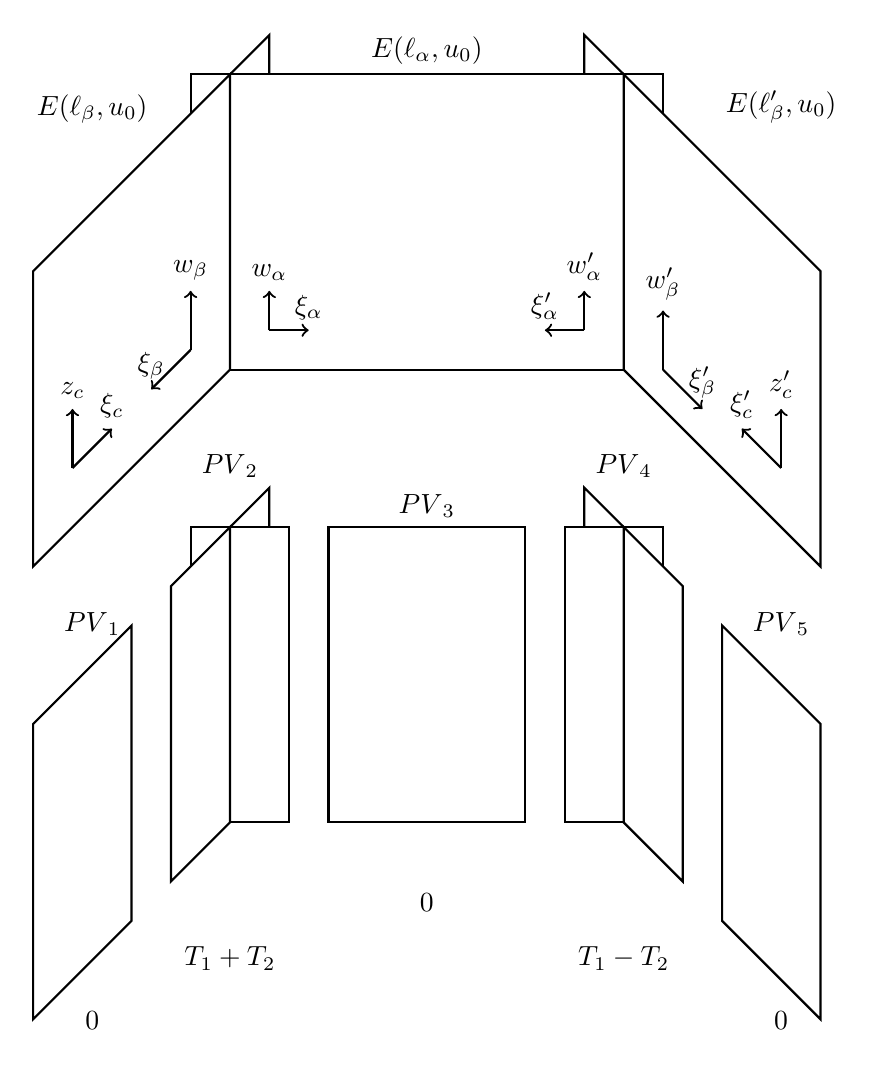
\begin{tikzpicture}[scale=2.5]
\draw[thick] (1,2.5) -- ++(0.2,0.2) -- ++(0,-0.2);
\draw[thick] (1,2.5)--(0.8,2.5)--(0.8,2.5-0.2);
\draw[thick] (0,0)--(1,1)--(1,2.5)--(0,1.5)--cycle;
\draw[thick](1,1)--(3,1) -- ++(0,1.5)-- ++(-2,0) -- cycle;
\draw[thick](3,1)--(4,0)-- ++(0,1.5)-- ++ (-1,1) --cycle;
\draw[thick](3,2.5) -- ++(0.2,0) -- ++(0,-0.2);
\draw[thick](3,2.5) -- ++(-0.2,0.2) -- ++(0,-0.2);
\draw (0.3,0.5+1.5+0.2) node[above] {$E(\ell_\beta,u_0)$};
\draw (2,2.5) node[above] {$E(\ell_\alpha,u_0)$};
\draw (3.8,0.5+1.5+0.2) node[above] {$E(\ell'_\beta,u_0)$};
\draw[thick,->] (0+0.2,0+0.5)--(0.2+0.2,0.5+0.2) node[above] {$\xi_c$};
\draw[thick,->] (0+0.2,0+0.5)-- ++ (0,0.3) node[right,above] {$z_c$};
%
\draw[thick,->] (1-0.2,1+0.1)-- ++ (-0.2,-0.2) node[left,above] {$\xi_\beta$};
\draw[thick,->] (1-0.2,1+0.1)-- ++ (0,0.3) node[left,above] {$w_\beta$};
%
\draw[thick,->] (1+0.2,1+0.2)-- ++ (0.2,0) node[left,above] {$\xi_\alpha$};
\draw[thick,->] (1+0.2,1+0.2)-- ++ (0,0.2) node[left,above] {$w_\alpha$};
%
\draw[thick,->] (3-0.2,1+0.2)-- ++ (-0.2,0) node[left,above] {$\xi'_\alpha$};
\draw[thick,->] (3-0.2,1+0.2)-- ++ (0,0.2) node[left,above] {$w'_\alpha$};
%
\draw[thick,->] (3+0.2,1)-- ++ (0.2,-0.2) node[right,above] {$\xi'_\beta$};
\draw[thick,->] (3+0.2,1)-- ++ (0,0.3) node[right,above] {$w'_\beta$};
%
\draw[thick,->] (4-0.2,0.5)-- ++ (-0.2,0.2) node[right,above] {$\xi'_c$};
\draw[thick,->] (4-0.2,0.5)-- ++ (0,0.3) node[right,above] {$z'_c$};
% PART II
% left bumps
\draw[yshift=-2.3cm,thick] (1,2.5) -- ++(0.2,0.2) -- ++(0,-0.2);
\draw[yshift=-2.3cm,thick] (1,2.5)--(0.8,2.5)--(0.8,2.5-0.2);
% left
%\draw[yshift=-2.3cm,thick] (0,0)--(1,1)--(1,2.5)--(0,1.5)--cycle;
\draw[yshift=-2.3cm,thick] (0,0)-- ++ (0.5,0.5) -- ++(0,1.5) -- ++(-0.5,-0.5)--cycle;
\draw[yshift=-2.3cm,thick] (0.7,0.7)--(1,1)-- ++(0,1.5) -- ++(-0.3,-0.3)--cycle;
% center
%\draw[yshift=-2.3cm,thick](1,1)--(3,1) -- ++(0,1.5)-- ++(-2,0) -- cycle;
\draw[yshift=-2.3cm,thick](1,1)-- ++(0.3,0) -- ++(0,1.5) -- ++(-0.3,0) --cycle;
\draw[yshift=-2.3cm,thick](1+0.5,1)-- ++(1,0) -- ++(0,1.5) -- ++(-1,0) -- cycle;
\draw[yshift=-2.3cm,thick](2.7,1)-- ++(0.3,0) -- ++(0,1.5) -- ++(-0.3,0) --cycle;

% right
%\draw[yshift=-2.3cm,thick](3,1)--(4,0)-- ++(0,1.5)-- ++ (-1,1) --cycle;
\draw[yshift=-2.3cm,thick](3,1)-- ++(0.3,-0.3) -- ++(0,1.5) -- ++ (-0.3,0.3)--cycle;
\draw[yshift=-2.3cm,thick](3+0.5,1-0.5)-- ++(0.5,-0.5) -- ++(0,1.5) -- ++ (-0.5,0.5)--cycle;
% right bumps
\draw[yshift=-2.3cm,thick](3,2.5) -- ++(0.2,0) -- ++(0,-0.2);
\draw[yshift=-2.3cm,thick](3,2.5) -- ++(-0.2,0.2) -- ++(0,-0.2);
\draw[yshift=-2.3cm] (0.3,0.2+1.5+0.2) node[above] {$\text{PV}_1$};
\draw[yshift=-2.3cm] (1,2.5+0.2) node[above] {$\text{PV}_2$};
\draw[yshift=-2.3cm] (2,2.5) node[above] {$\text{PV}_3$};
\draw[yshift=-2.3cm] (3,2.5+0.2) node[above] {$\text{PV}_4$};
\draw[yshift=-2.3cm] (3.8,0.2+1.5+0.2) node[above] {$\text{PV}_5$};
\draw[yshift=-2.3cm] (0.3,0.2+1.5+0.2-2) node[above] {$0$};
\draw[yshift=-2.3cm] (1,2.5+0.2-2.5) node[above] {$T_1+T_2$};
\draw[yshift=-2.3cm] (2,2.5-2) node[above] {$0$};
\draw[yshift=-2.3cm] (3,2.5+0.2-2.5) node[above] {$T_1-T_2$};
\draw[yshift=-2.3cm] (3.8,0.2+1.5+0.2-2) node[above] {$0$};
\end{tikzpicture}
\caption{This diagram 
should help to clarify coordinates patches.  It also 
identifies how the principal value integral will be broken into five pieces by
truncating the integrals near the poles.}
\end{figure}


%XX \midspace {6.5in} 
\wasacaption{\noindent }

Truncate near  $E(\ell_\beta,u_0) \cap E(\ell_\alpha,u_0)$\ in\ $E(\ell_\beta,u_0)$\
(The $\ell_\alpha$-pole) by
$$
\left| {\frac{-2T_2w_\beta +1}{(T_1-T_2)w_\beta +1}} \xi_\beta \right| \ge
q^{-m} .
$$

\noindent By (5.29) ${\dsize \frac{-2T_2w_{\beta} +1}{(T_1-T_2)w_{\beta} +1}} \xi_\beta$\  is a
variable over  $F$.  Since by (5.30)
$$
{\frac{1}{\xi_c+(T_1+T_2)z_c}} =  - {\frac{(-2T_2w_\beta +1)\xi_\beta}
{(T_1-T_2)w_\beta +1}}.
$$							    

%\pagebreak
\noindent
this region is the same as  $|\xi_c + (T_1 + T_2)z_c| \le q^{m}$.  Let
$\overline{\xi}_c = \xi_c + (T_1 + T_2)z_c$.  Then $z_c$  and  $\overline{\xi}_c$
are variables over $F$ and
$$
PV_1 = \int_{|\overline{\xi}_c|\le q^{m}} {d\overline{\xi}_c} 
\int_{\bold P^1} {\frac{dz_c}{|z_c^2|}}
= 0.
$$


\noindent  Truncate in  $E(\ell'_\beta, u_0)$\ near the $\ell'_\alpha$-pole by
$\dsize{\left| {\frac{-2T_2w'_\beta +1}{(T_1-T_2)w'_\beta +1}} \xi'_\beta \right|}
\ge q^{-m}$.  Then similarly\ $PV_5 = 0$.


\noindent  Truncate near the $\ell_\beta$-pole in\ $E(\ell_\alpha,u_0)$\ by
$|(2T_1w_\alpha +1)\xi_\alpha| \ge q^{-m}$\  and near the $\ell'_\beta$-pole
in\ $E(\ell_\alpha, u_0)$\  by\  $\dsize{\left| {\frac{(2(T_1-T_2)w_\alpha +1)}
{(-2T_2 w'_\alpha +1)}} \xi'_\alpha \right|} \ge q^{-m}$.\  $(2T_1w_\alpha +1)\xi_\alpha$\
and\  ${\dsize\frac{(2(T_1-T_2)w'_\alpha +1)}{(-2T_2w'_\alpha +1)}} \xi'_\alpha$\  are
variables over $F$.  Then since\ ${\dsize\frac{1}{(2T_1w_\alpha +1)\xi_\alpha}} =
{\dsize\frac{(-2(T_1-T_2)w'_\alpha + 1)}{(-2T_2w'_\alpha +1)}} \xi'_\alpha$\  let\ $\overline{\xi}_\alpha =
(2T_1w_\alpha +1)\xi_\alpha$.
$$
PV_3\ =\  \int_{q^{-m}\le |\overline{\xi}_\alpha|\le q^m}  
{\frac{d\overline{\xi}_\alpha}{|\overline{\xi}_\alpha|}}  \int_{{\bold P}^1}
{\frac{dw_\alpha}{|w_\alpha|^2}}\ = 0.
$$
	    

The contribution  $PV_4$  to the germ at the pole\ $\ell'_\beta \cap \ell_\alpha$\
is given by (1.3).  The function $M$ is given by $m(\alpha_0) + 2m$\ where $\alpha_0$
is defined by: 
$$
\alpha_0 = \lim_{\lambda\to 0}  
{\dsize\frac{\lambda}{\overline{\xi}'_\beta\overline{\xi}'_\alpha}} = 
\lim \left\{  \frac  {    { \dsize\frac{x(\alpha)x(\beta)w(\gamma)}{x(\gamma)} }           
                      } 
                     {    \left[ {\dsize \frac{2(T_1-T_2)w'_\alpha+1 }{ -2T_2w'_\alpha+1    } } \right]
                          \left[ {\dsize \frac{-2T_2w'_\beta+1       }{  (T_1-T_2)w'_\beta+1} } \right] 
                          \xi'_\alpha\xi'_\beta
                      }
     \right\}  
.
$$
\bigskip
	    

\noindent Here $\overline{\xi}'_\alpha$ and $\overline{\xi}'_\beta$\ are variables
over $F$.  Their definitions -- if not clear -- may be read off from the denominator
of this limit.
On\ $E_\alpha(u_0)$\ \ $x(\gamma)/x(\beta) = 1/2\xi'_\alpha$\ \ (5.8), on\ 
$E(\ell'_\beta,u_0)$\ $x(\gamma)/x(\alpha) = 1/\xi'_\beta$\ (5.27) and\
$w'_\alpha = w'_\beta = w(\gamma)$\ on their intersection so that
$$
\alpha_0 = \lim_{\lambda\to 0}\ {\dsize\frac{2x(\gamma)w(\gamma)((T_1-T_2)w(\gamma)+1)}
{(2(T_1-T_2)w(\gamma)+1)}}\ =\ {\dsize\frac{2x(\gamma)w_3}{(1-(T_1-T_2)^2w_3^2)}}
$$
\noindent where\ $w_3 = w'_\alpha/((T_1-T_2)w'_\alpha+1)$\  is a coordinate
over  $F$.  Thus  $M$  and hence $PV_4$  depend only on  $T_1-T_2$.

Similarly the factor $\alpha$  at the $(\ell_\beta \cap \ell_\alpha)$-pole is up to inessential
factors is
$$
{\dsize\frac{w}{({\dsize\frac{-2T_2w+1}{(T_1-T_2)w+1}})({\dsize\frac{2T_1w+1}{-2T_2w+1}})}}\ 
=\ {\frac{w_4}{(1-(T_1+T_2)^2w_4^2)}}
$$

\noindent where\ $w_4 = {\dsize\frac{w}{(T_1-T_2)w+1}}$\  is a variable over  $F$,
so that   $PV_2$  depends only on  $T_1+T_2$.
As in the proof of (5.23) we see that $PV_2$ is expressed in terms of the
corresponding terms $PV_2$ associated to a Cartan subgroup $T'$ contained
in a parabolic subgroup ($W_{T'} = \langle\sigma_\alpha\rangle$ or $\{1\}$)
for which compatibility is known.  The term $PV_4$ is analyzed similarly.
Hence the proposition follows.\end{proof}

%6
\section{The transfer of 2-regular germs of  GSp(4)}

\vskip .2in

There are no 2-regular elements in G(F) if G is not split.  Consequently, we
assume in this section that G is split.  We also take G = Sp(4) but since we
only prove the transfer of germs (2.8) for GSp(4) we assume that the 
endoscopic groups of G are cuspidal and split.  This leaves the group
H = SO(4).  We may make this assumption by the remark of (2.5) and the fact
that all the endoscopic groups of GSp(4) are split.  (They are split because
the derived group of the dual of GSp(4) is simply connected.)


Recall that all unipotent 2-regular elements are conjugate by $PSp(4,F)$\
or equivalently by\ $GSp(4,F)$.\  We have seen that there is one divisor
$E_2$  of the Igusa data which contributes to the 2-regular germ.  On the patch
$Y_U$,  $E_2$  is described by the equation\ $z(\alpha) = x(\alpha) =
x(\beta) = x(\gamma) = 0$.\ On the smaller patch where\ $x(\delta), w(\gamma) \ne 0$\
the equations become 
\begin{align*}
\lambda &= x(\gamma)^2 w(\delta)z(\beta)/(w(\gamma)^2x(\delta)) \tag {6.1}\\
x(\alpha) &= z(\beta)x(\gamma)/w(\gamma) \\
x(\beta) &= x(\gamma)^2 w(\delta)/(w(\gamma)^2 x(\delta)) \\ \vspace{1.5\jot}
z(\alpha) &= {\frac{x(\gamma)w(\delta)}{w(\gamma)x(\delta)}}
\end{align*}

\noindent and $E_2$  is described simply by\ $x(\gamma) = 0$.  Coordinates on
$E_2$  on this patch are\ $x(\delta)$, $w(\gamma)$, $w(\delta)$, $z(\beta)$, 
$v(\alpha)$, $v(\beta)$, $v(\gamma)$, $v(\delta)$.

By [Sp, p. 148]~~ ${\mathcal B}_{u_0}$\  the 2-dimensional variety of Borel
subgroups containing a given 2-regular element  $u_0$, contains a unique
projective line  $\ell_\beta$  of type $\beta$  and  ${\mathcal B}_{u_0}$\ is a
union of lines of type  $\alpha$  which intersect the line of type  $\beta$.
We consider the variety\ $E_2(u_0)$\ of all points $p$ of  $E_2$  above
$u_0 = \pi(p)\in G$.\  We fix a Borel subgroup  $B_0$  in the line  $\ell_\beta$
(whose points are Borel subgroups) and select any $B_\infty$  opposite  $B_0$.
Then by the choice of  $B_0$  $x_\alpha(u_0) = x_\beta(u_0) = x_\gamma(u_0) = 0$.\
Also if in the notation of (3.12) 
we have\ $(u, B_0^{n_W})^v \in E_2(u_0)$,\ then $x_\alpha(u) = x_\beta(u) =
x_\gamma(u) = 0$\  and  $u^v = u_0$.\  This forces\  $v = \exp(\xi x_{-\beta})$\
for some  $\xi$.  It follows that\ $x(\delta), v(\alpha), v(\gamma), v(\delta)$\
serve as coordinates on an open set of the conjugacy class\ $O_{u_0}$\ of
$u_0$  while\ $z\ {\mathrel{\mathop=^{def}}}\ z(\beta)$, 
$\xi\ {\mathrel{\mathop=^{def}}}\ v(\beta)$,\  
$w\ {\mathrel{\mathop=^{def}}}\ w(\gamma)$\  and
$\tilde{w}\ {\mathrel{\mathop=^{def}}}\ w(\delta)$\  serve as coordinates on an open
set of the fibre\ $E_2(u_0)$.\ We also set

\begin{align*}
w_A &= 2(T_1-T_2)w+1, \quad w_B = -2T_2w+1, \quad w_D = 2T_1w+1 \tag {6.2}\\
\ell &= \tilde{w}/w_B 
\end{align*}

The differential form on $E_2$  is\
$\omega_{E_2}\ {\mathrel{\mathop=^{def}}}\ 
Residue_{E_2}(\omega_Y/\lambda^\beta) \quad
\beta = b(E_2)/a(E_2) = 3$.
Using the coordinates of (6.1) we obtain
$$
\omega_Y/\lambda^3 = - x(\delta) {\frac{dz}{z^2}} {\frac{d\tilde{w}}{\tilde{w}^2}} dw
{\frac{dx(\gamma)}{x(\gamma)}} dx(\delta) d\xi dv(\alpha) dv(\gamma) dv(\delta)
$$
and
\begin{equation}
\omega_{E_2} = -x(\delta) {\frac{dz}{z^2}} {\frac{d\tilde{w}}{\tilde{w}^2}} dw\ dx(\delta)\
d\xi\ dv(\alpha)\ dv(\gamma)\ dv(\delta) . \tag {6.3}
\end{equation}

\noindent We separate this form into two parts:  an invariant form on the
conjugacy class\ $O_{u_0}$\  and a form on the fibre\ $E_2(u_0)$.\  
$\omega_0 = -x(\delta)dx(\delta)dv(\alpha) dv(\gamma) dv(\delta)$\  is easily
seen to be an invariant form on  $O_{u_0}$\ and  $\omega_{E_2(u_0)} =
{\dsize\frac{dz}{z^2}}\ {\dsize\frac{d\tilde{w}}{\tilde{w}^2}} dw d\xi$\  is then the form on the fibre
$E_2(u_0)$.

%\medpagebreak

Next we consider the action of the group $W\times A$  on the variables.  By our
choice of Borel subgroup  $B_0$, as with the subregular germs $A$ has two elements
$\{ 1,\sigma_0\}$.

Equations (5.10)  give the first two rows of (6.4)

\noindent (6.4)
$$
\begin{matrix} % \format \c &\quad \c &\quad \c &\quad \c &\quad \c &\quad \c &\quad \c \\
& \underline{w} & \underline{\ell} & \underline{z} & \underline{\xi} &
\underline{T_1} & \underline{T_2} \\
\vspace{2\jot}
\sigma_\alpha & \overline{w}/\overline{w}_A & \ell/(1+f_T\ell) & z/\overline{w}_A &
\xi & T_2 & T_1 \\
\vspace{1.5\jot}
\sigma\beta & w/w_B & \ell & z & 2T_2z+\xi & T_1 & -T_2 \\
\vspace{1.5\jot}
\sigma_0 & {(\xi w+z)/(\xi +2T_2z)} & \ell & {z/(\xi(2T_2z+\xi))}
& -1/\xi & T_1 & T_2
\end{matrix}
$$

\vskip .2in

\noindent We have used the abbreviations\ $\ell = \tilde{w}/w_B$, $\overline{w} = w + (T_1-T_2)\tilde{w}$,
$\overline{w}_A = w_A + (T_1-T_2)^2\tilde{w}$.  
The cocycle\ $t_\sigma$\  is given by\  $\sigma_\alpha\ \mapsto\ (1/x(\alpha))^{\alpha^v}$,\
$\sigma_\beta\ \mapsto\ (1/x(\beta))^{\beta^v}$,\ $\sigma_0 = A_\beta\
\mapsto\ (\xi_\beta)^{\beta^v}$.  
We adjust  $t_\sigma$  by  $c_\sigma = \sigma(t)t^{-1},  \quad t = (1, x(\alpha_1))$
\vskip .1in

\noindent $c_\sigma: \qquad \sigma_\alpha\ \mapsto\ (x(\alpha))^{\alpha^v}$,\ 
$\sigma_\beta\ \mapsto\ (w_Bx(\alpha)^2)^{-\beta^v}$,\ $\sigma_0\ \mapsto\ 
\xi_\beta^{-\beta^v}$
\vskip .1in

\noindent $c_\sigma t_\sigma:\quad  \sigma_\alpha\ \mapsto\ 1$,\ $\sigma_\beta\ \mapsto\
(w_Bx(\alpha)^2x(\beta))^{-\beta^v}$,\ $\sigma_0\ \mapsto\ 1$.
\vskip .1in

\noindent $\kappa$ is trivial on\ $d_\sigma$:\quad  $\sigma_\alpha\ \mapsto\ 1$,\
$\sigma_\beta\ \mapsto\ (\lambda^2)^{\beta^v}$,\ $\sigma_0\ \mapsto\ 1$.  So we may consider
\begin{equation}
c_\sigma t_\sigma d_\sigma\ =\ \sigma_\alpha\ \mapsto\ 1,\quad
\sigma_0\ \mapsto\ 1,\quad  \sigma_\beta\ \mapsto\ ({{z(\alpha)^2}\over {w_Bx(\beta)}} )^{\beta^v}
=\ \ell^{\beta^v}.  \tag {6.5}
\end{equation}
\vskip .1in

\noindent $\kappa(t_\sigma)\ =\ \kappa(t_\sigma'')$\  depends only on
$\ell$.


We recall the fact that\ $a(E_2)\ =\ 2$\  implies that there is a term of the
asymptotic expansion\ $F_1(\theta, 3)$\  for every character $\theta$ in  $F^\times$\
of order 2.		    

%\pagebreak
\proclaim{Proposition 6.6}~~ $F_1(\theta,3) = 0$\  if  $\theta$  is non-trivial.
\endproclaim

\begin{proof}  Let  $T_0$  be a split Cartan subgroup.  Then the action of  $G$ on
$Y_\Gamma$  gives an action of\ $T_0\subseteq\ G$\  on  $Y_\Gamma$.  To make this
explicit select two Borel subgroups\ $B_0,B_\infty$\  over  $F$  with\
$B_0 \cap B_\infty = T_0$.\  Then the action of\  $t_0\in T_0(\overline{F})$\  is
given on  $Y_1(B_\infty,B_0,\Sigma)$\  by
$$
(b, B_0^{n_W})^v\ \to\ (b, B_0^{n_W})^{v t_0} .
$$

\noindent In particular it acts on the fibres\ $\varphi^{-1}(\lambda)$\ in $Y_\Gamma$.\
Supposing\ $t_0\in C_G(u_0)(\overline{F})$,\ it is not difficult to see that the action on points\
$E_2(u_0)$\  above\ $u_0\in G(F)$\ in $E_2$ is given by
$$
z\ \longmapsto\ sz 
$$
$$
\xi\ \longmapsto\ s\xi
$$
$$
w\ \longmapsto\ w
$$
$$
\ell\ \longmapsto\ \ell
$$

\noindent  where\ $s = \beta(t_0)$.\  By (6.4) this morphism from\ $E_2(u_0)$\ to\
$E_2(u_0)$\  is defined over  $F$  provided\ $s\in F^\times$.\ Call this morphism
$\varphi_s$.

The morphism $\varphi_s$\ is easily seen to carry the form
$$
\omega_{E_2(u_0)}\ =\ {dz\over z^2}~ {d\tilde{w}\over \tilde{w}^2}~ dw~d\xi \quad {\text{to itself}}.
$$


\noindent  The action of  $\varphi_s$  on  $m_{\theta,E}$\  is also easily calculated.
By (6.4)\ $\sigma(x(\gamma))x(\gamma)^{-1}$\  for\ $\sigma\in Gal(\overline{F}/F)$\
evaluated on  $E_2$  is a function of\ $w,\ell$\  and the tangent direction of
$\Gamma$  but not of $\xi$  or  $z$.  By Hilbert's 90th we write\
${\widetilde{x(\gamma)}} = x(\gamma)a$\  with\ $a$ a function of\ $w, \ell$\ and
the  tangent direction, and $\widetilde{x(\gamma)}$ a variable over F.  Then
$$
\lambda\ =\ {{x(\gamma)^2\tilde{w}z}\over {w^2x(\delta)}}\ 
=\ {{{\widetilde{x(\gamma)}}^2\tilde{w}z}\over
{a^2w^2x(\delta)}}		 
$$

\noindent  and $\theta(\lambda)\ =\ \theta({{\tilde{w}z}\over {a^2w^2x(\delta)}})$.\  Thus
$$
m_{\theta,E}\ {\mathrel{\mathop=^{def}}}  \lim_{\lambda\to 0}\ {{\kappa(t_\sigma)}\over
{\theta(\lambda)}}\ =\ {{\kappa(t_\sigma)}\over {\theta({{\tilde{w}z}\over {a^2w^2x(\delta)}})}}.
$$

\noindent  $t_\sigma$  depends only on $\ell$  so that  $\varphi_s$\ carries
$m_{\theta,E}$\ to\
$$
{{\kappa(t_\sigma)}\over {\theta({{\tilde{w}\ z\ s}\over{a^2w^2x(\delta)}})}}\ =\ {{m_{\theta,E}}\over
{\theta(s)}}.
$$

\noindent  A change of coordinates does not change a principal value integral.
Changing coordinates on\ $E_2(u_0)$\ by the automorphism\ $\varphi_s$\  gives

$$
F_1(\theta,3) = \left[ \int_{E_2(u_0)} m_{\theta,E} |\omega_{E_2(u_0)}|\right] \mu^H_O(f)\
=\ {{1}\over {\theta(s)}} \left[ \int m_{\theta,E} |\omega_{E_2(u_0)}|\right]
\mu^H_O (f).
$$

\noindent  So that if  $\theta(s)\ne 1$\ for some\ $s\in F^\times$\  we must have\
$F_1(\theta,3)\ =\ 0$.\
\end{proof}

We turn to the Cartan subgroups associated to the endoscopic group  SO(4).  We define
a birational map from\ $E_2(u_0)$\ to\ $({\bold P}^1)^4$\  by
\begin{align*}
w_2 &= {{-T_1w_B+\ell_1}\over {T_2w_B}}  \\ \vspace{2\jot}
\ell_2 &= {{f_T\ell}\over {f_T\ell +2}} \\ \vspace{2\jot}
\xi_1 &= \xi  \\ \vspace{2\jot}
\xi_2 &= \xi + \rho z 	\end{align*}
\qquad 
\begin{align*}
\ell_1 & {\mathrel{\mathop=^{def}}}\ (1 + T_2(T_1+T_2)\ell)(T_1 +T_2)\\
\vspace{2\jot}
w_B & {\mathrel{\mathop=^{def}}}\ (-2T_2w+1) \\ \vspace{2\jot}
f_T & {\mathrel{\mathop=^{def}}}\ (T^2_2 - T^2_1) \\ \vspace{2\jot}
\rho & {\mathrel{\mathop=^{def}}}\ {{2T_2\ell_1}\over {-T_1w_B+\ell_1}}
\tag {6.7}
\end{align*}



\noindent  where\ $w_2, \ell_2, \xi_1, \xi_2$\  are coordinates on\ $({\bold A}^1)^4 \subseteq
({\bold P}^1)^4$.\  The map is birational, for it may be inverted by inverting the
relations for\ $\ell_2, \xi_1, w_2$\ and\ $\xi_2$\ in that order.  The form\
$\omega_{E_2(u_0)}$\  in these coordinates is found to be

\begin{equation}
{{(T^2_2-T^2_1)}\over {2}} ~ {{d\ell_2}\over {\ell_2^2}} ~ {{dw_2}\over {w_2}} ~
{{d\xi_1 d\xi_2}\over {(\xi_1-\xi_2)^2}}\ =\ \omega_{E_2(u_0)}  \tag {6.8}
\end{equation}


Transferring the action of\ $W\times A$\  via (6.7) to the coordinates\ $w_2, \ell_2,
\xi_1, \xi_2$\ gives:
\vskip .2in

\noindent (6.9)
$$
\begin{matrix} % \format \c & \quad \c &\quad \c &\quad \c &\quad \c \\
& \underline{1} & \underline{\sigma_\alpha} & 
\underline{\sigma_\beta\sigma_\alpha\sigma_\beta}
& \underline{\sigma_0} \\
\vspace{2\jot}
w_2 & w_2 & w_2/f^2 & 1/w_2 & (\xi_2/\xi_1)w_2 \\
\vspace{1.5\jot}
\ell_2 & \ell_2 & -\ell_2 & -\ell_2 & \ell_2 \\
\vspace{1.5\jot}
\xi_1 & \xi_1 & \xi_1 & \xi_2 & -1/\xi_1 \\
\vspace{1.5\jot}
\xi_2 & \xi_2 & \xi_2 & \xi_1 & -1/\xi_2
\end{matrix}
$$
\vskip .2in

\noindent  where\  $f = \left( {\dsize\frac{1+\ell_2}{1-\ell_2}}\right)$.

 
$t_\sigma''$  is given by\ $\sigma_0\ \to\ 1$,~ $\sigma_\alpha\ \to\ 1$,\ 
$\sigma_\beta\ \to\ \ell^{\beta^v}\ =\ ({\dsize\frac{2w}{f_T}}\ 
{\dsize\frac{1}{1-w}})^{\beta^v}$.\
The factor\ ${{2w}/{f_T}}$\  lies in  $F^\times$  so that  $\kappa(t_\sigma) =
\kappa(t'_\sigma)$\  where  $t'_\sigma$  is defined by\  $\sigma_0 \to 1, 
\sigma_\alpha \to 1$,\ $\sigma_\beta \to (1-w)^{-\beta^v}$.\  This implies that
$\sigma_\beta\sigma_\alpha\sigma_\beta\ \to\ ((1+w)^{-1}, (1-w)^{-1}, 1-w, 1+w)$\ 
so that as in the proof of (5.2.3) $\kappa(t_\sigma) = \eta_{E'}(1-w^2)$\ where\ 
$E' = Inv(\sigma_0,\sigma_\alpha)$\ 
the field invariant by $\sigma_\alpha$ and $\sigma_0$.

We may always choose the homomorphism\ Gal$(\overline{F}/F)\ \to A$\  so that\
$\xi_1, \xi_2 = 0,\infty$\  are not rational points.  Thus\ $\xi_2/\xi_1 \ne 0,\infty$\
and is well defined.  Assume that such a choice is made.  Also if\ 
Im((Gal$(\overline{F}/F) \subseteq W)\ =\ \langle \sigma_\alpha \sigma_\beta
\sigma_\alpha \sigma_\beta\rangle$\ then\ $\ell_2 = \pm 1$, $f = 0,\infty$\  are $F$-rational
points so that the action of\ $\sigma_\alpha \sigma_\beta \sigma_\alpha \sigma_\beta$
on $w_2$ for\ $f = 0,\infty$\ is not defined.  But this has an effect 
because the integrals are principal value integrals.

The following lemma is proved in section   7.

\proclaim{Lemma 6.10}  The principal value integral\ 
$\int_{E_2(u_0)} m_{\kappa,E}\,|\omega_{E_2}(u_0)|$\
is preserved under the birational map (6.7).
\endproclaim

\proclaim{Corollary\ \ 1}  The 2-regular germ is zero if  $\kappa$ is trivial and
$W_T \subseteq \langle 1, \sigma_\alpha, \sigma_\beta\sigma_\alpha\sigma_\beta\rangle$.
\endproclaim

\begin{proof}  For  $s\in F^\times$  the automorphism of  $E_2(u_0)$\ sending
$w_2$ to $w_2$,  $\ell_2$ to $s\ell_2$, $\xi_1$ to $\xi_1$ and $\xi_2$ to $\xi_2$  is  defined
over $F$.  It takes the form\ $\omega_{E_2(u_0)}$  
to\ $\omega_{E_2(u_0)}/{s}$\ so that changing coordinates using this automorphism 
$$
\int_{E_2(u_0)} |\omega_{E_2(u_0)}|\ =\ {{1}\over {|s|}} \int_{E_2(u_0)}
|\omega_{E_2(u_0)}| (= 0 \quad {\text{if}} ~~ |s| \ne 1).
$$
\end{proof}

\proclaim{Corollary\  2}  The 2-regular germs have the form\ 
$|T_1^2-T^2_2| c(T,\kappa)$\  for some constants\ $c(T,\kappa)$\ depending on  $(T,\kappa)$.
\endproclaim

\begin{proof}  The data (6.9) is independent of  $T_1,T_2$ and\
$|\omega_{E_2(u_0)}| = |T_1^2-T^2_2|$\ $|\omega'|$\ where $\omega'$  is a form independent
of  $T_1,T_2$.
\end{proof}


\proclaim{Corollary\  3}  The transfer of orbital integrals in (2.8) holds for a
function  $f^H$  independent of  $(T,\kappa)$\ associated to\ $H = SO(4)$.
\endproclaim

\begin{proof}  To prove the compatiblity of functions  $f^H$  for various choices
of  $(T,\kappa)$\ associated to $SO(4)$  we reason as follows.  We write 
$T/(\pm 1) = S_1\times S_2$\ where the tangent direction in  $S_1$  is  $T_1-T_2$\
and $T_1+T_2$\ in $S_2$.  Fix a function  $f\in C_c^\infty(G)$\ such that
$\mu_0^H(f) = 0$\ if  $O$  is not 2-regular.  Using transfer factors\
$\Delta_H^{T,\kappa}$\ we fix normalized subregular germs\ $A_{S_1}, B_{S_2}$\ on
$H$.\ $A_{S_1}$\ are functions on  $S_1$ of the form\ $\lambda|T_1-T_2|a_{S_1}$,\
$a_{S_1}$\ a constant independent of  $S_2$ (see [LS]).  Similarly\
$B_{S_2} = \lambda|T_1+T_2|b_{S_2}$.\ By (2.9)\ 
$$\Delta_G^{T,\kappa}\Phi_G^{T,\kappa}
= \lambda^2|T_1^2-T_2^2|c(T,\kappa) = \lambda|T_1-T_2|a_{S_1} 
\mu_{O'}^{H'}(f_{qs}).$$
\noindent It was argued in (2.9) that  $f_{qs}$  is independent of  $T_1-T_2$.
The choice of  $f_{qs}$  may also
be made independently of  $S_1$.  To see this  we use the explicit formula for
$f^M$ in [R] and note that the choice of  $f_{qs}$  in the definition of  QSR\
$(2.10)$\ may be chosen independently of  $S_1$.  Thus we conclude 

%\pagebreak
that\
$\mu_0^{H'}(f'_{qs}) = |T_1+T_2|b'_{S_2}$\ or\ $c(T,\kappa) = a_{S_1}b'_{S_2}$\
for some constants  $b'_{S_2}$.\ Reversing the roles of  $S_1$  and $S_2$  we have
$c(T,\kappa) = a'_{S_1}b_{S_2}$\  for constants  $a'_{S_1}$.\  We conclude that
$c(T,\kappa) = \alpha_1 a_{S_1}b_{S_2}$\ for some constant $\alpha_1$.  Thus the
2-regular germ is\ $\alpha_1\lambda^2|T_1^2-T_2^2|a_{S_1}b_{S_2} = 
\alpha_1 A_{S_1} B_{S_2}$\  which up to scalar $\alpha_1$ is the 2-regular germ
on $H$.
\end{proof}

%7
\section{Spurious Divisors and some technical details}


This final section contains the remaining details of the proof of the transfer
of orbital integrals on  GSp(4).  It is shown that the construction in the preceding
sections satisfies the conditions of (1.1), none of the divisors outside of  $Y_U$  
contributes to the germ expansion, any amount of blowing up along subvarieties
of divisors outside of $Y_U$ has no effect on the subregular germs, and the
birational map\ $E_2(u_0)\ \to\ ({\bold P}^1)^4$\  of (6.7) preserves 
principal value integrals.

To obtain coordinates outside $Y_U$ we construct the variety $Y_\Gamma$  from
scratch.  The variety of stars is defined on an open patch\ $S(B_\infty, B_0)$\
by 
\begin{equation}
\epsilon_{-\alpha}(s_4)\epsilon_{-\beta}(r_4)\epsilon_{-\alpha}(s_3)\epsilon_{-\beta}(r_3)
\epsilon_{-\alpha}(s_2)\epsilon_{-\beta}(r_2)\epsilon_{-\alpha}(s_1)\epsilon_{-\beta}(r_1)\
=\ 1. \tag {7.1}
\end{equation}

\noindent where\ $\epsilon_{-\alpha}(s) = {\begin{pmatrix} 1&&&\\ s&1&&\\ &&1&\\ 
&&-s&1 \end{pmatrix}}$\  and\  $\epsilon_{-\beta}(r)\ =\ 
{\begin{pmatrix} 1&&&\\ &1&&\\ &r&1&\\ &&&1 \end{pmatrix}}$.
\vskip .2in

Multiplying out the relation (7.1) we obtain

\noindent %flushpar
(7.2)
$$\begin{matrix} % \format \l & \c \\
\vspace{1\jot}
s_1+s_2+s_3+s_4 = 0 & \\
\vspace{1\jot}
r_1+r_2+r_3+r_4 = 0 & \\
\vspace{1\jot}
r_2s_1+r_3(s_1+s_2)+r_4(s_1+s_2+s_3) = 0 & \\
\vspace{1\jot}
r_2s_2^2 + r_3(s_1+s_2)^2+r_4(s_1+s_2+s_3)^2 = 0 & \end{matrix}
$$
\vskip .2in
\noindent %flushpar

There is a\ ${\bold G}_m\times {\bold G}_m$\  action on\ $S(B_\infty, B_0)$\ given
by\ $(s_i,r_i)\ \mapsto\ (ss_i,rr_i)$.\   There is an action of the cyclic group of
order four given by \ $(s_i,r_i)\ \mapsto\ (s_{i+1},r_{i+1})$\  with indices read
modulo 4 and an action of an involution given by\ $(s_i,r_i)\ \mapsto\ 
(-s_{1-i}, -r_{2-i})$.\  They combine to give an action of the Weyl group on\
$S(B_\infty, B_0)$\  which commutes with the\ ${\bold G}_m \times {\bold G}_m$
action.

We note for future reference that the equation (7.2) imply

\noindent %flushpar
(7.3) \qquad \qquad  $r_2s_1s_2 = -r_4s_4s_3$\ plus identities obtained by permuting
the indices cyclically.

There is a proper morphism\ $S_1\ {\dsize\mathrel{\mathop\rightarrow^{\varphi}}}\ S$\
where\  $S_1(B_\infty,B_0) = \varphi^{-1}S(B_\infty, B_0)$\  is covered by 
coordinate patches\ $U(m,n) \quad  m,n\in \{ 1,2,3,4\}$.    The coordinates and
relations on\ $U(m,n)$\ are

%\pagebreak
\noindent %flushpar

(7.4)
$$\begin{matrix} % \format \l & \c \\ 
r,s, R_1, R_2, R_3, R_4, S_1, S_2, S_3, S_4 
{\text{\qquad satisfying~the~ relations}}& \\
\vspace{1.5\jot}
R_m = S_n = 1 & \\
\vspace{1\jot}
S_1 + S_2 + S_3 + S_4 = 0 & \\
\vspace{1\jot}
R_1 + R_2 + R_3 + R_4 = 0 & \\
\vspace{1\jot}
R_2S_1 + R_3(S_1 + S_2) + R_4(S_1 + S_2 + S_3) = 0 \\
\vspace{1\jot}
R_2 S_1^2 + R_3(S_1 + S_2)^2 + R_4(S_1 + S_2 + S_3)^2 = 0
\end{matrix}
$$
\vskip .2in
\noindent %flushpar

The morphism\ $\varphi $\ from  $U(m,n)$  to  $S(B_\infty, B_0)$\  is given by
$(S_i, R_j, s, r)\ \mapsto\ (sS_i, rR_j)$.  
It is proved in [H] that\ $\varphi $\ is a proper map from $S_1$ to $S$.

\proclaim{Lemma\ \ 7.5}  (a)  $S_1$  is covered by patches isomorphic to  $U(1,1)$
\noindent %flushpar
(b)  $S_1$  is nonsingular.
\endproclaim

\begin{proof}  (a)\ The patches\ $S(B_\infty, B_0)$ \ as  $(B_\infty, B_0)$\ vary 
are all isomorphic.  So we may fix\ $(B_\infty, B_0)$.
\end{proof}


Let $Z = \{R_1,R_2,R_3,R_4,S_1,S_2,S_3,S_4\}$\  and for\  $p\in U(m,n)$\ set
$Z_p = \{z\in Z \mid z(p) = 0\}$.\  The possibilities for $Z_p$  are calculated
in [H].  Up to a symmetry of the Weyl group acting on the indices they are

\begin{figure}[htb]
\centering
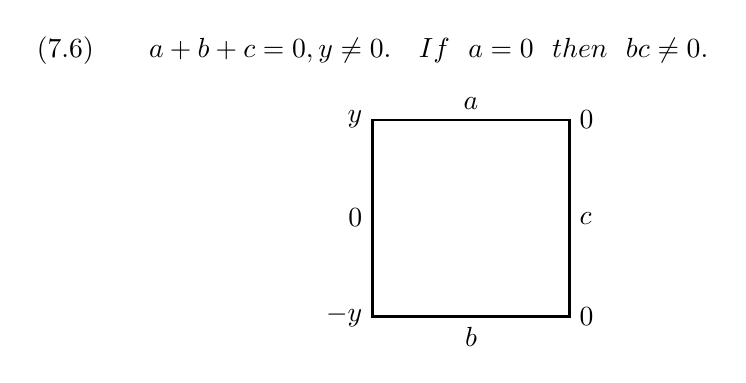
\begin{tikzpicture}[>=angle 90,scale=2.5]
\node[] at (0,0.35) {
{(7.6)}\qquad $a+b+c = 0, y\ne 0.\quad  {\text{If}}~~ a = 0~~{\text{then}}~~ bc\ne 0.$
};
\draw[thick]
(0,0) node[above,left]{$y$}
-- ++(0:0.5) node[above]{$a$}
-- ++(0:0.5) node[above,right]{$0$}
-- ++(270:0.5) node[right]{$c$}
-- ++(270:0.5) node[below,right]{$0$}
-- ++(180:0.5) node[below]{$b$}
-- ++(180:0.5) node[below,left]{$-y$}
-- ++(90:0.5) node[left]{$0$}
-- cycle;
\end{tikzpicture}
\end{figure}

%7.7
\begin{figure}[htb]
\centering
\begin{tikzpicture}[>=angle 90,scale=2.5]
\node[] at (0,0.35) {
{(7.7)}\qquad 
$a+b+c = 0 \quad x\ne 0. ~~~{\text{If}}~~ b = 0 ~~ {\text{then}}~~ac \ne 0.$
};
\draw[thick]
(0,0) node[above,left]{$a$}
-- ++(0:0.5) node[above]{$0$}
-- ++(0:0.5) node[above,right]{$c$}
-- ++(270:0.5) node[right]{$-x$}
-- ++(270:0.5) node[below,right]{$0$}
-- ++(180:0.5) node[below]{$x$}
-- ++(180:0.5) node[below,left]{$b$}
-- ++(90:0.5) node[left]{$0$}
-- cycle;
\end{tikzpicture}
\end{figure}

%7.8
\begin{figure}[htb]
\centering
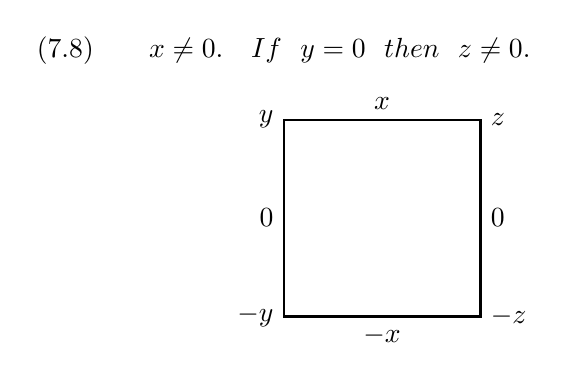
\begin{tikzpicture}[>=angle 90,scale=2.5]
\node[] at (0,0.35) {
{(7.8)}\qquad 
$x\ne 0.~~~{\text{If}}~~y = 0 ~~{\text{then}}~~ z\ne 0.$
};
\draw[thick]
(0,0) node[above,left]{$y$}
-- ++(0:0.5) node[above]{$x$}
-- ++(0:0.5) node[above,right]{$z$}
-- ++(270:0.5) node[right]{$0$}
-- ++(270:0.5) node[below,right]{$-z$}
-- ++(180:0.5) node[below]{$-x$}
-- ++(180:0.5) node[below,left]{$-y$}
-- ++(90:0.5) node[left]{$0$}
-- cycle;
\end{tikzpicture}
\end{figure}

%7.9
\begin{figure}[htb]
\centering
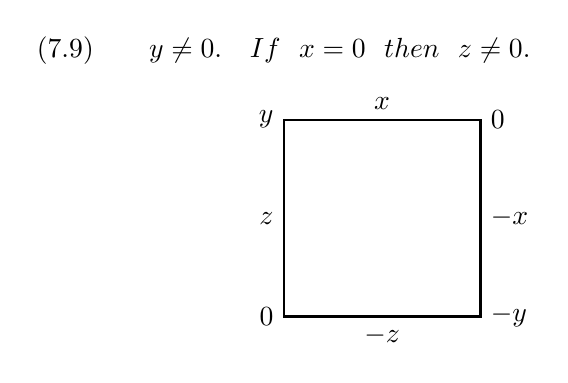
\begin{tikzpicture}[>=angle 90,scale=2.5]
\node[] at (0,0.35) {
{(7.9)}\qquad 
$y\ne 0.~~~{\text{If}}~~ x = 0~~{\text{then}}~~z\ne 0.$
};
\draw[thick]
(0,0) node[above,left]{$y$}
-- ++(0:0.5) node[above]{$x$}
-- ++(0:0.5) node[above,right]{$0$}
-- ++(270:0.5) node[right]{$-x$}
-- ++(270:0.5) node[below,right]{$-y$}
-- ++(180:0.5) node[below]{$-z$}
-- ++(180:0.5) node[below,left]{$0$}
-- ++(90:0.5) node[left]{$z$}
-- cycle;
\end{tikzpicture}
\end{figure}
\noindent %flushpar 

\begin{figure}[htb]
\centering
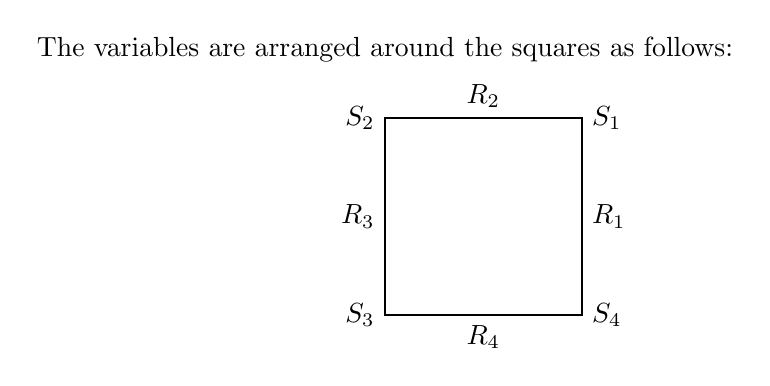
\begin{tikzpicture}[>=angle 90,scale=2.5]
\node[] at (0,0.35) {
The variables are arranged around the squares as follows:
};
\draw[thick]
(0,0) node[above,left]{$S_2$}
-- ++(0:0.5) node[above]{$R_2$}
-- ++(0:0.5) node[above,right]{$S_1$}
-- ++(270:0.5) node[right]{$R_1$}
-- ++(270:0.5) node[below,right]{$S_4$}
-- ++(180:0.5) node[below]{$R_4$}
-- ++(180:0.5) node[below,left]{$S_3$}
-- ++(90:0.5) node[left]{$R_3$}
-- cycle;
\end{tikzpicture}
\end{figure}



\hrule height0pt width6true in
\vskip 1.8 true in 

\noindent %flushpar
Notice that (7.3) now states that the product of variables along an edge is the
negative of the product of variables along the opposite edge.

\noindent %flushpar
By examining (7.6)-(7.9) it is evident that there are always two adjacent variables
on the square that are non-zero.  By the action of the Weyl group, we may take the
adjacent variables to be  $R_1, S_1$.  Such a point is contained in a patch
isomorphic to  $U(1,1)$.  This proves (a).

(b)\ By (a) it is enough to prove that  $U(1,1)$  is nonsingular.  We consider
two patches $A$ and $B$.

\noindent %flushpar
(A)\  Let  $x = S_4$,  $y = S_3R_4$.\  Then inverting the relations (7.2) we find
\noindent %flushpar
(7.10)
$$\begin{matrix} % \format \l &\qquad\l \\
S_1 = 1 & R_1 = 1 \\
S_2 = xy+y-1 & R_2 = -xy/(xy+y-1) \\
S_3 = -x-y-xy & R_3 = x/((xy+y+x)(xy+y-1)) \\
S_4 = x & R_4 = -y/(xy+y+x)
\end{matrix}
$$
\vskip .2in

\noindent %flushpar

We see that $x$ and $y$  are local coordinates, unless $(x,y) = (0,1)$ or
$(0,0)$.  (Unless the numerator and the denominator of  $R_2,R_3$, or  $R_4$  
simultaneously vanish, $x$ and $y$  describe a pont in  $S_1(B_\infty, B_0)$\
although not necessarily a point in\ $U(1,1)$).  By (7.10) it follows that

\begin{equation}
t{\mathrel{\mathop=^{def}}} y/x = {\frac{S_3R_4}{S_4}} = {\frac{-R_4}{S_2R_3}} =
{\frac{R_2}{R_3S_3S_4}} . \tag {7.11}
\end{equation}

\noindent %flushpar

Near  $(x,y) = (0,0)$  we may select coordinates  $(x,t)$ or  $(y,1/t)$\ unless
$R_2 = R_4 = S_4 = 0, \quad R_1 = S_1 = 1, \quad S_2R_3 = 0$.\ But the list of
possible patterns  $Z_p$  in (7.6)-(7.9)  shows that this never occurs.  We conclude
that patch (A) (together with the variants $(x,t)$ or $(y,1/t)$) 
covers points such that\ $(x,y)\ne (0,1)$,
i.e., \quad $S_4 = 0,
S_3R_4 = 1$.
\vskip .2in
\noindent %flushpar

(B)  Let  $S_1 = R_1 = 1,\ a = S_2,\ b = R_3$.\ Then inverting the relations
(7.4) we find

\noindent (7.12)
$$
\begin{matrix} % \format \l & \qquad \l \\
S_1 = 1 & R_1 = 1 \\
S_2 = a & R_2 = -b(1+a)^2/(1+ba^2) \\
S_3 = (1+a)/(ab-1) & R_3 = b \\
S_4 = -ab(1+a)/(ab-1) & R_4 = -(ab-1)^2/(1+ba^2) 
\end{matrix}
$$
\vskip .2in

\noindent %flushpar
We see $a$ and $b$  are local coordinates unless  $ab = 1$  and  $1+a = 0$, i.e.,\
$a = -1$, $b = -1$ \quad $(S_2 = -1, S_1 = 1, R_3 = -1)$.

\noindent %flushpar
Points in the complement of both patches must satisfy\ $R_1,S_1,S_2,R_3,S_3,R_4 
\ne 0$.  This is impossible by the list of possible patterns (7.6)-(7.9).

\noindent %flushpar
Next we turn to a calculation of\ $t^{-1}n^{-1}t\ n \in N$\  
for\ $n\in N, t\in T$.  Using the notation following (5.26) we let
\begin{align*}
n &= m(n_\beta, n_\alpha, n_\gamma, n_\delta) \qquad \qquad (n'_\gamma =\
n_\gamma - n_\alpha n_\beta) \\
y &= m(y_\beta, y_\alpha, y_\gamma, y_\delta) \qquad \qquad (y'_\gamma =\
y_\gamma - y_\alpha y_\beta), \qquad  n,y \in N  \\
t &= {\text{diag}}(t_1,t_2,t_2^{-1},t_1^{-1}) \in T.
\end{align*}
\vskip .2in

%\pagebreak
\proclaim{Lemma\ \ 7.13}  
\begin{align*}
y_\alpha &= (1-t_2t_1^{-1})n_\alpha \\
y_\beta &= (1-t_2^{-2})n_\beta \\
y_\gamma &= (1-t_2^{-1}t_1^{-1})n_\gamma + (t_2^{-1}t_1^{-1}-t_2t_1^{-1})n_\alpha n_\beta \\
y'_\gamma &= (1-t_2^{-1}t_1^{-1})n_\gamma + (t_2^{-2}-1)n_\alpha n_\beta \\
y_\delta &= (1-t_1^{-2})n_\delta + (t_2^{-1}t_1^{-1}-t_2t_1^{-1})n_\alpha n'_\gamma
\end{align*}
\vskip .1in

\noindent provided\ $y = t^{-1}n^{-1}t\ n$.
\endproclaim

\begin{proof}\ Elementary matrix computation.
\end{proof}

By definition (3.12)\ $w(\alpha) = w(\beta) = 1$, $w(\gamma) = \lambda y_\gamma /y_\alpha y_\beta$\
and\ $w(\delta) = \lambda^2y_\delta /y^2_\alpha y_\beta$\  so that with\
$\alpha = t_1t_2^{-1}, \beta = t_2^2, \gamma = t_1t_2, \delta = t_1^2$\ we have:

\noindent (7.14)
\begin{align*}
w(\gamma) &= {\frac{(1-\gamma^{-1})\lambda}{(1-\alpha^{-1})(1-\beta^{-1})}}\
\left( {\frac{n_\gamma}{n_\alpha n_\beta}} \right)  +  {\frac{(\gamma^{-1}-\alpha^{-1})\lambda}
{(1-\alpha^{-1})(1-\beta^{-1})}} \\
\vspace{2\jot}
w(\delta) &= {\frac{\lambda^2(1-\delta^{-1})}{(1-\alpha^{-1})^2(1-\beta^{-1})}}\
\left( {\frac{n_\delta}{n^2_\alpha n_\beta}} \right)  +
{\frac{\lambda^2(\gamma^{-1}-\alpha^{-1})}{(1-\alpha^{-1})^2(1-\beta^{-1})}}
\left( {\frac{n'_\gamma}{n_\alpha n_\beta}}\right).
\end{align*}
\noindent %flushpar
To complete the description of  $w(\gamma)$  and  $w(\delta)$\  it is necessary
to compute\ $n_\gamma/(n_\alpha n_\beta))$\ and\ 
$n_\delta/(n_\alpha^2n_\beta)$\ in terms of coordinates on the star
variety.  The functions\ $n_\alpha, n_\beta, n_\gamma$\ and\ $n_\delta$\  are 
determined by the relation\ ${\bold B}n_Wn^{-1} \in {\bold B}\omega$\  for all
$\omega \in W$\ (the Weyl group) with\ $W = W(\omega)$\ (a Weyl chamber).

\proclaim{Lemma\ \ 7.15}  $n'_\gamma/n_\alpha n_\beta = S_4/S_1$,\
$n_\gamma/(n_\alpha n_\beta) = (S_4/S_1) + 1$, 
$n_\delta/(n_\alpha^2n_\beta) = (R_1S_4)/(R_4S_3)$,\
$z(\alpha) = -s_4\lambda/(1-\alpha^{-1})$, $z(\beta) = 
r_1\lambda/(1-\beta^{-1})$.
\endproclaim

\begin{proof}  The final two relations are found in both [L] and [H].  By
$n_Wn^{-1} \in {\bold B}\omega$\ we have (by writing out these matrices)

%\pagebreak

$n_\alpha = -1/s_4, n_\beta = 1/r_1, n'_\gamma = -n_\beta/s_1 = -1/r_1s_1$.
$n_\gamma = n'_\gamma + n_\alpha n_\beta = -1/r_1s_1\ -1/r_1s_4,\ r_4s_4n_\delta =
n_\alpha + r_4n_\gamma = -1/s_4 - r_4/r_1s_1 -r_4/r_1s_4 = 
-(r_1s_1+s_4r_4+r_4s_1)/r_1s_1s_4 = -r_3s_2/(r_1s_1s_4) = 
-r_3s_2/(-s_2r_3s_3) = 1/s_3$,\ $n_\delta = 1/(s_3r_4s_4) =
-1/(r_2s_1s_2)$.  We have made use of (7.2) and (7.3).  
This completes the proof.
\end{proof}

Now combining (7.14) and (7.15) with\ $A = (1-\alpha^{-1})/\lambda, \quad
B = (1-\beta^{-1})/\lambda, \quad C = (1-\gamma^{-1})/\lambda, \quad
D = (1-\delta^{-1})/\lambda$\ we find

\noindent (7.16)
$$
\begin{matrix} %\format \l & \l \\
w(\gamma) &= {\dsize\frac{C}{AB}}({\dsize\frac{s_4}{s_1} + 1}) 
+ {\dsize\frac{(A-C)}{AB}} \\ \vspace{2\jot}
{} & = \qquad
{\dsize\frac{C}{AB}}{\dsize\frac{s_4}{s_1}}\ + {\dsize\frac{1}{B}}\\
\vspace{2.5\jot}
w(\gamma) &= {\dsize\frac{D}{A^2B}}\ {\dsize\frac{(r_1s_4)}{(r_4s_3)}} + 
{\dsize\frac{(A-C)}{(A^2B)}}
{\dsize\frac{s_4}{s_1}} \\
\vspace{2\jot}
{} &= \qquad {\dsize\frac{(s_4r_1)}{(r_4s_3)}} ) ({ 
{\dsize\frac{D}{A^2B}}{\dsize\frac{r_1s_1}{r_1s_1}} + 
{\dsize\frac{(A-C)}{A^2B}} {\dsize\frac{r_4s_3}{r_1s_1}} }).
\end{matrix}
$$
\vskip .2in

\noindent We are now in a position to identify all divisors and calculate their
associated constants\ $a(E)$, $b(E)$, $\beta(E)$.\  By (7.5) we may assume that\
$R_1 = S_1 = 1$.

Begin with the assumption that\ $g\ {\mathrel{\mathop=^{def}}}\ \left(
{\frac{D}{A^2B}} + {\frac{A-C}{A^2B}} R_4 S_3 \right) \ne 0$\ at $p$, a point on the
divisor $E$.  We consider several patches.  We begin by using (7.15), (7.16) to rewrite
the equations
\begin{align*}
\lambda w(\delta) &= z(\alpha)^2z(\beta)x(\delta) \\
x(\alpha) &= {\frac{\lambda}{z(\alpha)}} \\
x(\beta) &= {\frac{\lambda}{z(\beta)}} \\
x(\gamma) &= {\frac{\lambda w(\gamma)}{z(\alpha)z(\beta)}}
\end{align*}
\noindent in the form.

\noindent (7.17)
\begin{align*}
\lambda &= {\frac{R_4S_3S_4s^2rx(\delta)}{A^2Bg}} \\
\vspace{1.5\jot}
x(\alpha) &= {\frac{-S_3R_4rx(\delta)s}{ABg}} \\
\vspace{1.5\jot}
x(\beta) &= {\frac{S_3R_4S_4s^2x(\delta)}{A^2g}} \\
\vspace{1.5\jot}
x(\gamma) &= {\frac{-S_3R_4sx(\delta)}{A^2g}} \left( {\frac{C}{AB}} S_4 + {\frac{1}{B}}\right)
\end{align*}
\noindent $(g\ne 0$, Patch A  $(x,y)\ne (0,0)$ \quad $x = S_4, S_3R_4 = y)$

\begin{equation}
\lambda = {\frac{yxs^2rx(\delta)}{(A^2Bg)}} \tag {7.18}
\end{equation}


\noindent The form $\omega = d\lambda \ dx(\alpha) \ dx(\beta) \ dx(\gamma)
\ dx(\delta) \ dv$\  in these
coordinates becomes (we may treat $A,B,C,D$  as constants as $\lambda \to 0$)

\begin{align*}
\omega &= d\lambda \ d({\frac{\lambda A}{-S_4s}}) \ d({\frac{\lambda B}{r}})
\ d({\frac{\lambda w(\gamma)AB}{-S_4sr}}) \ dx(\gamma) \ dv \\
\vspace{1.5\jot}
&= \lambda^3x(\delta) {\frac{CD}{A^3B}} dy {\frac{ds}{s}} {\frac{dr}{r^2}} 
{\frac{dx}{x}} dx(\delta)dv	\tag {7.19}
\end{align*}
\vskip .2in

We obtain the divisors on this patch

\noindent $E_\alpha$  defined by 
$x = 0; \quad a(E_a) = 1, \quad \beta(E_a) = 3, \ S_4 = R_2 = R_3 = 0,$

\begin{align*}
x(\beta) &= 0, \quad x(\alpha) =  {\frac{-yrsx(\delta)}{ABg}} ,	\\
\vspace{1.5\jot}
x(\gamma) &= {\frac{-ysx(\delta)}{A^2g}} ({\frac{C}{AB}} S_4 + {\frac{1}{B}})
\end{align*}

\noindent $E_b$  defined by  $y = 0$; \quad $a(E_b) = 1$, 
\quad $\beta(E_b) = 4$, \quad $R_2 = R_4 = 0$,\
$x(\alpha) = x(\beta) = x(\gamma) = 0.$
\vskip .2in

\noindent $E_2$ defined by $s = 0$; \quad $a(E_2) = 1$, \quad $\beta(E_2) = 3$,~~ $x(\alpha) =
x(\beta) = x(\gamma) = 0$.
\vskip .2in

\noindent $E_\alpha$ defined by $r = 0$; \quad $a(E_\alpha) = 1$, \quad $\beta(E_\alpha) = 2$,~~
$x(\alpha) = 0$, etc.
\vskip .2in

\noindent $E_{id}$  defined by  $x(\delta) = 0$; \quad $x(\alpha) = x(\beta) = x(\gamma) =
x(\delta) = 0$.
\vskip .4in

Now we drop the assumption that\ $(x,y) \ne (0,0)$ and introduce the assumptions
$g\ne 0$, Patch A, coordinates\ $t = y/x,x$ \quad $(y = tx)$.
\vskip .2in

(7.18) and (7.19) become
\begin{align*}
\lambda &= {\frac{tx^2s^2rx(\delta)}{A^2Bg}} \\
\omega &= {\frac{\lambda^3x(\delta)CD}{A^3B}} dt {\frac{ds}{s}} {\frac{dr}{r^2}} dx\
dx(\delta)\ dv
\end{align*}
\noindent We have previously considered the divisors given by
$t = 0, \quad s = 0, \quad r = 0, \quad x(\delta) = 0$.  
We obtain the new divisor given by $x = 0$.
\vskip .2in

\noindent $E_c$  given by  $x = 0; \quad a(E_c) = 2, \quad \beta(E_c) = 7/2$
\vskip .4in


Now we drop our previous assumptions and introduce the assumptions 
$g\ne 0$, Patch A, coordinates  $u = x/y, y \quad (x = uy)$.
\vskip .2in

\noindent Equation (7.18) becomes
$$
\lambda = {\frac{uy^2s^2rx(\delta)}{A^2Bg}} .
$$
\vskip .2in

\noindent It is easy to see that all of these divisors meet a patch previously considered.
\vskip .4in

Again we drop our previous assumptions and assume that we are on patch B
with coordinates $a,\ b$ and that $g \ne 0$.We have by (7.10) and (7.12)

$$
x = {\frac{-ab(1+a)}{ab-1}}  \qquad  y = {\frac{(1+a)(1-ab)}{1+ba^2}} .
$$
\vskip .2in

Since $a = S_2$  and  $b = R_3$.  If $ab = 1$ then $S_2R_3 = 1$.
But $1 = S_2R_3 = {\dsize\frac{x}{xy+y+x}}$  so that $(x,y) \ne (0,1).$
Likewise if $1 + ba^2 = 0$  then  $S^2_2R_3 = -1$.
But $-1 = S^2_2R_3 = {\dsize\frac{x(xy+y-1)}{xy+y+x}}$\ ~~  so that again
$(x,y) \ne (0,1)$.  Since we have already investigated the divisors
for $g\ne 0 ~~ (x,y)\ne (0,1)$  we may assume $ab-1\ne 0$  and $1+ba^2 \ne 0$.
(7.18) and (7.19) become
\begin{align*}
\lambda &= {\frac{ab(1+a)^2s^2rx(\delta)}{(1+ba^2)(A^2Bg)}} \\
\omega &= \lambda^3x(\delta) {\frac{(1-ab)}{ab(1+a)}} d\left[ {\frac{(1+a)(1-ab)}
{1+ba^2}} \right] {\frac{ds}{s}} {\frac{dr}{r^2}} d\left[ {\frac{ab(1+a)}{1-ab}} \right]
dx(\delta) \ dv.
\end{align*}
\noindent The three divisors $s = 0$, $r = 0$, and $x(\delta) = 0$  have already been
considered.  If  $(1+a) = 0$  then  $R_2 = S_3 = S_4 = 0$.  Thus
$(x,y) = (0,0)$  and we find that  $(1+a) = 0$  defines the divisor  $E_c$
considered above.  If  $b = 0$  then by f.17  $S_4 = R_3 = R_2 = 0$.
$(x,y) = (0, -1-a)$  and we find that  $b = 0$  defines the divisor  $E_a$.  
Finally if  $a = 0$  then by f.17  $S_2 = S_4 = 0$  and  $(x,y) = (0,1)$.  Call
this divisor  $E_d$.  We have  $a(E_d) = 1$.  
Moreover, writing $(1+a)(1-ab)/(1+ba^2)
= am_1 + 1$, 
$b(1+a)/(1-ab) = m_2$  we have

$$
d\left[ {\frac{(1+a)(1-ab)}{1+ba^2}}\right] d\left[{\frac{ab(1+a)}{1-ab}}\right]\
=\ d(am_1)\ d(am_2)\ =\ {\frac{\partial(am_1,am_2)}{\partial(a,b)}}
da \ db .
$$
\vskip .2in

Clearly\ $a^{-1}\ \partial(am_1,am_2)/\partial(a,b)$\ is regular
at the generic point of  $E_d$.
Consequently\ $\beta(E_d) > 3$.  At this point we drop the assumption
that we are on patch B with $g \ne 0$ with coordinates $a,\ b$.
\vskip .2in

If  $g = 0$  at  $p\in E$  then by the definition of  $g$  we have
$S_3R_4\ne 0$.\  Also the assumption that the tangent direction is regular
implies that\ $S_3R_4\ne 1$,\ or that\ $(x,y)\ne (0,1), (0,0)$.\  Thus we are
on  Patch A.  Also the assumption that  $E$  does not meet $Y_U$ of (3.7) together with\
$S_3R_4 \ne 0$, $S_3R_4\ne 1$,\ $S_1 = R_1 = 0$\  implies that\ $S_4 = 0$\ at
$p$.  Since\ $w(\gamma) = {\frac{C}{AB}} S_4 + {\frac{1}{B}}$\,  we have that
$w(\gamma)\ne 0$\ at $p$.  The relations (3.7)

$$
\lambda = {\frac{z(\alpha)z(\beta)x(\gamma)}{w(\gamma)}}, \quad 
x(\alpha) = {\frac{z(\beta)x(\gamma)}{w(\gamma)}}, \quad x(\beta) =
{\frac{z(\alpha)x(\gamma)}{w(\gamma)}},\quad x(\gamma)w(\delta) = 
w(\gamma)z(\alpha)x(\delta)
$$
become using (7.15) and (7.16)
$$
\lambda = {\frac{-xsrx(\gamma)}{wAB}}, \quad x(\alpha) = {\frac{rx(\gamma)}{wB}},
\quad x(\beta) = {\frac{-xsx(\gamma)}{wA}},\quad x(\gamma)g = 
{\frac{-ywsx(\delta)}{A}}.
$$


This last equation may be solved for  $y$\ $(\ne 0)$\  if\ $x(\gamma)\ne 0$\
and for $s$\quad ($w\ne 0, y\ne 0)$\ \  if\ $x(\delta)\ne 0$.\  If\ $x(\gamma) =
x(\delta) = 0$\  then\ $x(\alpha) = x(\beta) = x(\gamma) = x(\delta) = 0$\  and
we obtain the divisor  $E_{id}$  which is irrelevant for our study of subregular
and 2-regular germs.  The only possible new divisor on this patch is that 
given by $x = 0$.  But
$x = 0$  implies  $x(\beta) = 0$, and by (7.6)-(7.9),\ $R_2 = R_3 = S_4 = 0$.\  We
recognize this as the divisor\ $E_a$.

\noindent %flushpar 
We summarize the results in the first part of the following proposition.

\proclaim{Proposition\ \ 7.20}  Let $V$ be the open subvariety of 
elements in $Y_1(B_\infty)$
which do
not lie over the identity element.  Then

\begin{enumerate}[label=(\alph*)]
\item $V$ is non-singular,		    

\item divisors have normal crossings in $V$,

\item divisors which do not meet $Y_U \cap V$ make 
no contribution to the germ expansion of $\kappa$-orbital 
integrals for $\kappa$ nontrivial,

\item If  $E$  is a divisor which does not meet $Y_U$, $\beta(E) \le 3$, and $T$
is an elliptic Cartan subgroup then $E$ has no $F$-rational points.
\end{enumerate}
\endproclaim

\begin{proof}  (a) and (b) have been verified on each patch.  
\noindent %flushpar 
(d)\quad  Up to conjugacy by the Weyl group the only divisors	not meeting
$Y_U$ are:

$$
\begin{matrix} % \format \l &\quad \l & \quad \l \\
E_a & \beta(E_a)-1 &= 2 \\
E_b & \beta(E_b)-1 &= 3 \\
E_c & \beta(E_c)-1 &= 5/2 \\
E_d & \beta(E_d)-1 &> 2.
\end{matrix}
$$
\vskip .2in

\noindent %flushpar 
The condition that $\beta(E) \le 3$  forces  $E = E_a$  on which\
$S_4 = R_2 = R_3 = 0$.\  The corresponding pattern is (7.7). 
It is clear that the symmetries of  (7.7) must fix the diagonal
axis.  If the divisor has rational points the pattern is invariant under the
action of\ $Gal(\overline{F}/F)$\ on the Weyl chambers\ $(\sigma \to \sigma_T \in W)$\
coming from the Cartan subgroup $T$  which implies that  $T$  is not elliptic.

\noindent %flushpar 
(c)  The germ expansion, excluding the germ of the identity element,
has terms of homogeneity $0, 1$, and $2$.  A divisor $E$ contributes a term of
homogeneity \ $\beta(E)-1$\ (1.1).  The only possiblity then is  $E_a$ and homogeneity\
$\beta(E_a)-1 = 2$.\  But we have seen that if  $E_a$  has $F$-rational points
$T$ is not elliptic. If  $T$  is not elliptic,  the germ expansion reduces to an expansion
on a Levi factor for which the terms have homogeneity $0$ and $1$ but not $2$.
The proposition follows.
\end{proof}

\proclaim{Proposition\ \ 7.21}  The morphism defined by (6.7) preserves principal
value integrals.
\endproclaim

\begin{proof}  First we remark that the morphism extends to
$E_2(u_0) \to {\bold P}^1\times {\bold P}^1$\ $(\xi_1,\xi_2)$\  with $\xi_1,\xi_2$\
defined by (6.7).  In fact, this morphism has a simple geometric interpretation.
Let\ $(b, (B(W))) =  (b_0, B_0^{n_W})^v$.  By the discussion following (6.1)\
$n_Wv = \exp(z_WX_{-\beta})$\ for appropriate choices of $z_W$ for points of $E_2(u_0)$.
$\xi_1$ and $\xi_2$ have been chosen so that $\xi_1 = z_{W_+}$\ and $\xi_2 = 
z_{W_-}$\ where $W_-$  

%\pagebreak
is the Weyl chamber opposite $W_+$.  Thus  $E_2(u_0)\to
{\bold P}^1\times {\bold P}^1$\ $(\xi_1,\xi_2)$\ may be identified with the
morphism\ $E_2(u_0)\to {\bold P}^1\times {\bold P}^1 = B_0\backslash P_\beta \times
B_0\setminus P_\beta$,\ $(b,(B(W))) \mapsto (B(W_+), B(W_{-}))$. From the definition
of $\xi (=\xi_1)$\ following (6.1) it is clear that $\xi_1 = z_{W_+}$.  But\
$\xi_2 = \sigma_\alpha\sigma_\beta\sigma_\alpha\sigma_\beta(\xi_1) = 
\sigma_\alpha\sigma_\beta\sigma_\alpha\sigma_\beta(z_{W_+}) = z_{W_-}$\ by (6.9)
and the fact that\ $\sigma_\alpha\sigma_\beta\sigma_\alpha\sigma_\beta(B(W_+)) =
B(W_-)$.

Next we prove that the birational map $E_2(u_0) \to {\bold P}^1(\ell_2)$\ extends to\
$Y_1(B_\infty, B_0) \cap E_2(u_0)$.\  Up to a linear fractional transformation (6.7),
(7.16)\ $\ell_2$  is equal to $(S_1R_1)/(R_4S_3)$.\  By (7.3)
$$
{\frac{S_1R_1}{R_4S_3}} = {\frac{R_2S_1}{R_3S_3}} = {\frac{-R_2S_2}{R_4S_4}} =
{\frac{-R_4S_4}{R_3S_2}}.
$$

\noindent The morphism does not extend only if all the numerators and denominators
in (7.22) simulataneously vanish.  But if  $S_i\ne 0$\ then $R_i,R_{i+1} = 0$\
which implies that\ $R_{i+2},R_{i+3} \ne 0$\ so that\ $S_{i+1} = S_{i+2} =
S_{i+3} = 0$\ contradicting\ $S_1 + S_2 + S_3 + S_4 = 0$.\  
Thus the map extends.

Next we check that the birational map  $E_2(u_0)\to {\bold P}^1 \ (w_B)$\  extends to
$Y_1(B_\infty)\cap E_2(u_0)$.  Up to a scalar $w_B$ equals (7.16), (7.3)
$S_4/S_1 = -R_2S_2/(R_4S_3)$.\ By the patterns of
(7.6)-(7.9) it is not possible for\ $S_4 = S_1 = R_2S_2 = R_4S_3 = 0$\ so that
the map extends.

By considering the zero patterns of (7.6)-(7.9) and assuming that  $T$  is elliptic
($T$ is elliptic when the 2-regular germ is non-zero) we may assume that we find
ourselves at an $F$-rational point so that one of the following holds:

$$
\begin{matrix} %\format \l &\quad \l &\quad \l\\
(i) & S_i \ne 0\quad R_i \ne 0 & \forall i\\
\vspace{1\jot}
(ii) & S_1 = S_3 = 0 & S_i,R_j \ne 0~{\text{otherwise}}\\
\vspace{1\jot}
(iii) & S_2 = S_4 = 0 & S_i,R_j \ne 0~ {\text{otherwise}}\\
\vspace{1\jot}
(iv) & R_1 = R_3 = 0 & S_i,R_j \ne 0~ {\text{otherwise}}\\
\vspace{1\jot}
(v) & R_2 = R_4 = 0 & S_i, R_j \ne 0 ~ {\text{otherwise}}
\end{matrix}
$$

\vskip .2in

Next we check that the birational map $E_2(u_0) \to {\bold P}^1\ (w_2)$  given by (6.7)
extends to  $E_2(u_0) \cap Y_1 (B_\infty)$.  Up to a linear fractional 
transformation it is enough to consider $\ell_1/w_B$  or even
$$q\ {\dsize\mathrel{\mathop=^{def}}}\ (1 - 
{\frac{s_1r_1}{r_4s_3}})/({\frac{s_4}{s_1}}).$$
On the patch (B) of
(7.12) $q$ is calculated to be  $q = -(1+2a)/(1+a)^2$\ which gives a well-defined
point in ${\bold P}^1$.  $q$  is indeterminate of the form $0/0$ if $\ell_1 = 0$
so that by (7.3)\ $R_4S_3 = S_1R_1$, $R_3S_3 = R_2S_1$, $R_4S_4 = -R_2S_2$,
$R_3S_2 = -R_4S_4$  and if $w_B = 0$  so that  $S_4 = R_2S_2 = 0$.  By the
conditions (i)-(v)  we exclude  $S_4 = R_2 = 0$ so $S_4 = S_2 = 0$  so that we
are in case (iii).  Such points lie in patch (B) so that the map extends to such
points.  Finally if $q$ is an indeterminate of the form $\infty/\infty$ then
$\ell_1 = \infty$ so that  $R_4S_3 = R_3S_3 = R_4S_4 = R_3S_2 = 0$ and
$w_B = \infty$ so that  

%\pagebreak
\noindent
$S_1 = R_4S_3 = 0$.  Again we exclude by (i)-(v) the
case $S_1 = R_4 = 0$  so $S_1 = S_3 = 0$, $S_2,S_4 \ne 0$ but then $R_3 = R_4 = 0$
contradicting the constraints of (i)-(v) so we do not obtain indeterminates of
the form $\infty/\infty$.  


We consider coordinate transformations from one chart to another.  We compare
coordinates for the pair $(B_\infty,B_0)$ with those for the pair
$(B'_\infty,B_0) = (B^n_\infty,B_0)$\ with $n\in N_0$.  We have
\begin{equation}
(b, B_0^{n_W})^v = (b'', B_0^{n''_W})^{v''n} \tag {7.23}
\end{equation}
where 
$n_W, v\in N_\infty,\ n''^n_W,\ v''^n \in B^n_\infty, \quad b''^n \in B_0
$.
Write $vn^{-1} = b_sv''$.  Then\ $b^{b_s} = b''$.  Write  $b_s = sy$,
$s = diag(s_1,s_2,s_2^{-1},s_1^{-1})$ \quad  $y = m(y_\beta, y_\alpha, y_\gamma,
y_\delta)$.  Then

\noindent (7.24)
$$
{\frac{x(\alpha)''}{x(\alpha)}} = s_2s_1^{-1}, \quad {\frac{x(\beta)''}{x(\beta)}} =
{\frac{2T_2zy_\beta s^2_2+1}{s^2_2}}, \quad {\frac{x(\gamma)''}{x(\gamma)}} =
{\frac{s^2_2y_\beta z+w}{s_1s_2w}}, \quad {\frac{x(\delta)''}{x(\delta)}} = s_1^{-2}
$$
$$
w''_B = {\frac{w_B}{(2T_2zs^2_2y_\beta+1)}}, \quad \tilde{w}'' = 
{\frac{\tilde{w}}{(2T_2zs_2^2y_\beta+1)}},
\quad \ell'' = \ell 
$$
where doubly primed objects are the corresponding variables on the new coordinate
patch.  Also
$$
z'' = {\frac{s^2_2z}{2T_2zs^2_2y_\beta +1}} .
$$

We remark that this is the most general coordinate transformation that need be
considered.  For let  $B_\infty, B'_\infty$ be any two Borel subgroups.  If there
are any points of $E_2(u_0)$ on $Y_1(B_\infty),\ Y_1(B'_\infty)$, say $(p,(B(W)))$\
and $(p',(B(W)'))$,\  then $B(W_+)\in \ell_\beta$, $B(W_+)'\in\ell_\beta$ the line
of type $\beta$ in the variety of Borel subgroups contain $u_0$.  Since the set
of Borels opposite  $B_\infty$ is open and  $B(W_+)\in \ell_\beta$\ and open
sets of the Borels in $\ell_\beta$ are opposite $B_\infty$.  Likewise for
$B'_\infty$.  Thus there is a $B_0\in \ell_\beta$ opposite both  $B_\infty$ and
$B'_\infty$, so that  $B'_\infty = B^n_\infty$  for $n\in N_0 \subseteq B_0$.

We have  
\begin{align}
b_sv'' = vn^{-1} &=  \exp(\xi\, X_{-\beta})\exp(-u\, X_\beta) \quad mod~ N_\beta \\  
\vspace {2\jot}
&= {\begin{pmatrix} {1/(1-\xi) u} & {-u} \\ 0 & {1-\xi u} \end{pmatrix}}
{\begin{pmatrix} 1 & 0 \\ {\xi/(1-\xi u)} & 1 \end{pmatrix}}\ mod~ N_\beta
\end{align}      
\vskip .1 in
So that $s_1 = 1$, $s_2 = 1/(1-\xi u)$,\ $v'' = \exp(\xi''X_{-\beta})$,\
$\xi'' = \xi(1-\xi u)$, $s_2y_\beta = -u$,

$$
{\frac{x(\alpha)''}{x(\alpha)}} = {\frac{1}{(1-\xi u)}}, \quad
{\frac{x(\beta)''}{x(\beta)}} = (1-\xi u)(1-\xi u-2T_2zu), \quad
{\frac{x(\gamma)''}{x(\gamma)}} = -uz+(1-\xi u)w, \quad
{\frac{x(\delta)''}{x(\delta)}}	= 1.
$$
$$
w_B'' = {\frac{(1-\xi u)w_B}{(-2T_2zu+1-\xi u)}},\quad \tilde{w}'' = 
{\frac{(1-\xi u)\tilde{w}}{(1-\xi u-2T_2zu)}} \quad \ell'' = \ell, \quad
\ell''_1 = \ell_1, \quad
\ell_2'' = \ell_2	
$$ 
				      
%\pagebreak
$$
z'' = {\frac{z}{(1-\xi u-2T_2zu)(1-\xi u)}}, \quad {\frac{\ell''_1}{w''_B}} =
{\frac{(1-(\xi +2T_2)u)}{(1-\xi u)}} {\frac{\ell_1}{w_B}}.
$$

Since $\ell_2'' = \ell_2$ the birational map  $E_2(u_0) \to {\bold P}^1(\ell_2)$  extends.  Selecting
$u$ so that $(1-\xi u) \ne 0$ $(1- (\xi +2T_2u)\ne 0)$ the birational map
$E_2(u_0) \to {\bold P}^1 (\ell_1/w_B)$ extends so that $E_2(u_0) \to 
{\bold P}^1(w_2)$
does as well.
\end{proof}

\section{Bibliography}


\vskip .25in

\begin{enumerate}[label=]
\item{[H]}  Thomas Hales, thesis, Princeton University. 

\item{[H-Ch]}  Harish-Chandra, Admissible Invariant distributions on reductive
$p$-adic groups, Queens papers in Pure and Applied math. No. 48, 1978, 281-347.

\item{[L]} R.P. Langlands,  Orbital Integrals on Forms of SL(3), I.  American
Journal of Mathematics, 105, (1983) 465-506.

\item{[L2]} R.P. Langlands,  \it Les debuts d'une formule des traces stable, \rm
Publications math. de l'Univ. de Paris VII, 13, (1983).

\item{[LS]} R.P. Langlands and D. Shelstad,  On Principal Values on P-adic Manifolds,
\it Lie Group Representations II, \rm Lecture Notes in Math, 1041, Springer-Verlag,
Berlin (1984).

\item{[LS2]} R.P. Langlands and D. Shelstad, On the Definition of Transfer Factors,
Math. Ann. 278, 219-271 (1987).

\item{[LS3]} R.P. Langlands and D. Shelstad, Descent for Transfer Factors, preprint.

\item{[R]} J. Rogawski, thesis, Princeton University.

\item{[R2]} J. Rogawski,  An application of the Building to Orbital Integrals, 
Compositio Math., Vol 42, Fasc. 3, (1981) 417-423.

\item{[Sh]} J.A. Shalika, A theorem on semi-simple p-adic groups, Annals of Math.
95 (1972) 226-242.

\item{[Sp]} N. Spaltenstein, {\it Classes Unipotentes et Sous-groupes de Borel}, 
Lecture Notes in Math. 946, Springer-Verlag, Berlin Heidelberg, New York (1982).
\end{enumerate}
\vskip .3in

\baselineskip 12pt

%$$
%\matrix \format \c &\qquad \c &\qquad \c & \qquad \c & \qquad \c & \qquad \l \\%
%&&&&&{\text{Hales, Thomas C.}}\\%
%&&&&&{\text{Harvard University}}\\
%&&&&&{\text{Department of Mathematics}}\\
%&&&&&{\text{Cambridge, Massachusetts 02138}}
%\endmatrix
%$$

\end{document}